\documentclass[a4paper,11pt,oneside,openany]{memoir}
\chapterstyle{veelo}

\usepackage{TUINFDA}

\usepackage{url}
\usepackage{hyperref}					% links in pdf
\usepackage{graphicx}            			% Figures
\usepackage{verbatim}            			% Code-Environment
\usepackage{hyperref}
\usepackage{listings}

% hglanzer: problem workstation@labor <--> laptop
%\usepackage[lined,linesnumbered,algochapter]{algorithm2e} % Algorithm-Environment
\usepackage[lined,linesnumbered,algochapter,norelsize]{algorithm2e} % Algorithm-Environment

\usepackage{pgf}					
\usepackage{tikz}					% tikz graphics
\usetikzlibrary{arrows,automata}

\usepackage{glossaries}

\makeglossary
\loadglsentries{acronyms}

\usepackage[backend=bibtex]{biblatex}
\addbibresource{references.bib}

%\usepackage[ngerman]{babel}
%\usepackage{bibgerm,cite}       % Deutsche Bezeichnungen, Automatisches Zusammenfassen von Literaturstellen
%\usepackage[latin1]{inputenc}

\thesistitle{KNX for Safety Critical Environments}
\thesissubtitle{Building a secure and dependable Layer} % optional
\thesisdate{1.12.2014}

% all titles and designations have to be gender-related!
\thesisdegree{Diplom-Ingenieur}{Diplom-Ingenieur}
\thesiscurriculum{Technische Informatik}{Computer Engineering} % your study
\thesisverfassung{Verfasser} % Verfasser
\thesisauthor{Harald Glanzer} % your name
\thesisauthoraddress{Hardtgasse 25 / 12A, 1190 Wien} % your address
\thesismatrikelno{0727156} % your registration number

\thesisbetreins{ao.Univ.-Prof. Dipl.-Ing. Wolfgang Kastner}
\thesisbetrzwei{Dr. Lukas Krammer}
%\thesisbetrdrei{Dr. Vorname Familienname} % optional

% define page numbering styles
\makepagestyle{numberCorner}
\makeevenfoot{numberCorner}{\thepage}{}{}
\makeoddfoot{numberCorner}{}{}{\thepage}

% define custom macros for specific formats or names
\newcommand{\uml}[1]{\texttt{#1}}
\newcommand{\cd}{\textsf{Class Diagram}}

% for shell command snippets
\newcommand{\shellcmd}[1]{\\\indent\indent\texttt{\footnotesize\# #1}\\}

% for shell command snippets with multiple lines
\lstdefinestyle{BashInputStyle}{
  language=bash,
  basicstyle=\small\sffamily,
  numbers=left,
  numberstyle=\tiny,
  numbersep=3pt,
  frame=tb,
  columns=fullflexible,
  backgroundcolor=\color{yellow!20},
  linewidth=0.9\linewidth,
  xleftmargin=0.1\linewidth
}

\begin{document}

\captionnamefont{\bfseries}

%%%%%%%%%%%%%%%%%%%%%%%%%%%%%%%%%%%%%%%%%
%%%   FRONTMATTER    %%%%%%%%%%%%%%%%%%%%
%%%%%%%%%%%%%%%%%%%%%%%%%%%%%%%%%%%%%%%%%
\frontmatter
\pagenumbering{roman}

%%%%%%%%%%%%%%%%%%%%%%%%%%%%%%%%%%%%%%%%%
%%%   TITLEPAGES    %%%%%%%%%%%%%%%%%%%%%
%%%%%%%%%%%%%%%%%%%%%%%%%%%%%%%%%%%%%%%%%

% the german title page is required as first page
% $Id: titlepage.tex 1752 2010-03-20 11:07:02Z tkren $
%
% TU Wien - Faculty of Informatics
% thesis titlepage
%
% This titlepage is using the geometry package, see
% <http://www.ctan.org/macros/latex/contrib/geometry/geometry.pdf>
%
% For questions and comments send an email to
% Thomas Krennwallner <tkren@kr.tuwien.ac.at>
% or to Petra Brosch <brosch@big.tuwien.ac.at>
%

\selectlanguage{ngerman}

% setup page dimensions for titlepage
\newgeometry{left=2.4cm,right=2.4cm,bottom=2.5cm,top=2cm}

% force baselineskip and parindent
\newlength{\tmpbaselineskip}
\setlength{\tmpbaselineskip}{\baselineskip}
\setlength{\baselineskip}{13.6pt}
\newlength{\tmpparindent}
\setlength{\tmpparindent}{\parindent}
\setlength{\parindent}{17pt}

% first titlepage
\thispagestyle{tuinftitlepage}

%
% Kludge: for each titlepage set \pagenumbering to a different
% style. This is used to fix a problem with hyperref, because there
% are multiple "page 1" and hyperref hates that
%
\pagenumbering{Alph}

\begin{center}
{\ \vspace{3.4cm}}

\begin{minipage}[t][2.8cm][s]{\textwidth}%
\centering
\thesistitlefontHUGE\sffamily\bfseries\tuinfthesistitle\\
\bigskip
{\thesistitlefonthuge\sffamily\bfseries\tuinfthesissubtitle}
\end{minipage}

\vspace{1.3cm}

{\thesistitlefontLARGE\sffamily \tuinfthesistype}

\vspace{6mm}

{\thesistitlefontlarge\sffamily zur Erlangung des akademischen Grades}

\vspace{6mm}

{\thesistitlefontLARGE\sffamily\bfseries \tuinfthesisdegree}

\vspace{6mm}

{\thesistitlefontlarge\sffamily im Rahmen des Studiums}

\vspace{6mm}

{\thesistitlefontLarge\sffamily\bfseries \tuinfthesiscurriculum}

\vspace{6.5mm}

{\thesistitlefontlarge\sffamily eingereicht von}

\vspace{6mm}

{\thesistitlefontLarge\sffamily\bfseries \tuinfthesisauthor}

\vspace{1.5mm}

{\thesistitlefontlarge\sffamily Matrikelnummer \tuinfthesismatrikelno} 

\vspace{1.4cm}

\vspace{0pt}\raggedright\thesistitlefontnormalsize\sffamily
\begin{minipage}[t][1.6cm][t]{\textwidth}%
  %
  an der

  Fakult\"{a}t f\"{u}r Informatik der Technischen Universit\"{a}t Wien
\end{minipage}

\begin{minipage}[t][4cm][t]{\textwidth}%
  \vspace{0pt}\raggedright\thesistitlefontnormalsize\sffamily
  %
  \begin{tabbing}%
	    \hspace{19mm} \= \hspace{66mm} \kill
	    \tuinfthesisbetreuung: \> \tuinfthesisbetreins\\
	    Mitwirkung: \> \tuinfthesisbetrzwei\\
	                \> \tuinfthesisbetrdrei
  \end{tabbing}
\end{minipage}

\begin{minipage}[t][1.5cm][t]{\textwidth}%
  \vspace{0pt}\sffamily\thesistitlefontnormalsize
  \begin{tabbing}%
    \hspace{45mm} \= \hspace{63mm} \= \hspace{51mm} \kill
    Wien, \tuinfthesisdate \> {\raggedright\rule{51mm}{0.5pt}} \> {\raggedright\rule{51mm}{0.5pt}} \\
    \> \begin{minipage}[t][0.5cm][t]{51mm}\centering (Unterschrift \tuinfthesisverfassung)\end{minipage}
    \> \begin{minipage}[t][0.5cm][t]{51mm}\centering (Unterschrift \tuinfthesisbetreuung)\end{minipage}
    \end{tabbing}
\end{minipage}

\end{center}

% we want an empty page right after first titlepage
\pagestyle{empty}
\cleardoublepage

% we're done with the titlepages, proceed with default pagenumbering
\pagenumbering{roman}

% restore baselineskip
\setlength{\baselineskip}{\tmpbaselineskip}
\setlength{\parindent}{\tmpparindent}

% back to normal geometry
\restoregeometry

\selectlanguage{english}

%%% Local Variables:
%%% TeX-PDF-mode: t
%%% TeX-debug-bad-boxes: t
%%% TeX-parse-self: t
%%% TeX-auto-save: t
%%% reftex-plug-into-AUCTeX: t
%%% End:


% an english translation may follow
% $Id: titlepage.tex 1752 2010-03-20 11:07:02Z tkren $
%
% TU Wien - Faculty of Informatics
% thesis titlepage
%
% This titlepage is using the geometry package, see
% <http://www.ctan.org/macros/latex/contrib/geometry/geometry.pdf>
%
% For questions and comments send an email to
% Thomas Krennwallner <tkren@kr.tuwien.ac.at>
% or to Petra Brosch <brosch@big.tuwien.ac.at>
%

\selectlanguage{english}

% setup page dimensions for titlepage
\newgeometry{left=2.4cm,right=2.4cm,bottom=2.5cm,top=2cm}

% force baselineskip and parindent
%\newlength{\tmpbaselineskip}
%\setlength{\tmpbaselineskip}{\baselineskip}
%\setlength{\baselineskip}{13.6pt}
%\newlength{\tmpparindent}
%\setlength{\tmpparindent}{\parindent}
%\setlength{\parindent}{17pt}

% first titlepage
\thispagestyle{tuinftitlepage}

\pagenumbering{Roman}

\begin{center}
{\ \vspace{5cm}}

\begin{minipage}[t][2.8cm][s]{\textwidth}%
\centering
\thesistitlefonthuge\sffamily\bfseries\tuinfthesistitle\\
\bigskip
\bigskip
\bigskip
\bigskip
{\thesistitlefontHUGE\sffamily\bfseries\tuinfthesissubtitle\HUGE}
\\
~
\\
%Building a Security Gateway for KNX networks with improved availability
\end{minipage}

{\ \vspace{6cm}}

\vspace{0pt}\raggedright\sffamily\Large
\begin{minipage}[t][4cm][t]{\textwidth}%
  \begin{tabbing}%
	     \hspace{40mm} \= \hspace{66mm} \kill
	    Author:\> B.Sc. Harald Glanzer\\  
	    \hspace{40mm} \= \hspace{66mm} \kill
	    Advisor:\> \tuinfthesisbetreins\\
	    Assistance: \> \tuinfthesisbetrzwei\\
	    \\
	    Department:\>  Institute of Computer Aided Automation\\
	    \>Automation Systems Group
     \end{tabbing}
\end{minipage}

{\ \vspace{4cm}}


\begin{minipage}[t][1.5cm][t]{\textwidth}%
  \vspace{0pt}\sffamily\thesistitlefontnormalsize
  \begin{tabbing}%
    \hspace{45mm} \= \hspace{63mm} \= \hspace{51mm} \kill
    Vienna, \tuinfthesisdate \> {\raggedright\rule{51mm}{0.5pt}} \> {\raggedright\rule{51mm}{0.5pt}} \\
    \> \begin{minipage}[t][0.5cm][t]{51mm}\centering (Signature of Author)\end{minipage}
    \> \begin{minipage}[t][0.5cm][t]{51mm}\centering (Signature of Advisor)\end{minipage}
    \end{tabbing}
\end{minipage}

\end{center} % optional

%%%%%%%%%%%%%%%%%%%%%%%%%%%%%%%%%%%%%%%%%
%%%   ERKLAERUNG DER SELBSTAENDIGKEIT   %
%%%%%%%%%%%%%%%%%%%%%%%%%%%%%%%%%%%%%%%%%
\cleardoublepage
\selectlanguage{ngerman}
\chapter*{Erklärung zur Verfassung der Arbeit}

\tuinfthesisauthor\\
\tuinfthesisauthoraddress

\vspace*{1.2cm}

Hiermit erkläre ich, dass ich diese Arbeit selbständig verfasst habe, 
dass ich die verwendeten Quellen und Hilfsmittel vollständig angegeben 
habe und dass ich die Stellen der Arbeit - einschließlich Tabellen, 
Karten und Abbildungen -, die anderen Werken oder dem Internet im 
Wortlaut oder dem Sinn nach entnommen sind, auf jeden Fall unter Angabe 
der Quelle als Entlehnung kenntlich gemacht habe.\\

\vspace*{2cm}
\begin{tabbing}%
    \hspace{58mm} \= \hspace{28mm} \= \hspace{58mm} \kill
    {\raggedright\rule{58mm}{0.5pt}} \> \> {\raggedright\rule{58mm}{0.5pt}} \\
    \begin{minipage}[t][0.5cm][t]{58mm}
	\vspace{0pt}\sffamily\thesistitlefontnormalsize
	\centering (Ort, Datum)
    \end{minipage}
    \> \>
    \begin{minipage}[t][0.5cm][t]{58mm}
	\vspace{0pt}\sffamily\thesistitlefontnormalsize
	\centering (Unterschrift \tuinfthesisverfassung)
    \end{minipage}
\end{tabbing}


\selectlanguage{english}

%%%%%%%%%%%%%%%%%%%%%%%%%%%%%%%%%%%%%%%%%
%%%   ACKNOWLEDGEMENTS    %%%%%%%%%%%%%%%
%%%%%%%%%%%%%%%%%%%%%%%%%%%%%%%%%%%%%%%%%

% optional acknowledgements may be included in german or in english
%\chapter*{Danksagung}

Hier fügen Sie optional eine Danksagung ein.
 		% optional
\chapter*{Acknowledgements}

Optional acknowledgements may be inserted here.	% optional

%%%%%%%%%%%%%%%%%%%%%%%%%%%%%%%%%%%%%%%%%
%%%   ABSTARCT    %%%%%%%%%%%%%%%%%%%%%%%
%%%%%%%%%%%%%%%%%%%%%%%%%%%%%%%%%%%%%%%%%

\chapter*{Abstract}
\gls{hbas} denominates systems for controlling building applications summarized under the term \gls{hvac}. Parameters can thus be controlled in a centralized manner, 
promising lower maintenance and energy costs and higher comfort. Security aspects were often neglected because the used hardware platforms lacked the needed processing power
and malicious attacks against such systems ignored.
\\
Nevertheless, corporate buildings as well as private homes contain a great variety of additional applications, for example access controls, burglar alarm or fire detection systems.
This group of applications makes much greater demands regarding the underlying technical system. Obviously, access must be only granted to authenticated persons and fire detection
systems must work reliable in case of emergency. 
\\
The different requirements lead to a separation of critical and uncritical systems, unifying them into one system would allow to further decrease maintenance costs and re-use
the existing infrastructure for both fields of application 
\\
\\
Therefore, this thesis proposes a extension to \gls{knx} which is suitable for critical environments. For this purpose it is necessary to detect and guard against malicious attacks
as well as to cope with randomly occurring hardware faults. 


DErsteres ermöglicht der Einsatz von Kryptographie,
zweiteres kann mittels Redundanz bewerkstelligt werden. Beide Begriffe sowie \gls{knx} selbst werden ausführlich erläutert, gefolgt von dem erarbeitetem Lösungsvorschlag.
Der Ansatz unterteilt eine \gls{knx}-Installation in einen ungesicherten und einen gesicherten Teil. Letzterer ist geschützt gegen böswillige Angriffe und ausserdem doppelt ausgeführt,
womit ein teilweiser Ausfall kompensiert werden kann. Abschliessend wird der implementierte Prototyp erläutert. 
\cleardoublepage
\selectlanguage{ngerman}
\chapter*{Kurzfassung}
\gls{hga} befasst sich mit Systemen zur Steuerung bzw. Regelung von Gebäudeanwendungen wie Heizungen, Klimaanlagen oder Beleuchtungssystemen. Raumparameter
können so zentral gesteuert werden, was sowohl den Verwaltungsaufwand als auch den Energieverbrauch senken und den Komfort erhöhen kann. 
Sicherheitstechnische Überlegungen spielten traditionellerweise eine untergeordnete Rolle.
Einerseits standen die Ressourcen auf den verwendeten Plattformen oft nicht zur Verfügung, andererseits wurden die Auswirkungen eines böswilligen Eingriffes in das System vernachlässigt.
%Zusätzlich ist z.B. die optimale Regelung der Raumtemperatur in einem
%Bürogebäude wichtig für den Komfort der darin arbeitenden Menschen, was sich auch auf die Produktivität auswirken kann.
\\
Firmengebäude wie Privatgebäude beherbergen jedoch eine viel grössere Anzahl an Applikationen, man denke hier an Zugangskontrollen, 
Alarmanlagen oder Brandlöschsysteme. Diese Gruppe von Anwendungen stellt höhere Anforderungen an das zugrunde liegende technische System:
Türe dürfen nur von authorisierten Personen geöffnet werden können, Alarmanlagen dürfen sich nicht einfach von Einbrechern deaktivieren lassen, und Brandmeldesysteme müssen im
Extremfall mit einem hohen Grad an Zuverlässigkeit funktionieren. 
\\
Diese unterschiedlichen Anforderungen führten zu einem Auseinanderwachsen der vorhandenen Systeme. Das Zusammenführen 
von kritischen und unkritischen Systemen würde einerseits den Verwaltungsaufwand weiter senken und zusätzlich erlauben die vorhandene Infrakstruktur, z.b. die Verkabelung,
für beide Anwendungsgebiete zu verwenden.
\\
\\
Diese Arbeit beschäftigt sich deshalb mit einer Erweiterung des \gls{knx} Standards für die \gls{hga} welcher auch in kritischen Umgebungen eingesetzt werden kann.
Dazu ist es einerseits nötig, böswillige Angriffe zu erkennen und zu verhindern als auch technische Defekte abfedern zu können. Ersteres ermöglicht der Einsatz von Kryptographie,
zweiteres kann mittels Redundanz bewerkstelligt werden. Beide Begriffe sowie \gls{knx} selbst werden ausführlich erläutert, gefolgt von dem erarbeitetem Lösungsvorschlag.
Der Ansatz unterteilt eine \gls{knx}-Installation in einen ungesicherten und einen gesicherten Teil. Letzterer ist geschützt gegen böswillige Angriffe und ausserdem doppelt ausgeführt,
womit ein teilweiser Ausfall kompensiert werden kann. Der Aufbau der vorgeschlagenen Lösung wird beschrieben und abschliessend der implementierte Prototyp erläutert. 

\selectlanguage{english}

%%%%%%%%%%%%%%%%%%%%%%%%%%%%%%%%%%%%%%%%%
%%%   CONTENTS    %%%%%%%%%%%%%%%%%%%%%%%
%%%%%%%%%%%%%%%%%%%%%%%%%%%%%%%%%%%%%%%%%
% uncomment to set document language to german (results in "Inhaltsverzeichnis", "Kapitel", "Abbildung", etc. instead of "Contents", "Chapter", and "Figure"), otherwise the document's language is english
%\selectlanguage{ngerman}

\setcounter{tocdepth}{1}

\cleardoublepage
\pagestyle{numberCorner}
\tableofcontents*

%%%%%%%%%%%%%%%%%%%%%%%%%%%%%%%%%%%%%%%%%
%%%   MAINMATTER    %%%%%%%%%%%%%%%%%%%%%
%%%%%%%%%%%%%%%%%%%%%%%%%%%%%%%%%%%%%%%%%

\mainmatter
\pagenumbering{arabic}
\pagestyle{numberCorner}

%%%%%%%%%%%%%%%%%%%%%%%%%%%%%%%%%%%%%%%%%
\chapter{Introduction}
\label{ch:intro}
%%%%%%%%%%%%%%%%%%%%%%%%%%%%%%%%%%%%%%%%%

\section{Motivation}

\gls{knx} is an open communications protocol for \gls{hbas}.
It uses a layered structure and supports wired communication over twisted pair
and power line as well as wireless communication by radio transmission. 
Additionally, it supports communication with \gls{tcp}/\gls{ip} hosts by special gateways. 
As such, it can be used for controlling traditional services like \gls{hvac}, but also for more
sophisticated applications like surveillance or fire alarm systems of buildings \cite{knxapps}.
\\
\\
Driven by the need to reduce maintenance costs and to improve usability, the application of \glspl{hbas} is no longer limited to traditional \gls{hvac} services.
Modern building management includes much more different and more sophisticated tasks like elevator control, alarm systems or access control, to name a few.
To reduce costs it would be natural to bring together these services under the control of one management system, a claim also supported through improved 
standardization efforts.
\\
Given these potential applications, a wide range of attacks would be possible. 
Replay attacks by intercepting and replaying datagrams would allow an adversary to introduce arbitrary \gls{knx} traffic, switching doors
or disabling burglar alarms. Passive attackers can monitor the bus traffic to analyze the types of \gls{knx} devices within the network, gathering knowledge that can be used
to develop further attack strategies.
\gls{dos} attacks, disabling all directly connected \gls{knx} devices, can be conducted by simply physically shortcutting or interrupting a line
connection, rendering the corresponding network segment unavailable. Clearly, such attacks must be precluded for sensitive services like fire or burglar alarms,
relying on the availability of the communication network.
\\
High availability, in general, can only be achieved by redundancy, i.e., by using replicated resources. Therefore, all
resources needed for transmitting data between two points must exist redundantly and independently from each other.
\\
The countermeasure against eavesdropping and replay attacks, providing integrity, confidentiality and authenticity, consists of authentication
between the sender and receiver of a message, and encryption of these messages, combined in a security scheme called \gls{ae}.
%In contrast to traditional \gls{hvac} tasks, where security concerns were neglected, integration of these additional services calls for application of measurements
%to prevent misuse and improved availability. Avoiding misused is in general achieved by integrating confidentiality and authenticity measurements, a fact which
%was neglected by the \gls{knx} consortium at first, but was fixed in several extensions afterwards.
%Improved availability, which is of course of prime interest in applications like burglar alarm systems or elevator control, can be achieved in various ways. 
\section{Problem statement}
The origin \gls{knx} standard did not include countermeasures to prevent adversary misuse. This deficit was fixed afterwards by various extensions, bringing confidentiality and
authenticity to \gls{knx}. Nevertheless, up to today no methods for increasing availability are provided, a fact considered problematic in view of the potential application domains.
\\
For example, a burglar can render an alarm system useless if he can shortcut the bus lines, thus suppressing the (encrypted) alarm messages. In contrast to such an malicious attack, a transient
hardware failure can also disable a system, unacceptable for systems handling fire alarms or controlling elevators.

\section{Aim of the work}

The overall goal of this work is to develop a concept for a secure and highly available \gls{knx} network that also considers interoperability and compatibility, 
allowing the usage in environments even with increased safety-critical requirements. The proposed solution shall be resistant against malicious adversary, as well as against
transient hardware failures.
\\
To achieve this, so called security gateways will be used. These gateways will possess two kinds of \gls{knx} interfaces: one kind of interface will be
connected to standard, unsecured \gls{knx} networks.
The second interface constitutes the entry point to a secured \gls{knx} network which is connected to the secure interfaces of other
security gateways. To achieve higher availability, these secure interfaces and the respective communication lines must exist redundantly. This ensures that
even in case of a \gls{dos} attack, communication within the segment is possible.
\\
\\
To show the feasibility of the solution by a proof of concept, a demonstration network shall be built.
For the security gateways, RaspberryPis in combination with \gls{knx}-\gls{usb}-dongles will be used. Therefore, the RasperryPis
are acting as gateways between the secure and the insecure \gls{knx} networks, each of them running a master daemon responsible
for reading datagrams from the \gls{knx} insecure world, encrypting and authenticating them and sending them over the secure
\gls{knx} lines.
\\
It is important to note that the practical part of this work will only
handle the twisted-pair media of \gls{knx} (i.e., \gls{knx} \gls{TP}-1), although the basic principles can be deployed in a modified manner in
wireless and power line networks as well.
\\
A threat analysis will be conducted to prove that the system can withstand the defined attacks and is robust,
i.e., that it can recover from erroneous states. This will be done by exposing the demonstration network to the various defined attacks. 

\section{Structure of the work}

Chapter \ref{ch:prerequisites} introduces the required prerequisites for providing integrity and confidentiality, handling symmetric and asymmetric ciphers. 
Afterwards Chapter \ref{ch:availability} explains the term availability and is concluded by state-of-the art technologies implementing highly-available communication networks.
\\
The structure of the \gls{knx} standard and the most important cryptographic extensions are explained in Chapter \ref{ch:knx}.   
\\
Chapter \ref{ch:concept} suggests a \gls{knx} extension that is applicable in environments with increased availability needs.
\\
The work is concluded by Chapter \ref{ch:implementation}, which explains the implementation of the prototype, evaluates it and discusses the results.





%%%%%%%%%%%%%%%%%%%%%%%%%%%%%%%%%%%%%%%%%
\chapter{KNX}
\label{ch:knx}
%\chapter*{knx}

\section{Introduction to KNX}

KNX implements a specialized form of automated process control, dedicated to the needs of home
and building automation. KNX emerged from 3 leading standards:

\begin{itemize}
 \item EIB
 \item EHS
 \item BATIBUS
\end{itemize}


\begin{figure}
    \centering
    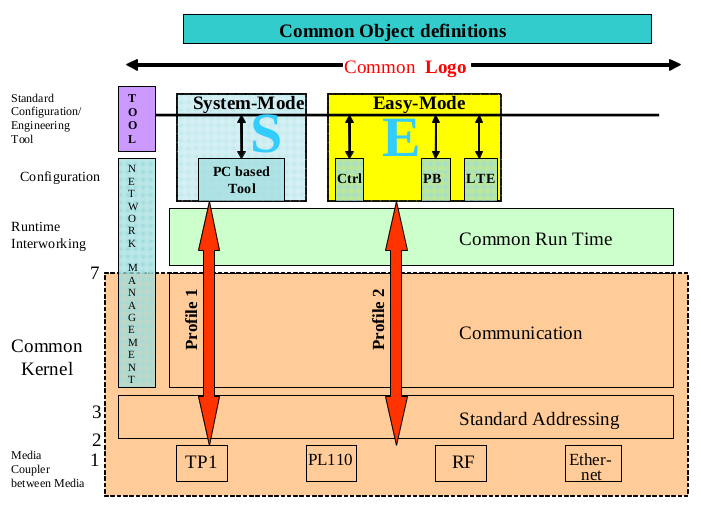
\includegraphics[width=0.8\textwidth]{figures/knx stack.png}
    \caption{The KNX Stack}
    \label{fig:knx_stack}
\end{figure}

\subsection{Datapoints}

Datapoints represent the process- and control variables of the system, and can be of
inputtype, outputtype, diagnostic data, parameters or others. To achieve interoperability,
Datapoints are grouped into functional blocks, implementing standardized datapoint types.

\section{KNX Layers}

The \textit{Open Systems Interconnection Model} OSI standardizes the communication between different, independent systems
by grouping the needed functions into 7 sublayers to provide interchangeability and abstraction. KNX implements this model, omitting 
layers 5 and 6, as shown in figure \ref{fig:knxlayers}. Data from applications are directly passed to the transport layer in a transparent way, and vice versa.

\begin{figure}
    \centering
    \includegraphics[width=0.8\textwidth]{figures/"knx vs iso layers".png}
    \caption{OSI Layer Model, compared to the KNX Model}
    \label{fig:knxlayers}
\end{figure}

\subsection{Physical Layer}

\begin{itemize}
 \item TP1 was inherited from EIB and is the basis medium, consisting of a twisted pair 
 cabeling. Data and power can be transmitted with one pair, so low-power devices can be
 fed over the bus. Data transfer is done asynchronously, with bidirectional, half-duplex
 communication and a datarate of 9600 bit/sec. TP1 uses collision avoidance, and allows
 all topologies beside rings. 
 
 Because this work is base on the TP1 - part of KNX only, this physical layer is explained
in more detail in the next chapter.

 \item PL110, which was also inherited from EIB, uses the power line for communications.
 The carrier uses spread frequency shift keying, also for bidirectional, half duplex 
 communication with a even lower data rate of 1200 bit/sec
 
 \item RF is used for short range wireless communication at 868,3 MHz. 

 \item IP Gateway FIXME
\end{itemize}

\subsubsection{TP1}

The accurate name for this medium is 'Physical Layer type Twisted Pair', with variants
PhL TP1-64 and PhL TP1-256, which is backward compatible to the former one.
\\*
\\*
The logical structure of the TP1 layer is shown in figure\ref{fig:tp1}
\\*
A logical '1' is regarded as the idle state of the bus, so the transmitter
of the MAU(Medium Access Unit) is disabled when sending a '1', so the analog signal on
the bus consists only of the DC part.
\\*A logical '0' is then defined as the voltage drop for a specified duration of t\textsubscript{active},
after which the voltage can increase over DC level, see figure\ref{fig:low}

\begin{figure}
    \centering
    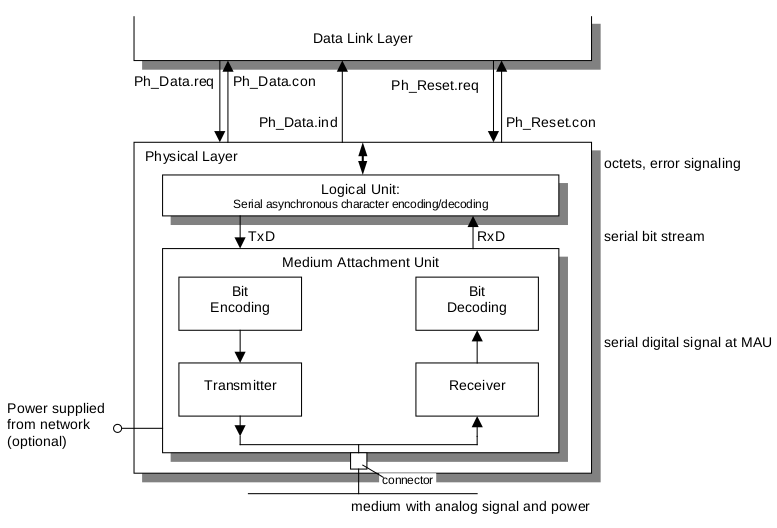
\includegraphics[width=0.5\textwidth]{figures/tp1-structure.png}
    \caption{Logical Structure of TP1}
    \label{fig:tp1}
\end{figure}

\begin{figure}
    \centering
    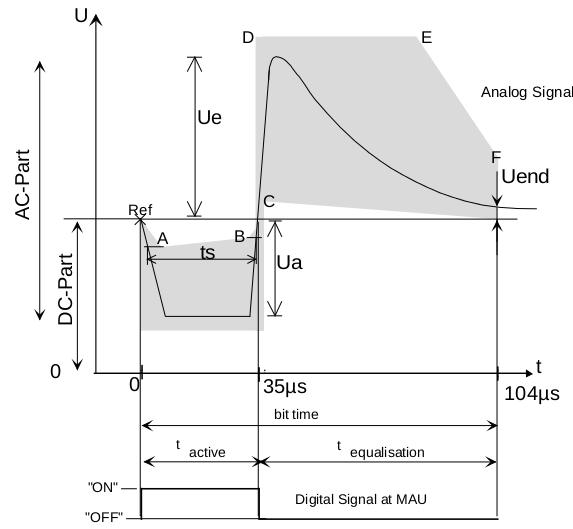
\includegraphics[width=0.5\textwidth]{figures/tp1-low.png}
    \caption{Logical 0}
    \label{fig:low}
\end{figure}

TP1 implements CSMA/CA, so devices will listen to the bus and should only begin sending
when the bus is idle. In the case of a simultaneous transmission start, a logical '1' of one
device will eventually be overwritten by a logical '0' of the other device. The overruled
sender will detect this by continuously checking the state of the bus and has to stop 
transmission.

\subsection{Data Link Layer}

\begin{figure}
    \centering
    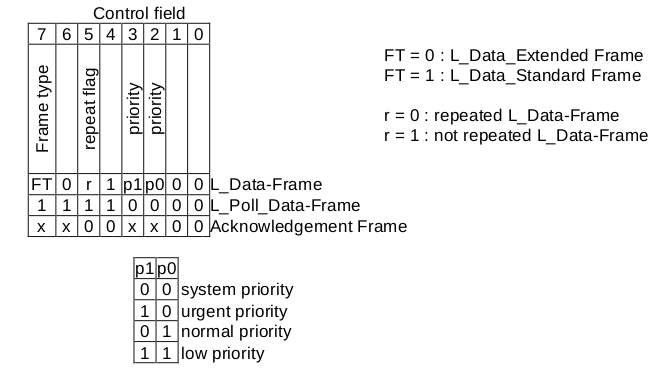
\includegraphics[width=0.5\textwidth]{figures/controlfield.png}
    \caption{Control Field}
    \label{fig:ctrlfield}
\end{figure}

There are defines 3 frame formats which are allowed, each  with the MSB sent first. Every frame starts with a control
field which determines the exact type of the following frame, as shown in figure\ref{fig:ctrlfield}.
In case of the simultaneous start of a transmission, the kind of frame sent, the priority bits of the control field set
or at the latest the source address cause a transmit abortion by the CSMA/CA mechanism used, as explained above.

FIXME
reihenfolge der frames
priority bits are bits 4, 5 --> leading bits <--> priority??


\begin{enumerate}
 \item extended frames
 \item dataframes
 \item repeat frames
\end{enumerate}


\begin{itemize}
 \item L\_Data Frame(Standard or Extended)
 \item L\_Poll\_Data Frame
 \item Acknowledge Frame
\end{itemize}

\subsection{L\_Data\_Frame}

This frame can have two formats: standard\ref{fig:stdframe} and extended\ref{fig:extframe}.
Both start with the control field, for extended frames an extended control field follows.
After that, for booth frames sender address(SA) and destination address(DA), each 2 byte, follow.
The next byte has different meanings: for standard frames, 1 address type bit, 3 
and 4 bits of length information, resulting in an maximum payload of 15 bytes. The extended frame reserves 8 bit of
length information, allowing a maximum payload of 248 FIXME bytes(0xFF is defined as escape code). FIXME

TPCI(transport layer protocol control information) bit - point to point connection.
APCI(application layer protocol control information) bit - read / write / response

For booth formats, a check byte completes the frame, calculating a bitwise NOT XOR function over all bytes.

\begin{figure}
    \centering
    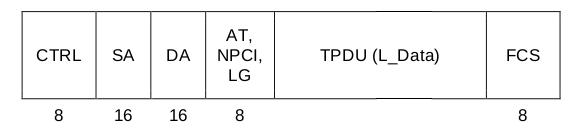
\includegraphics[width=0.5\textwidth]{figures/standardframe.png}
    \caption{Standard Frame}
    \label{fig:stdframe}
\end{figure}

\begin{figure}
    \centering
    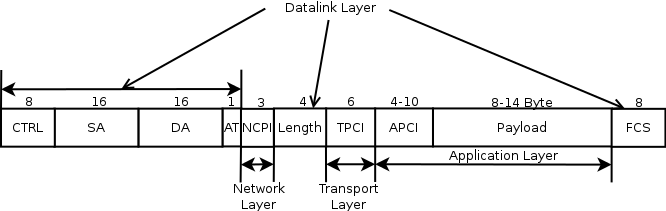
\includegraphics[width=0.5\textwidth]{figures/standardFrame.png}
    \caption{Standard Frame, in detail}
    \label{fig:stdFrameDetail}
\end{figure}

\begin{figure}
    \centering
    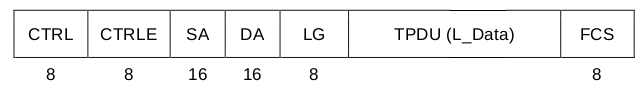
\includegraphics[width=0.5\textwidth]{figures/extendedframe.png}
    \caption{Extended Frame}
    \label{fig:extframe}
\end{figure}

\subsection{L\_Poll\_Data Frame}

These frames serve as data requests for a maximum of 15 bytes(payload of a standard
data frame) and start with a control field, as defined, followed by the 2 byte source address
of the sender(called Poll\_Data Master). The following 2 byte destination address is 
used to address up to 15 poll slaves, all belonging to the same poll group. The number of
exptected bytes and the check octet follow.

Poll requests are answered by poll slaves just by transmitting the databytes without any
special format, sent in the corresponding poll slave slot.

\subsection{Acknowledge Frame}

This frames are used to acknowledge request frames by just sending one byte representing
ACK, BUSY or NOT ACK.

\subsection{Network Layer}

\subsection{Transport Layer}

This layer provides services for reliable point-to-point connections, as well as connection-less point-to-point, 
point-to-domain(multicast) and point-to-all-points(broadcast):

\begin{itemize}
 \item point-to-point, connectionless\\T\_Data\_Individual: connection-less, unreliable point-to-point

 \item point-to-point, connection orientated:
 \\T\_Connect: establish reliable connection to individual address
 \\ 
 T\_Data\_Connected: send data over established connection
 \\ 
 T\_Disconnect: terminate connection to individual address 
 \\
 This service uses a timer to detect timeouts, and allows up to 3 retransmissions. Prior to sending data, a T\_Connect request has to be sent. If the
 remote device cannot handle a new connection, a T\_Disconnect request is returned to the sender. Otherwise, no confirmation or acknowledgment is sent
 to the remote device.
 
 \item point-to-multipoint, connectionless
 \\
 T\_Data\_Group: unreliable multicast to group address

 \item point-to-all-points, connectionless
 \\
 T\_Data\_Broadcast: unreliable broadcast to all devices of a domain

 \item point-to-all-points, connectionless
 \\
 T\_Data\_SystemBroadcast: unreliable broadcast to all devices of a domain FIXME: unterschied Broadcast-SystemBroadcast
\end{itemize}

\begin{figure}
    \centering
    \includegraphics[width=0.8\textwidth]{figures/"transport flags".png}
    \caption{Flags used at the Transport Layer}
    \label{fig:tFlags}
\end{figure}
%FIXME: quellenangabe bild, KNX standard

\subsection{Session Layer}

This layer is left empty in KNX and just forwards data transparently from the lower level to the upper level, and vice versa.

\subsection{Presentation Layer}

This layer is left empty in KNX and just forwards data transparently from the lower level to the upper level, and vice versa.

\subsection{Application Layer}

\subsection{Topologies}

TP1-64 allows up to 64, and TP1-256 up to 256 devices connected to one physical segment in
a linear, star, tree or mixed topology. The maximum distance between 2 devices in one
physical segment is 700m, with all devices in this segment sharing the logical address space
of a subnetwork. 

Up to 4 physical segments are combined by bridges to form lines, guaranteeing a galvanic separation
of these segments and extending the maximum allowed distance between devices, with a maximum
of 255 devices per line. While a bridge itself has no individual address, they acknowledge frames received 
and transmit them on the other side.

Theses lines itself can be combined by routers, forming so called areas, also providing a galvanic separation.


%%%%%%%%%%%%%%%%%%%%%%%%%%%%%%%%%%%%%%%%%

%%%%%%%%%%%%%%%%%%%%%%%%%%%%%%%%%%%%%%%%%
\chapter{EIBD}
\label{ch:eibd}
\section{Setup of the Base System}

The base system consists of a standard raspbian operating system, the EIBD daemon, shared libraries which are used by EIBD and the master daemon.
The operating system is based on the Debian project, with the kernel and all the binaries ported to the ARM platform, so it is possible to use a
comfortable packet manager called
\textit{aptitude} provided by Debian. A short introduction to the most important commands is given below as they are needed.

\subsection{Raspbian}

To obtain a running system for deploying the secure KNX daemon, a prebuilt Debian image is used, which can be ownloaded from the raspberry homepage:

\url{http://downloads.raspberrypi.org/raspbian_latest.torrent}

The image must be unzipped and copied to a suitable memorycard. First-generation raspberries(model 'A') have SD slots, while
all later models come with micro-SD slots. To copy the basic operating system to the memorycard, the linux commandline tool 'dd' can
be used. To find the correct device to write the image to, the following command can be used: 

\begin{lstlisting}[style=BashInputStyle]
    # tail -f /var/log/kern.log
\end{lstlisting}

After inserting the memorycard into a cardreader, look for output like that:

\begin{lstlisting}[style=BashInputStyle]
    [1004111.533698] sdb: detected capacity change from 7909408768 to 0
    [1004114.055840] sd 6:0:0:0: [sdb] 15448064 512-byte logical blocks: ...
\end{lstlisting}

Here, the proper device to use is the device /dev/sdb.
\textbf{Pay attention to use the correct device in the following command - this device will be overwritten}:

\begin{lstlisting}[style=BashInputStyle]
    # dd if=<Path to Image> of=<Device to overwrite>
\end{lstlisting}

After the write command has finished, the memory card is ready to use. For first time setup, a display must be connected via HDMI. Powering up the raspberry
opens a ncurses configuration dialogue. First thing to do is to resize the root partition to maximum size and set a password for the administrative
account. Optionally, different options like keyboard layout can be set.
To be able to operate the raspberry without external display, it is necessary to start the ssh server under \textit{Advanced Options} and assign a 
fixed ip to the host by editing the file \textit{/etc/network/interfaces}, as shown in example \ref{lst:staticIP}. This way it is possible to connect to the raspberry with a ssh client. For password less logins, create an unpriviliged user and
 a ssh public/private key pair for that user by executing these commands on the raspberry pi:

\begin{lstlisting}[style=BashInputStyle]
    # groupadd <usergroup>
    # useradd -g <usergroup> -m <username>
    # su <username>
    # ssh-keygen
\end{lstlisting}
 
The program generates the user and the correspoding key pair and saves public and private key in the subdirectory ~/.ssh/ on the actual host. When asked for a passphrase, it is possible
to use a password-less keypair, an option that should only be used in restriced areas.
To actually use the keypair for logging into
the raspberry pi, the public key must be saved in the file \textit{~/.ssh/authorized\_keys}. Additionally, the private key must be copied to every host
from that ssh connections to the raspberry pi want to be opened. After that, it is possible to load the private key into memory with the command \textit{ssh-add}
and to connect to the host without a password:

\begin{lstlisting}[style=BashInputStyle]
    # ssh-add // only necessary when non-empty passwort is used for keypair
    # ssh <username>@<host-ip|host-dns-name>
\end{lstlisting}

It is also advisable to update the operating system at this time by running the following commands as user root:

\begin{lstlisting}[style=BashInputStyle]
    # apt-get update
    # apt-get install
\end{lstlisting}

This will install the latest package versions of all installed packages. New software can be installed from the command line with these commands:

\begin{lstlisting}[style=BashInputStyle]
    # apt-cache search <pattern> // print a list matching packages for <pattern> 
    # apt-get install <packagename>
\end{lstlisting}

\subsection{EIBD}

The maintainer of EIBD only provides binary packages for the i386 architecture, so the daemon and its prerequisites must be built from source to get
suitable binaries and shared libraries for the ARM environment. Building software under GNU Linux or *nix from source always follows this scheme:

\begin{enumerate}
 \item Downloading and extracting the source code
 \item If possible, comparing the developer supplied hash code  with the hash code of the downloaded source files with
 \textit{sha256} or one of its variants to verify that no modified software has been downloaded.
 \item Optionally, apply patches to the source code(not necessary here).
 \item Set the make-options by calling \textit{./configure <options>}, overriding default compilation options by setting the corresponding command line parameters.
 \textit{./configure --help} should print a list of valid options.
 \item Compiling the source code by calling \textit{make}.
 \item Copying the generated binaries and shared libraries into their correct place by calling \textit{make install}. This last step must always be executed
 as user root because the generated files will be copied into system directories which are not writeable by unprivileged users.
\end{enumerate}

EIBD and the needed library \textit{pthsem} are available from these locations:

\url{https://www.auto.tuwien.ac.at/~mkoegler/pth/pthsem_2.0.8.tar.gz}
\url{http://sourceforge.net/projects/bcusdk/}

After copying the archives to the raspberry, they must be unpacked and compiled. First the pthsem shared library, which offers user mode multi
threading with semaphores, must be compiled because it is used by EIBD. 

\begin{lstlisting}[style=BashInputStyle]
    # tar -xvzf pthsem-2.0.8.tar.gz
    # cd pthsem-2.0.8
    # ./configure
    # make
    # make install // must be executed as root
\end{lstlisting}

This will, among other things, generate the shared library \textit{libpthsem.so.20} in the directory \textit{/usr/local/lib}. \textit{/usr/local}
 is by convention the destination where self compiled software should reside.
Now that pthsem is available, which is a dependence of the EIBD daemon, EIBD itself is ready for compilation:

\begin{lstlisting}[style=BashInputStyle]
    # tar -xvzf bcusdk-0.0.5.tar.gz
    # cd bcdusk-0.0.5
    # ./configure --without-pth-test --enable-onlyeibd --enable-tpuarts
    # make
    # make install // must be executed as root
\end{lstlisting}

first use \gls{svm}
second use \gls{svm}

third use \gls{svm}

\Gls{ssh} is used for login

These steps generate the binary \textit{eibd} and lots of helper programs in the directories \textit{/usr/local/bin}, and the shared object
\textit{/usr/local/lib/libeibclient.so.0} that provides the EIBD API and therefore is needed to be linked to the master daemon. To ease the compilation 
of the master daemon, a makefile has been created. The source of the master daemon is managed by GIT 
%%%%%%%%%%%%%%%%%%%%%%%%%%%%%%%%%%%%%%%%%

%%%%%%%%%%%%%%%%%%%%%%%%%%%%%%%%%%%%%%%%%
\chapter{Mathematical Background}
\label{ch:SOAmath}
 

\begin{itemize}
 \item Divisiblity
 \\
$a | b \iff \exists z \in \mathbb{Z}: b = z \times a$
 \item Integer Division $r \equiv a \bmod b$ 
 \\
 $ \forall a, b \in \mathbb{Z}, b > 0:  a = z \times b + r $ with $ 0 \leq r < b$
 \item Common Divisor $c$ for $a, b \iff$
 \\
 $c | a \wedge c | b$
 \item Greatest Common Divisor(GCD) $d$:
 \\
 $d | a \wedge d | b$ and whenever $c | a \wedge c | b \rightarrow c | d$
 
 \item unlimited number of primes
 \item every number has exact 1 factorization 
\end{itemize}

\section{One Way functions}

The idea for this concept was formulated for the first time in the year 1874 by William Stanley Jevons in his book
'The Principles of Science'(page 144).

%%%%%%%%%%%%%%%%%%%%%%%%%%%%%%%%%%%%%%%%%

%%%%%%%%%%%%%%%%%%%%%%%%%%%%%%%%%%%%%%%%%
\chapter{Cryptopgraphy}
\label{ch:SOAcryptography}
\section{Cryptography}

The tool to achieve information security is cryptography.
Cryptography \footnote{classical greek for \textit{krypt\^{o}s}: \textit{concealed}}
is the science of encrypting information. The evolution of cryptography was no linear process. Ciphers were used independently in different
places, were forgotten and disappeared when the corresponding civilization died. Nevertheless,
basics are found thousands of years ago, therefore a short time table for prominent events is presented:

One of the oldest witnesses for cryptography are hieroglyphs used in Egypt about 2000 B.C., forming the predecessor
of a simple substitution cipher. 500 B.C., the "skytale" was used by greek and spartan military leaders, performing a transposition cipher. Another classical
example was the "Caesar Cipher", used by its inventor about 100 B.C. to hide information by replacing every letter of the alphabet by a letter some fixed number down the alphabet,
thus performing a substitution cipher. Ahmas al-Qalqashandi, an egypt writer, introduced the frequency analysis, a method for breaking substitution ciphers,
in the 14th century. About 300 years later, the "Geheime Kabinets-Kanzlei" in Vienna routinely intercepts, copies and 
 re-seales diplomatic correspondence to embassies, and manages to decrypt a great percentage of the ciphertexts. In the beginning of the 20th century, the 
 first cryptographic device called "Enigma" \footnote{classical greek for "riddle"} is patented for commercial use and is later used in World War 2 by german troops for 
 military communication. Successful attacks against the "Enigma" cipher are demonstrated by polish mathematicians even before outbreak of the war, and systematic
 decryption of "Enigma" - based ciphertexts are conducted in Bleatchley Park, U.K., by using so called "Turing-Bombs", giving the allies invaluable advantages.
The second half of the 20th century brings the introduction of public key cryptography with it: in 1976 Whitfield Diffie and Martin Hellman specify a 
protocol for key exchange, based on a public key system developed by Ralph Merkle, and one year later, the RSA public key encryption is found by the american
mathematicians Rivest, Shamir and Adleman.
\\

Cryptography is basically the art of hiding information by turning cleartext
data into a pseudo-random looking stream or block of bits, called ciphertext, using some kind of
\textit{key}. This process is referred to as \textit{encryption} in general, but it is important to note that for many block ciphers, this encryption process
can also be used to generate a special tag called \gls{mac2}, providing integrity. The next sections deal with how to achieve confidentiality, the 
concepts how to achieve integrity are partially based on the confidentiality methods and are introduced in section \ref{Integrity}
\ref{Integrity}. 
\\
\\
Key, clear- and cipher text all are strings built from the alphabet $\mathcal{A}$. 

\begin{itemize}
 \item $\mathcal{A}$ is a finite set, denoting the alphabet used, for example
 $\mathcal{A} = \{0, 1\}$
 \item $\{0, 1\}^n$ denotes the set of all possible strings with length $n$
 \item $\mathcal{M}$ is the message space, consisting of all strings that can be built with the 
 underlying alphabet
 \item $\mathcal{C}$ is the ciphertext space, also consisting of the strings from 
 the alphbet
$\mathcal{A} = \{0, 1\}$

\item $\mathcal{K}$ is called keyspace, also built from the alphabet. Every element
 $e \in \mathcal{K}$ is called a key and determines the function $\mathcal{M} \rightarrow \mathcal{C}$.
 This function, $E_e$ is called the \textit{encryption function}. 
  \begin{center}
 $ciphertext = E_e(e, cleartext)$
  \end{center}
\end{itemize}

Unauthorized parties - lacking the used key - should, by looking at the ciphertext, learn
absolutely nothing about the hidden cleartext beside the length of the origin message. Authorized parties, on the other hand, are
able to retrieve the original data out of the ciphertext by using the key with polynomial work, thus reversing
the encryption. This reversing process is called \textit{decryption}.

\begin{itemize}

 \item For every key $d \in \mathcal{K}$, $D_d$ denotes the function from $\mathcal{C} \rightarrow
  \mathcal{M}$, and is called \textit{decryption function}.
  \begin{center}
  $cleartext  = D_d(d, ciphertext)$
    \end{center}
\end{itemize}

The keys $e$ and $d$ are also referred to as \textit{keypair}, written $(e,d)$. 
If it is computationally easy to derive the private key $e$ from the public key $d$ (in most cases $e = d$), the encryption scheme
 is called \textit{symmetric}, otherwise the scheme is called \textit{asymmetric}.

Combining this properties yields a cipher or \textit{encryption scheme} defined over $\mathcal{(K,M,C)}$, which is a pair of \textit{efficient}
 \footnote{"runs in polynomial time"} algorithms s.t.
 \begin{center}
   $\mathcal{K} \times \mathcal{M} \rightarrow \mathcal{C}$
   \\
   $\mathcal{K} \times \mathcal{C} \rightarrow \mathcal{M}$
 \end{center}

 The correctness property ensures for every pair of $(e,d) \in \mathcal{K}$ and for every message $m \in \mathcal{M}$ that encryption is reverseable, i.e. 
 it must hold that 
 \begin{center}  
 $ m = D_d(d, (E_e(e, m))$
  \end{center}

\subsection{Kerckhoff's Principle}

When designing cryptographic systems, a fundamental question is what components of it must be protected from public knowledge, and what parts can be published without
compromising the security of the system. A cipher is considered secure if it is not breakable by an adversary in a reasonable time frame \cite{handbook1}, where
this time frame is a function of the useful timespan of the protected data. This synonymously means that an adversary must spend exponential work.
It follows that \textit{every} cipher can be broken in principle by
mounting the "brute-focrce" attack, searching the correct $n$-bit key in the exponential big key space $2^n$. Thus, such an exhaustive search must be rendered impracticable by 
using a suitable large key space to obtain a secure cipher.

The dutch cryptographer Auguste Kerckhoff added some additional rules for designing a secure cipher.
According to \textit{Kerckhoff's Principle} stated 1883, among other properties, a secure system should not rely on the secrecy of
its components, the only part that should be kept secret is the key alone.  

Mapped to the definitions above, the sets $\mathcal{M, C, K}$, as well as the
transformation functions $E_e$ and $D_d$, must not secret. The only thing that has to be kept private is the decryption key $d$.

This separation of key and algorithm allows the publication of the basic cipher methods, benefiting from peer review. The contradicting approach by trying
to hide the inner workings from public to increase security is also known as "Security by Obscurity".
\\

Another definition of a secure cipher was introduced by Shannon in 1949 \cite{6769090}, viewed from a communication-theory point of view. Depending on the
message space, there is a finite number of possible cleartext messages, each occurring with its own \textit{a priori} probability. These messages are encrypted
and sent to the receiver. An eavesdropper, intercepting messages, can calculate the \textit{a posteriori} probabilities for all possible cleartext messages, 
leading to the observed cipher text. If booth probabilities are the same, the attacker has learned absolutely nothing from intercepting the cipher text, which
is defined by Shannon as \textit{perfect secrecy}. A prerequisite for a perfectly secure cipher is that the key space is at least as big as the message space.
Otherwise there will exist cleartext messages which are mapped to the same cipher texts, and thus a priori and a posteriori probabilities will be different,
allowing the attacker to get knowledge he should not have gotten.
\\

In contrast, \textit{semantic} security can be seen as a weaker form of security, namely perfect secrecy against an adversary having only polynomially bounded
processing powers.
\\

Because all cryptographic schemes rely on the generation of random numbers, a short introduction to probabilistic theory and \gls{prng} is given,
followed by a introduction to the most important representatives for symmetric and asymmetric ciphers.

\section{Randomness and Probabilistic Theory}

A basic requirement of all cryptographic schemes is the availability of randomness. \textit{Entropy}, denoted $H$, is the unit of the unpredictability of a process, as
 defined by Shannon in \cite{6773024}:
 
\begin{align}
 H(X) = - \sum_{x \in X}^{} p(x) * ln(p(x))
\end{align}


The higher the predictability, or in other words, the more likely an event, the lower its entropy. Flipping a "fair" coin is a canonical 
example of a process with maximum entropy, because every coin flip has a probability of $\frac{1}{2}$, and all flips are independent from each other \cite{1621063}.
If obtaining heads of the coin is viewed as a logical "0" and tails as a logical "1", a binary string of length $n$ can be built, where the probability of all possible
strings of same length is equal, as shown in figure \ref{fig:uniform}, yielding an \textit{uniform distribution}, with
$H = 2^n*\frac{1}{2^n}*ln(2^n) = n$ bit. 
\\
\\
The importance of random numbers in cryptography is founded on the nature of the cipher used, as will be shown in the next sections. For example,
stream ciphers generate a keystream which is used
for encryption. If the keystream is predictable by an adversary, the security of the cipher is reduced. Similar arguments are valid for block ciphers, which often
rely on an initial value called \gls{iv} for encryption. Also, many key negotiation algorithms schemes rely on determining a random prime number, which is often 
achieved by choosing a random number and testing it for primality. Again, if such a prime number can be narrowed down within some boarders, this fact may
weaken the encryption process.

A fundamental problem in generating random numbers by utilizing computing devices is the deterministic nature of an algorithm:
\\

\textit{"Anyone who considers arithmetical methods of producing random digits is, of course, in a state of sin."} \footnote{John von Neumann, 1951}
\\

Such numbers are therefore called \textit{pseudo}random. Lots of cryptographic products suffered serious flaws because of relying on a broken \gls{prng}. A 
historical example of such a broken random number generator, outputting biased (i.e., not uniformly distributed values) was "RANDU", invented by IBM in the
1960s. 
The generator belongs to the class of multiplicative congruential algorithms as proposed by Lehmer \cite{MR0044899}, which can in principle generate random
numbers of sufficient quality, \textit{if} the correct parameters are chosen.
Random values can be obtained after setting an initial value for $I_0$, called \textit{seed}, and repeatedly executing the calculation

\begin{center}
 $I_{j+1} = 65539 * I_j \pmod{2^{31}}$
\end{center}

One problem 
is that consecutive values generated by RANDU are not independent, a fact that	 can be seen in figure \ref{fig:randu}. To obtain the plot, 10000 uniformly distributed 
random numbers were chosen as initial seeds for $I_i$ and plotted as x-values. $I_{i+1}$ served as y- and $I_{i+2}$ as z-values. While one would suspect that all points
would be equally distributed in space, a clear pattern is visible, indicating that the values are correlated.

To assess the quality of a \gls{prng}, beside of such spectral tests lots of additional tests are available, see \cite{nistRAND} for details.

To encounter the shortcomings of a \gls{prng}, a \gls{trng} uses a natural process as non-deterministic data source, for example
thermal noise of a semi conductor, cosmic noise from space or digital oscillators.

The used hardware platform, the RapsberryPi, offers a hardware number generator - the quality of its provided random numbers will be subject
to various statistical tests, see chapter \ref{FIXME} for the results.

\begin{figure}
    \centering
    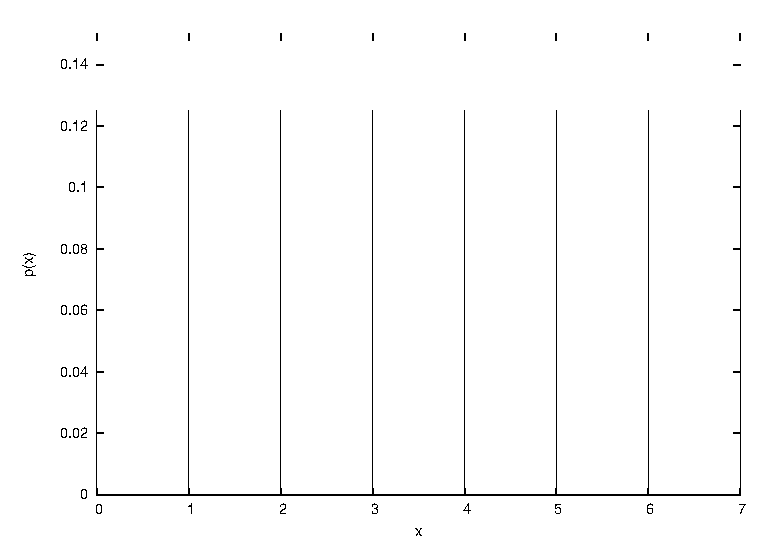
\includegraphics[width=0.6\textwidth]{figures/uniform}
    \caption{Uniform Distribution of binary string of length 3}
    \label{fig:uniform}
\end{figure}

\begin{figure}
    \centering
    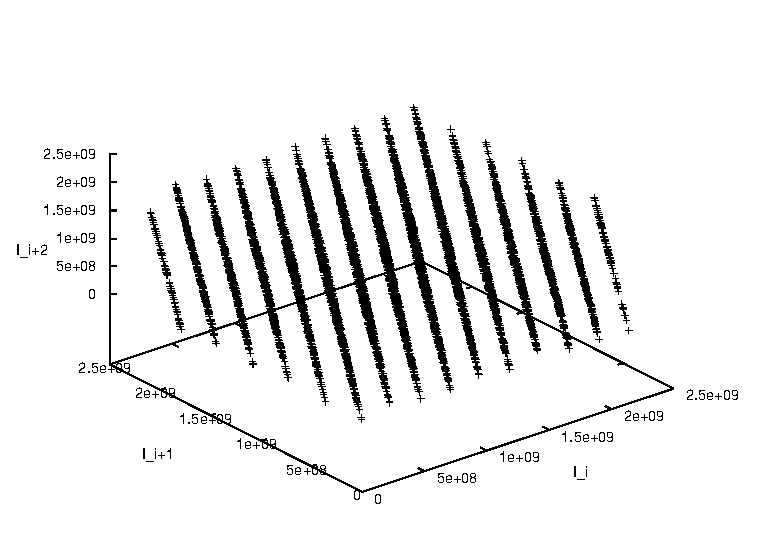
\includegraphics[width=1\textwidth]{figures/randu}
    \caption{Spectral Plot of RANDU output}
    \label{fig:randu}
\end{figure}


\section{Symmetric vs. Asymmetric Cryptography}

As stated above, two very fundamental differences regarding the key used in a cryptographic system can be found. Symmetric ciphers, where 
the same key is used for encryption and decryption, outperform its asymmetric counterparts in regards of data throughput by a factor of about 1000 \cite{5412055}.
Additionally, they need shorter keys to achieve the same level of security - both arguments encourage it's use in embedded devices because of its less computing
and memory demands.

The big disadvantage of symmetric ciphers is that the key must be known to sender
and receiver of the message \textit{before} secure communication can take place. This constitutes some kind of chicken-egg problem: to be able to send encrypted
data, the key must be distributed, i.e. a secure channel has to be setup first for key exchange. But if such a secure channel can be established, it could also be used
for transmitting the sensitive data themself.
\\

Asymmetric or public key cryptography solves the problem of key distribution by using two different keys, belonging to the same key pair: the \textit{private}
key must be be protected from disclosure, while the \textit{public} key can be published without harming security. For encryption, the public key of the receiver
is used, who in turn will use his private key to decrypt the message. 

To be able to take benefit from the advantages of booth schemes, a hybrid approach is possible: at first, public key cryptography is used to negotiate a symmetric session
key, which then can be used to encrypt the actual, sensitive data.

\subsection{Stream Ciphers}

Most stream ciphers belong to the family of symmetric ciphers, thus $e_i = d_i$. The reason is that most asymmetric ciphers are deterministic ciphers,
i.e. the encryption of the same message with a fixed public key always yields the same cipher text. Thus, such repeated messages can be detected by 
an adversary. 
Probabilistic public-key encryption can solves this problem for stream ciphers,
but this scheme will not be handled in this work because of its low practical application.

For encryption, stream ciphers take arbitrary long messages (from the message space $\mathcal{M}$), and encrypt
them to the corresponding ciphertext(out of the ciphertext-space $\mathcal{C}$), by applying
one digit of the message to one digit of the key. It is valid to say that a streamcipher is a block cipher with blocklength 1.

\begin{itemize}
 \item A keystream is a sequence of symbols $e_0, e_1, ..., e_n$, all taken from the keyspace $\mathcal{K}$
\end{itemize}

The encryption function $E_e$ performs the substitution $c_i = E_e(e_i, m_i)$, producing one encrypted symbol at a time. Analogously,
the decryption function inverts this substitution: $m_i = D_d(d_i, c_i)$.

\subsubsection{The Vernam Cipher} 

This cipher, also called \gls{otp}, was invented by Gilbert Vernam in 1918, and belongs to the family of polyalphabetic stream ciphers,
which means that every character of the origin message is mapped to another character of the same alphabet. In contrast to a monoalphabetical cipher,
there is no fixed mapping between the input and output characters.
The substitution is achieved by generating a keystream and by executing 
a bit-wise \gls{xor} operation, as defined in table \ref{table:xor}, of key and message.

\begin{center}
\begin{tabular}{ c c | c }
 \label{table:xor}
   &  & $\bigoplus$ \\ \hline
  0 & 0 & 0 \\
  0 & 1 & 1 \\
  1 & 0 & 1 \\
  1 & 1 & 0 \\
\end{tabular}
\end{center}

Decryption can be achieved by applying the \gls{xor} operation to key and ciphertext:

\begin{center}
 $m_i = c_i \bigoplus k_i = (m_i \bigoplus k_i) \bigoplus k_i = m_i$, with $ k_i \bigoplus k_i = 0, const \bigoplus 0 = const$
\end{center}


Obviously, the security of the cipher heavily depends on the quality of the \gls{prng}. If a truly random source is used to generate the key stream, this cipher
has perfect secrecy: for a n-character ciphertext, \textbf{all} n-character cleartexts are equally probable, and vice versa. 
The reason for this is the \gls{xor} operation: booth possible outcomes are booth equally probable, introducing one bit of randomness into every data bit. 

Additionally, the \gls{xor} operation can be built easily in hardware, accelerating the encryption or decryption process.

Nevertheless, the cipher can be completely broken if the same key is used for encrypting more than one cleartext message, allowing to mount
an attack based on frequency analysis.
If an attacker is able to intercept a high number of different ciphertexts, all encrypted with the same key, the pairwise xor'ing of the ciphertexts
yields the xor-combination of the corresponding cleartexts, because
\begin{center}
 $m_1 \bigoplus m_2 = (c_1 \bigoplus k) \bigoplus (c_2 \bigoplus k) = c_1 \bigoplus c_2 \bigoplus k \bigoplus k = c_1 \bigoplus c_2 \bigoplus 0 = c_1 \bigoplus c_2$
\end{center}

Whenever the same character is present in two different ciphertexts at the same position, the result of the \gls{xor} operation will be 0x00, allowing to draw
inferences about the language used. By utilizing frequency analysis, the used key can be determined position by position with effort bounded by $O(n^2)$.

\subsubsection{Stream Ciphers based on \gls{lfsr}}

An disadvantage of the Vernam cipher is that a key of equal length as the message is necessary. To mitigate this problem, a \gls{lfsr} can be used to generate
a key of proper length from a much shorter, initial key. Such \gls{lfsr} are denoted by $\langle L, C(D) \rangle$. $L$ is the number of stages, and $C(D)$ is the
\textit{connection polynomial}. Because of the finite length, every \gls{lfsr} can only take on a finite number of internal states, producing
a periodic output sequence.
If the degree of the connection polynomial is equal to the number of stages and the connection polynomial is irreducible (i.e. the polynomial can not
be factored into 2 non-constant polynomials), no matter of the initial state, the output sequence produced will always be of maximum periodicity.

Figure \ref{fig:lsfr} shows a 4 stage non-singular \gls{lfsr} with

\begin{center}
 $L=4$,  $C(D) = 1 + D + D^4$,
\end{center}

Table \ref{table:lfsr} \cite{handbookLFSR} shows the corresponding output sequence produced. After
15 shifts a state equal to the initial state is achieved, and the outputs
begin to repeat.

While such \gls{lfsr} can be easily built in hardware, a problematic fact remains that their \textit{linear complexity} is bounded by $L$. Therefore, a \gls{lfsr}
should never be used as keystream generator directly, instead the outputs of different \gls{lfsr} are combined by a non-linear function, thus obtaining a
nonlinear generator.

\begin{figure}
    \centering
    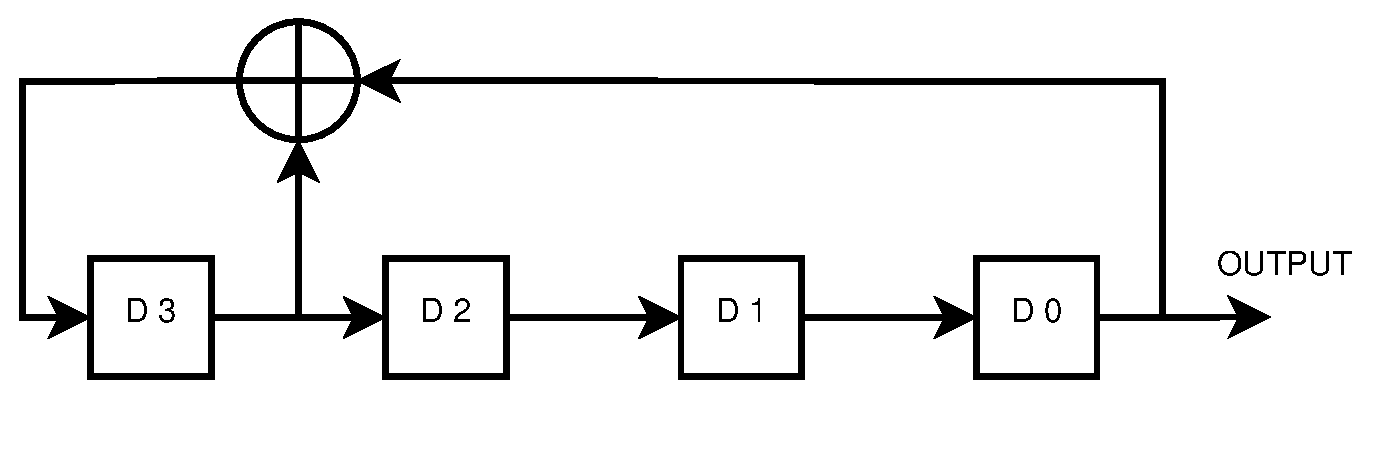
\includegraphics[width=1\textwidth]{figures/LSFR}
    \caption{4 Stage LFSR}
    \label{fig:lsfr}
\end{figure}

\begin{center}
\begin{minipage}{0.45\textwidth}
\begin{tabular}{ c | c | c | c | c }
 \label{table:lfsr}
  t & $D_3$ & $D_2$ & $D_1$ & $D_0$ \\ \hline
  0 & 0 & 1 & 1 & 0 \\
  1 & 0& 0& 1& 1\\
  2 & 1&0 &0 &1 \\
  3 & 0& 1& 0& 0\\
  4 & 0&0 &1 &0 \\
  5 & 0&0 &0 &1 \\
  6 & 1&0 &0 &0 \\
  7 & 1&1 &0 &0 \\
  \end{tabular}
\end{minipage}\hfill
\begin{minipage}{0.45\textwidth} 
\begin{tabular}{ c | c | c | c | c }
  t & $D_3$ & $D_2$ & $D_1$ & $D_0$ \\ \hline
  8  & 1& 1& 1& 0\\
  9  & 1& 1& 1& 1\\
  10 & 0& 1& 1& 1\\
  11 & 1& 0& 1& 1\\
  12 & 0& 1& 0& 1\\
  13 & 1& 0& 1& 0\\
  14 & 1& 1& 0& 1\\
  15 & 0& 1& 1& 0\\
\end{tabular}
\end{minipage}
\end{center}

\subsection{Block Ciphers}

These ciphers operate on input blocks of fixed size, transforming them into output blocks of same size. This implies that larger messages must be broken into
suitable blocks, and that for the last remaining block it may be necessary to add padding bytes to yield the full block size,
adding overhead to the message - a disadvantage compared to stream ciphers. For example, to encrypt a message just exceeding the block size by one byte,
for the excess byte a complete block must be concatenated. 

On the other hand, while stream ciphers are strictly sequential by nature, there exist methods to speed up block ciphers by splitting the message
first, and then process them in parallel\footnote{Counter Mode, see \ref{confidentiality}}. 
\\
Two main types of block cipher exist: \textit{transposition} ciphers use a key-dependent permutation to re-order the characters of the block to obtain the ciphertext.
This is a bijective transformation, so decryption can be achieved by simply reversing the permutation.

Substitution ciphers define a key-dependent mapping of characters from the alphabet $\mathcal{A}$ to the same alphabet, thus replacing every character by one
or more other characters. In the latter case, this equals an injective function which can not be reversed directly.
 
A product cipher is a combination of ciphers of different types to achieve a higher level of security than possible as with the basic ciphers. 
\\

Feistel networks are special product ciphers, composed of \gls{sp} networks. They were first described by Horst Feistel in the year 1973\cite{feistel}, and are 
the basis of a variety of block ciphers like "LUCIFER" \cite{feistel1974block,}, developed by Feistel, and \gls{des}.

Figure \ref{fig:feistel} shows the principal layout of such ciphers: at first, the plaintext block of length
2n-bits is divided into two n-bits blocks, often called $L_0$ and $R_0$ for left and right block, respectively. After that the first round starts: every round
is characterized by performing a substitution, followed by a permutation of the two half-blocks. For substitution, at first a \textit{round function},
parametrized by a \textit{round key} is applied to one half of the data block, followed by a \gls{xor} operation. The output of the rounds can be calculated
according to the formulas shown in \ref{table:feistel}
\\

\begin{center}
\begin{tabular}{ l l}
 \label{table:feistel}
  Encryption of round 1: & $L_1 = R_0$  \\ 
   &  $R_1 = L_0 \bigoplus F(k_1, R_0)$\\ \hline
  Encryption of round 2: & $L_{2} = R_1$  \\
   &  $R_{2} = L_1 \bigoplus F(k_2, R_1)$ \\ \hline
   ... &  \\ \hline
   Encryption of round n: & $L_{n} = R_{n-1}$ \\
   & $R_n = L_{n-1} \bigoplus F(k_n, R_{n-1})$ \\
\end{tabular}
\end{center}

Decryption is achieved by applying the ciphertext to the same network, with the round keys applied in reverse order, reducing hardware- respectively
code size, as shown in \ref{table:feistelRev}. Because decryption does not rely on reversing the round function, there is no necessity for the round function to be bijective.
\\

\begin{center}
\begin{tabular}{ l l}
 \label{table:feistelRev}
Decryption of round n: & $R_{n-1} = L_n$  \\
 & $L_{n-1} = R_n \bigoplus F(k_n, R_{n_1}) = R_n \bigoplus F(k_n, L_{n}) $
\end{tabular}
\end{center}

\begin{figure}
    \centering
    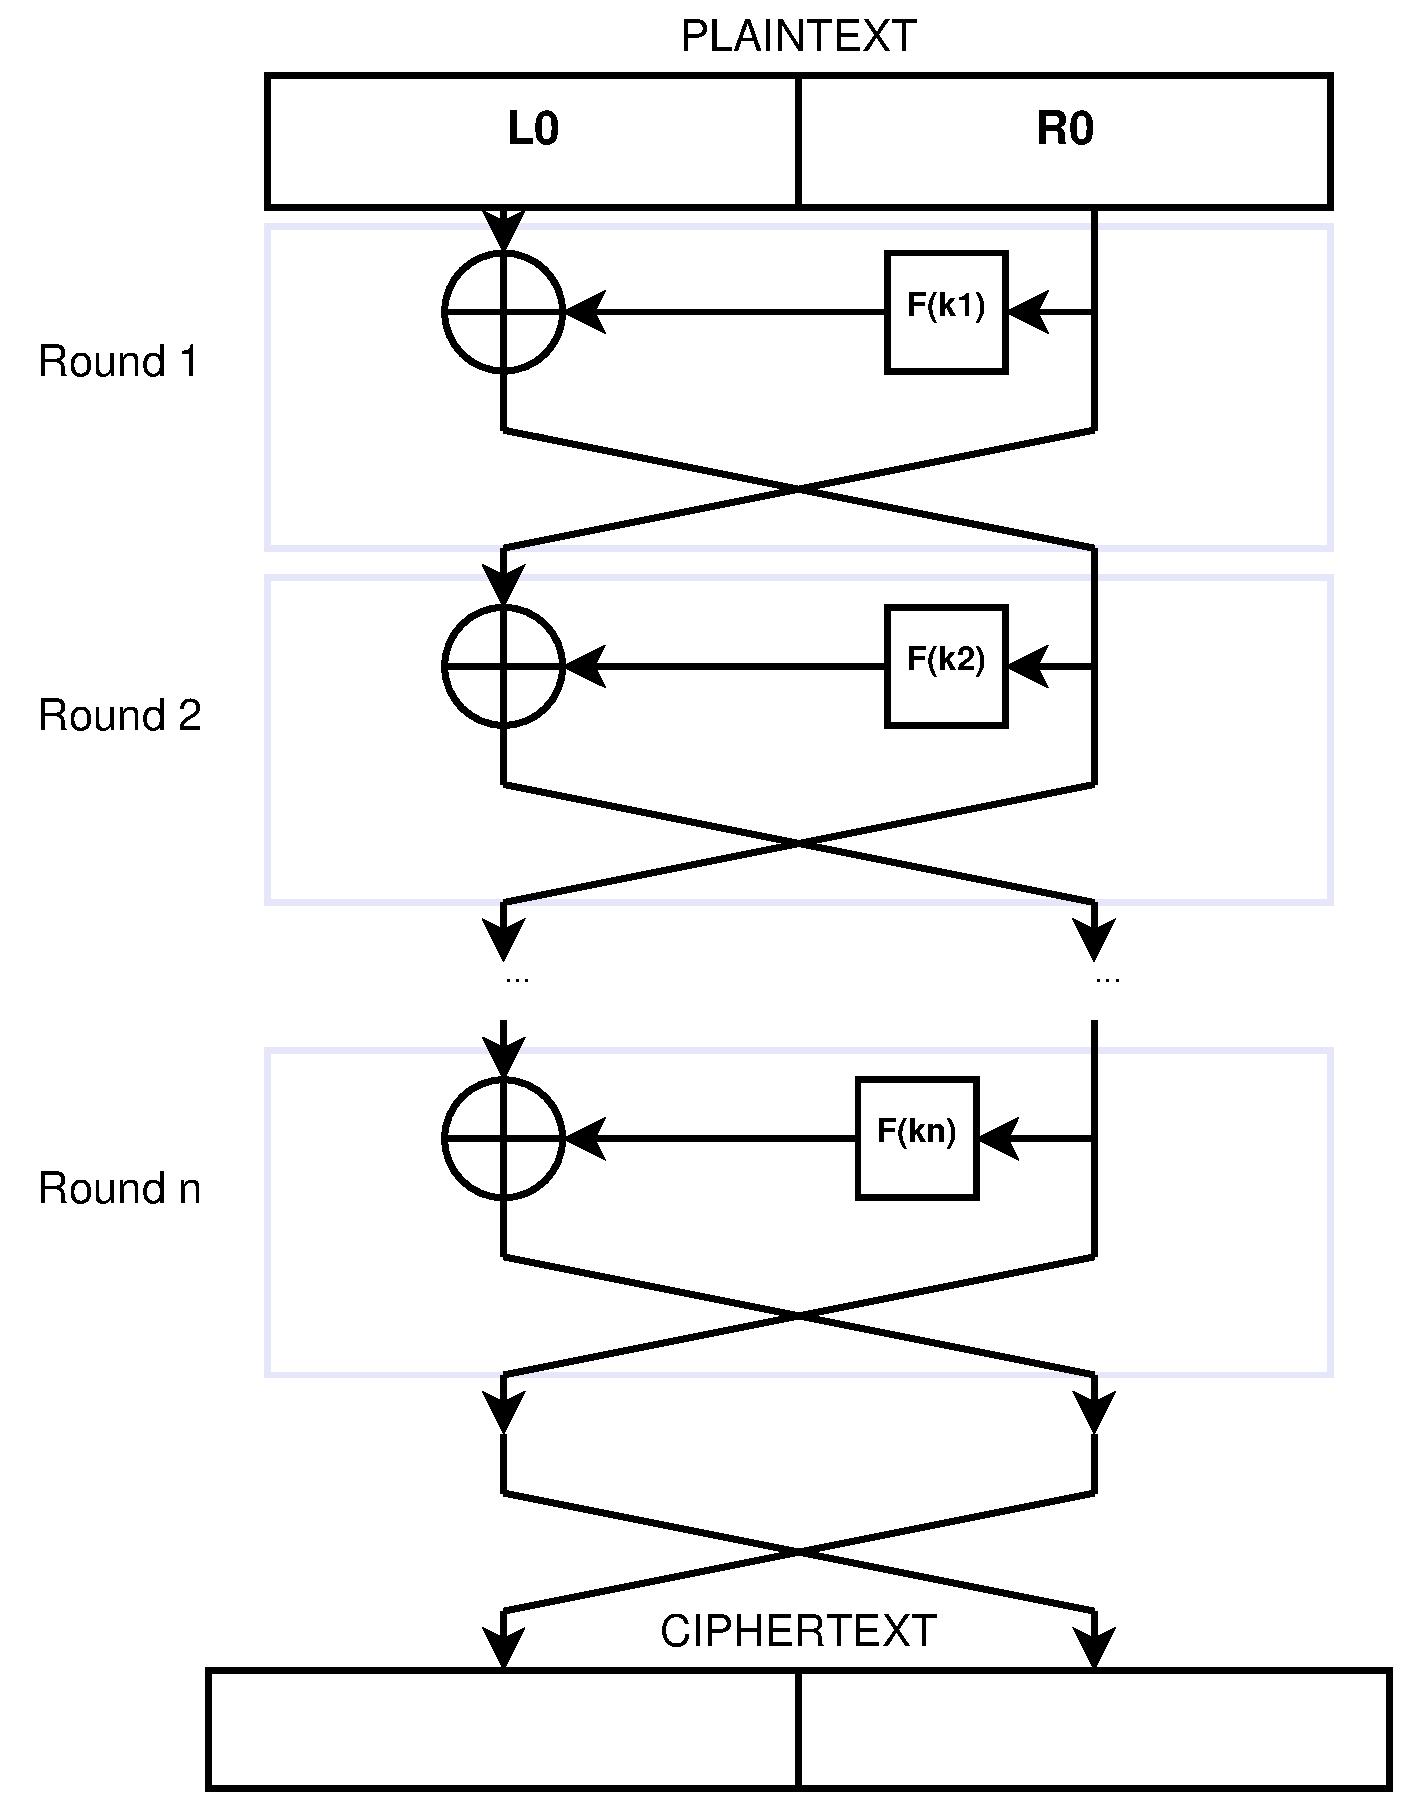
\includegraphics[width=0.5\textwidth]{figures/feistel.eps}
    \caption{Feistel Substitution-Permutation Network}
    \label{fig:feistel}
\end{figure}

\subsubsection{\gls{des} and \gls{3des}}

\gls{des}, designed by IBM and published by \gls{nist} in 1977 \cite{des}, encrypts 64 bit blocks in 16 processing rounds.

For every round, a 56 bit round key is derived from the basic 56 bit
key by permutations. The 64 bit data block to be encrypted respectively decrypted is subjected to an initial permutation and then feed into the Feistel
network. The round function operates as follows:

At first, the 32 bit half block is expanded to 48 bit by copying specific bits. The outcome is added to the round key modulo 2 (i.e., the \gls{xor} operation).
Next, a non-linear transformation is applied by so-called "S-Boxes", performing a surjective function by substituting blocks of 6 bit by only
4 bit. Lastly, a deterministic permutation follows, achieved through "P-Boxes", concluding the round
function.

Because of the small key size, \gls{des} was successfully broken for the first time\footnote{At least officially - rumors about the involvement of the \gls{nsa}
regarding the small key size and the design of the S-Boxes existed since the publication} by a brute-force attack in 1997.

To prevent such attacks, \gls{3des} was published: the cleartext- respectively 
cipertext block is feed 3 times to the \gls{des} cipher, using 3 different keys $k_1, k_2, k_3$ to first encrypt with $k_1$, decrypt with $k_2$ and finally 
encrypt with $k_3$, effectively tripling the key size:

\begin{center}
 $ciphertext = E(k_3(D(k_2,E(k_1, cleartext)))$
\end{center}

The special sequence of encryption, decryption and again encrypting was chosen because by setting $k_1 = k_2 = k_3$, a \gls{3des} implementation can also be used
for en/decryption of \gls{des} messages.

\subsubsection{\gls{aes}}

Also called "Rijndael" after its developers Joan Daemen und Vincent Rijmen, \gls{aes} is is the successor of \gls{3des}, as
proposed by the \gls{nist} in 2001. Basic properties are a block size of 128 bit, and possible key sizes
of 128, 192 or 256 bit.

The operation, shown in figure \ref{fig:aesEnc}, starts by copying the input block into a square matrix, called "State",
followed by a \gls{xor} combination of the first round 
key and the matrix. Then, 9, 11 or 13 rounds, depending on the key size, are performed: substitution by S-Boxes, permutation by shifting rows, 
another substitution by mixing columns and applying the round key. A last round, omitting the mix-columns stage, concludes the encryption.
Operating on the whole data block, \gls{aes} is not a Feistel network, therefore all substitutions and permutations must be reversible to allow decryption: 
the S-Box used here is therefore implementing byte-by-byte substitutions. The round keys are derived from the origin key by the \gls{aes} key expansion.

\begin{figure}
    \centering
    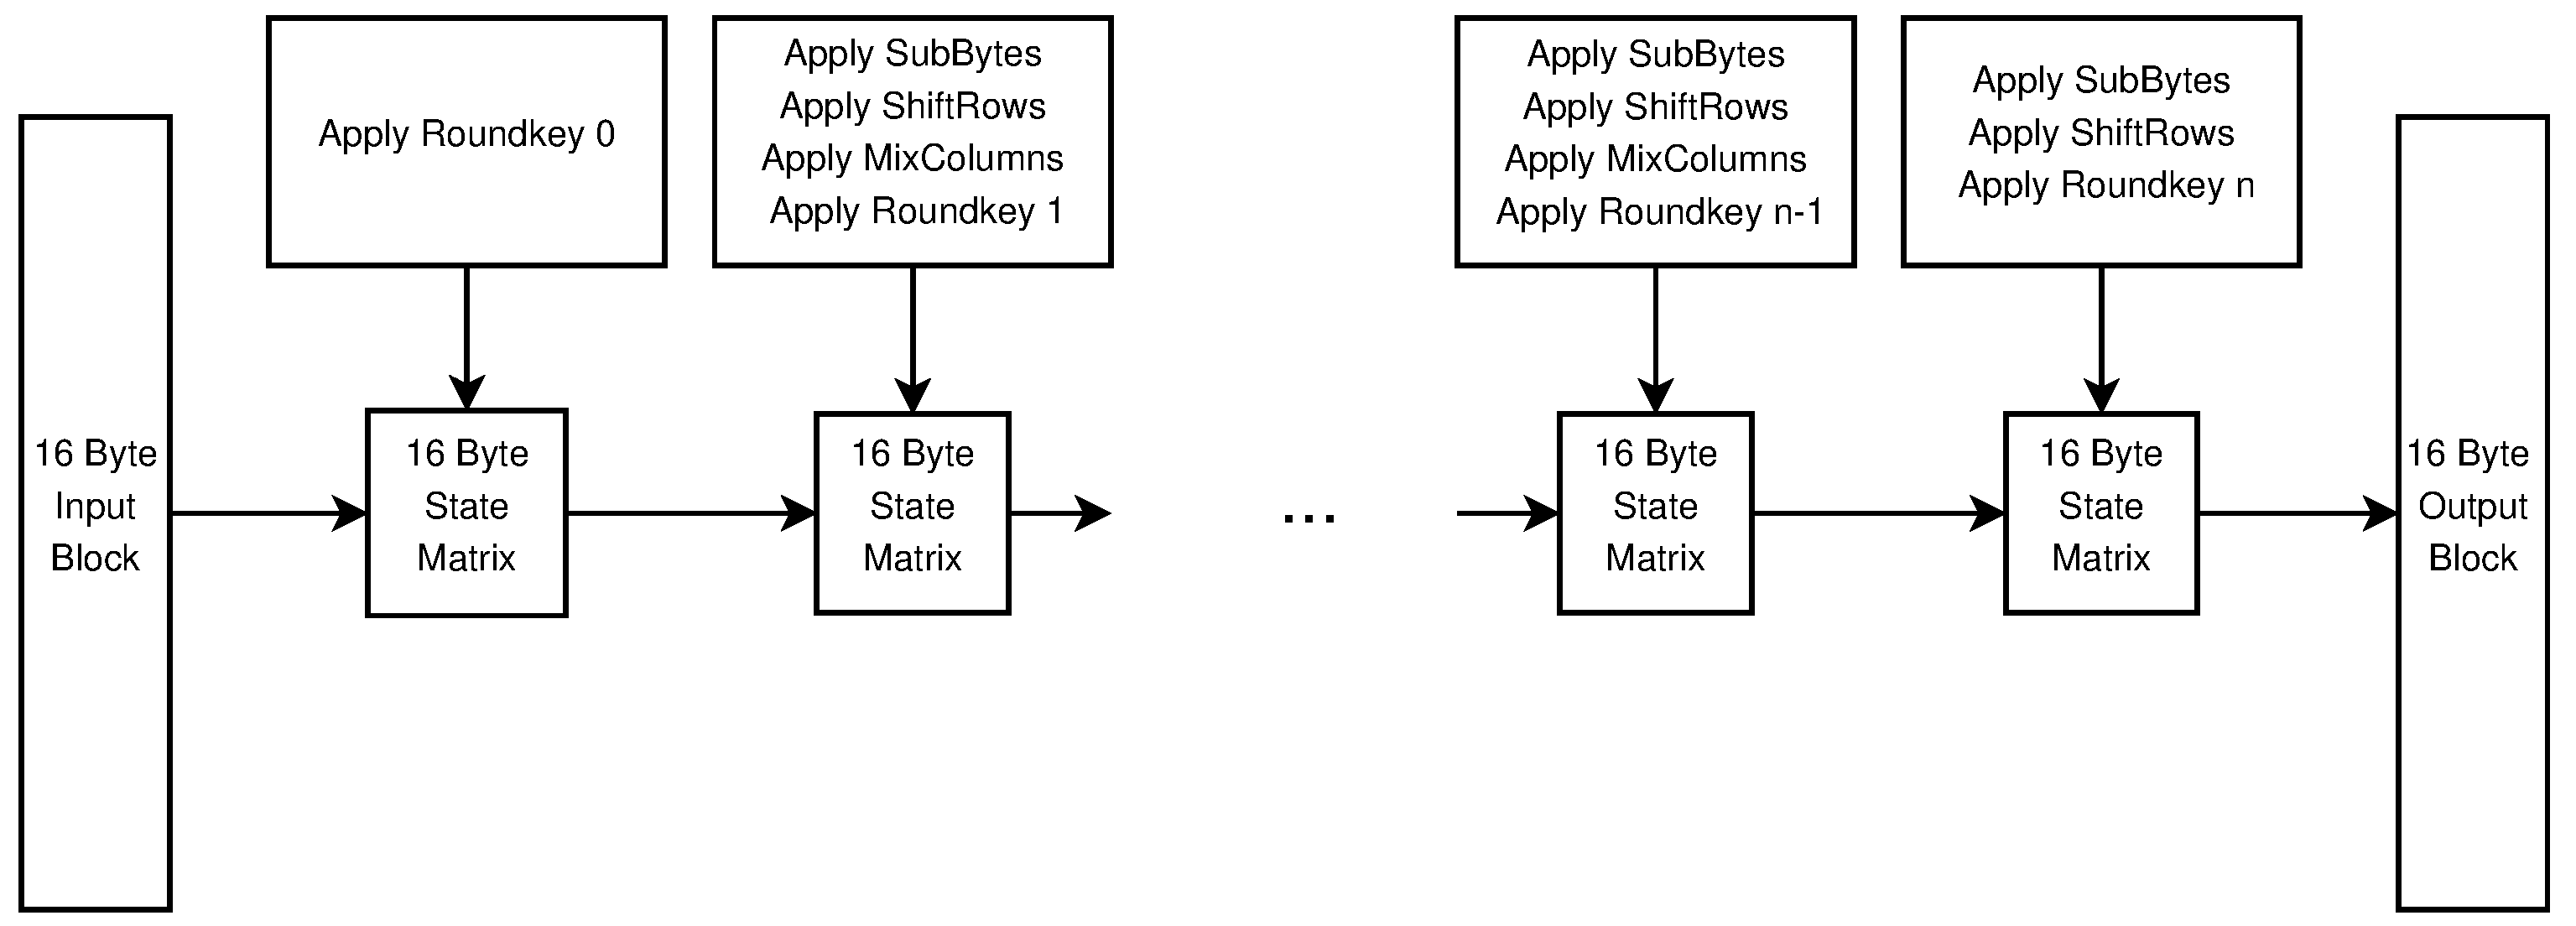
\includegraphics[width=1\textwidth]{figures/aesEnc.eps}
    \caption{AES Encryption Process}
    \label{fig:aesEnc}
\end{figure}

Decryption uses the round keys in reverse order. To reverse the first substitution of every round, a unique inverse S-Box is used, while the shifting rows
and mixing columns can also be reversed.
\\

FIXME: S-Box berechnung erklaeren?? stallings, principles and practice 

\subsection{Mode of Operation}\label{confidentiality}

Because block ciphers  operate on a fixed number of bytes, messages larger than this block size must be broken into parts of suitable size, and depending on 
the resulting size of the last block, it may be necessary to append a padding to it. Five different such modes were defined by \gls{nist} in 2001 \cite{moo},
which will be introduced in the next sections. For all modes it does not matter what underlying block cipher is used, as long as the block cipher implements
a cryptographic secure function. 

An important property of this modes is the error propagation.
Whenever a bit error occurs on the transmission channel due to noise or interference,
a logical '0' of the transmitted cipher text is substituted by a logical '1' or vice versa. This bit error in the cipher text produces one or more bit errors
in the clear text, thus the name error propagation \cite{burda}.

\subsubsection{\gls{ecb}}

\gls{ecb} can be used to gain confidentiality and allows the parallel processing of all input blocks. This mode does not use any \gls{iv} or nonce, therefore
repeating input blocks are mapped to the same output blocks under the same key. This is problematic, which can be seen quite intuitively by comparing 
figures \ref{fig:tuxclr} and \ref{fig:tuxecb}. Therefor this mode should be avoided.

 \begin{minipage}{\linewidth}
      \centering
      \begin{minipage}{0.4\linewidth}
          \begin{figure}[H]
              
\includegraphics[width=\linewidth]{figures/TuxCleartext.png}
              \caption{Unencrypted Picture}
              \label{fig:tuxclr}
          \end{figure}
      \end{minipage}
      \hspace{0.05\linewidth}
      \begin{minipage}{0.4\linewidth}
          \begin{figure}[H]
              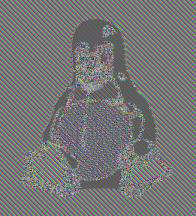
\includegraphics[width=\linewidth]{figures/TuxECB.png}
              \caption{\gls{ecb} encryption of the picture}
              \label{fig:tuxecb}
          \end{figure}
      \end{minipage}
  \end{minipage}

\subsubsection{\gls{cbc}}

This mode uses an \gls{iv} and can therefor be used for encryption of same messages without changing the key. Additionally, \gls{cbc} can also be used
for \gls{mac2} generation, as explained in section \ref{cbcAuth}.

Encrypting a message is shown in figure \ref{fig:cbc_encrypt}.

\begin{center}
$ C_0 = E(k, (M_0 \bigoplus IV ) )  $
\\
$ C_1 = E(k, (M_1  \bigoplus C_0) ) $
\\
$...$
\\
$ C_i = E(k, (M_i \bigoplus C_{i-1} ) )  $
\end{center}

To reverse the process, i.e. decrypt the message, see figure \ref{fig:cbc_encrypt}

\begin{center}
$ M_0 = D(k, C_0) \bigoplus IV $
\\
$ M_1 = D(k, C_1) \bigoplus C_0 $
\\
$...$
\\
$ M_i = D(k, C_i) \bigoplus C_{i-1} $
\end{center}

The \gls{iv} does not have to be kept private, but must be known to the receiver of the message. It is important that such an \gls{iv} is unpredictable, otherwise
allowing a \gls{cpa}. Also, it must not repeat over the lifetime of the key, otherwise introducing the \gls{ecb} problem again. 

The \gls{iv} introduces overhead, which is more problematic for  shorter messages.
To avoid such a message expansion, a solution is to use a "nonce", which stands for "\textit{n}umber used \textit{once}", as suggested in \cite{cryptoEng}.
Sender and receiver must maintain a message counter. This message counter must be encrypted to avoid predictability, and can then be used as \gls{iv}. Care must
be taken for the counter not to overflow within the lifetime of a key.

\begin{figure}
    \centering
    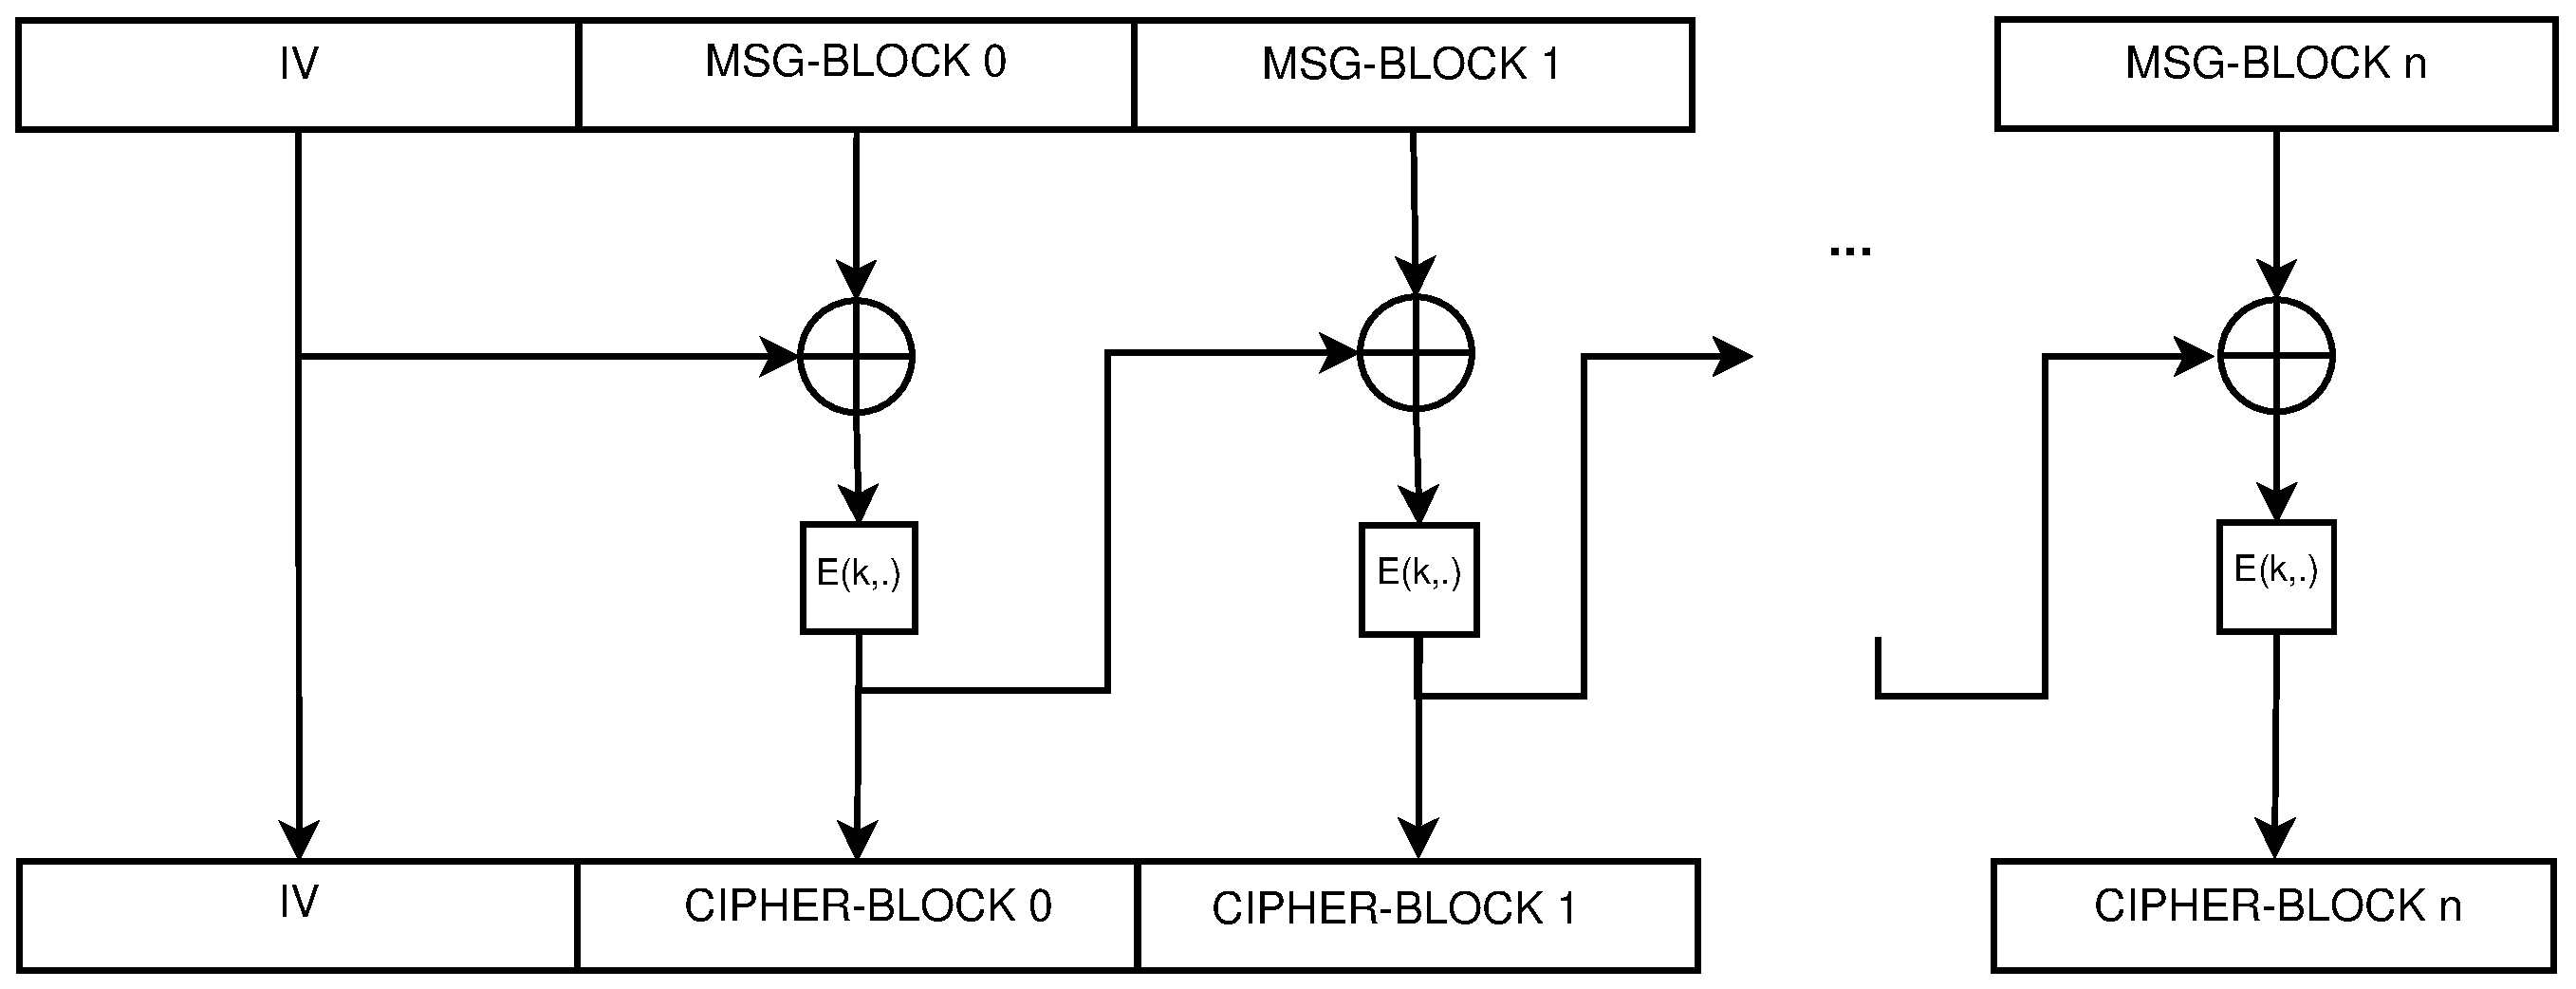
\includegraphics[width=1\textwidth]{figures/CBCencrypt.eps}
    \caption{Cipher Block Chaining for encrypting messages}
    \label{fig:cbc_encrypt}
\end{figure}

\begin{figure}
    \centering
    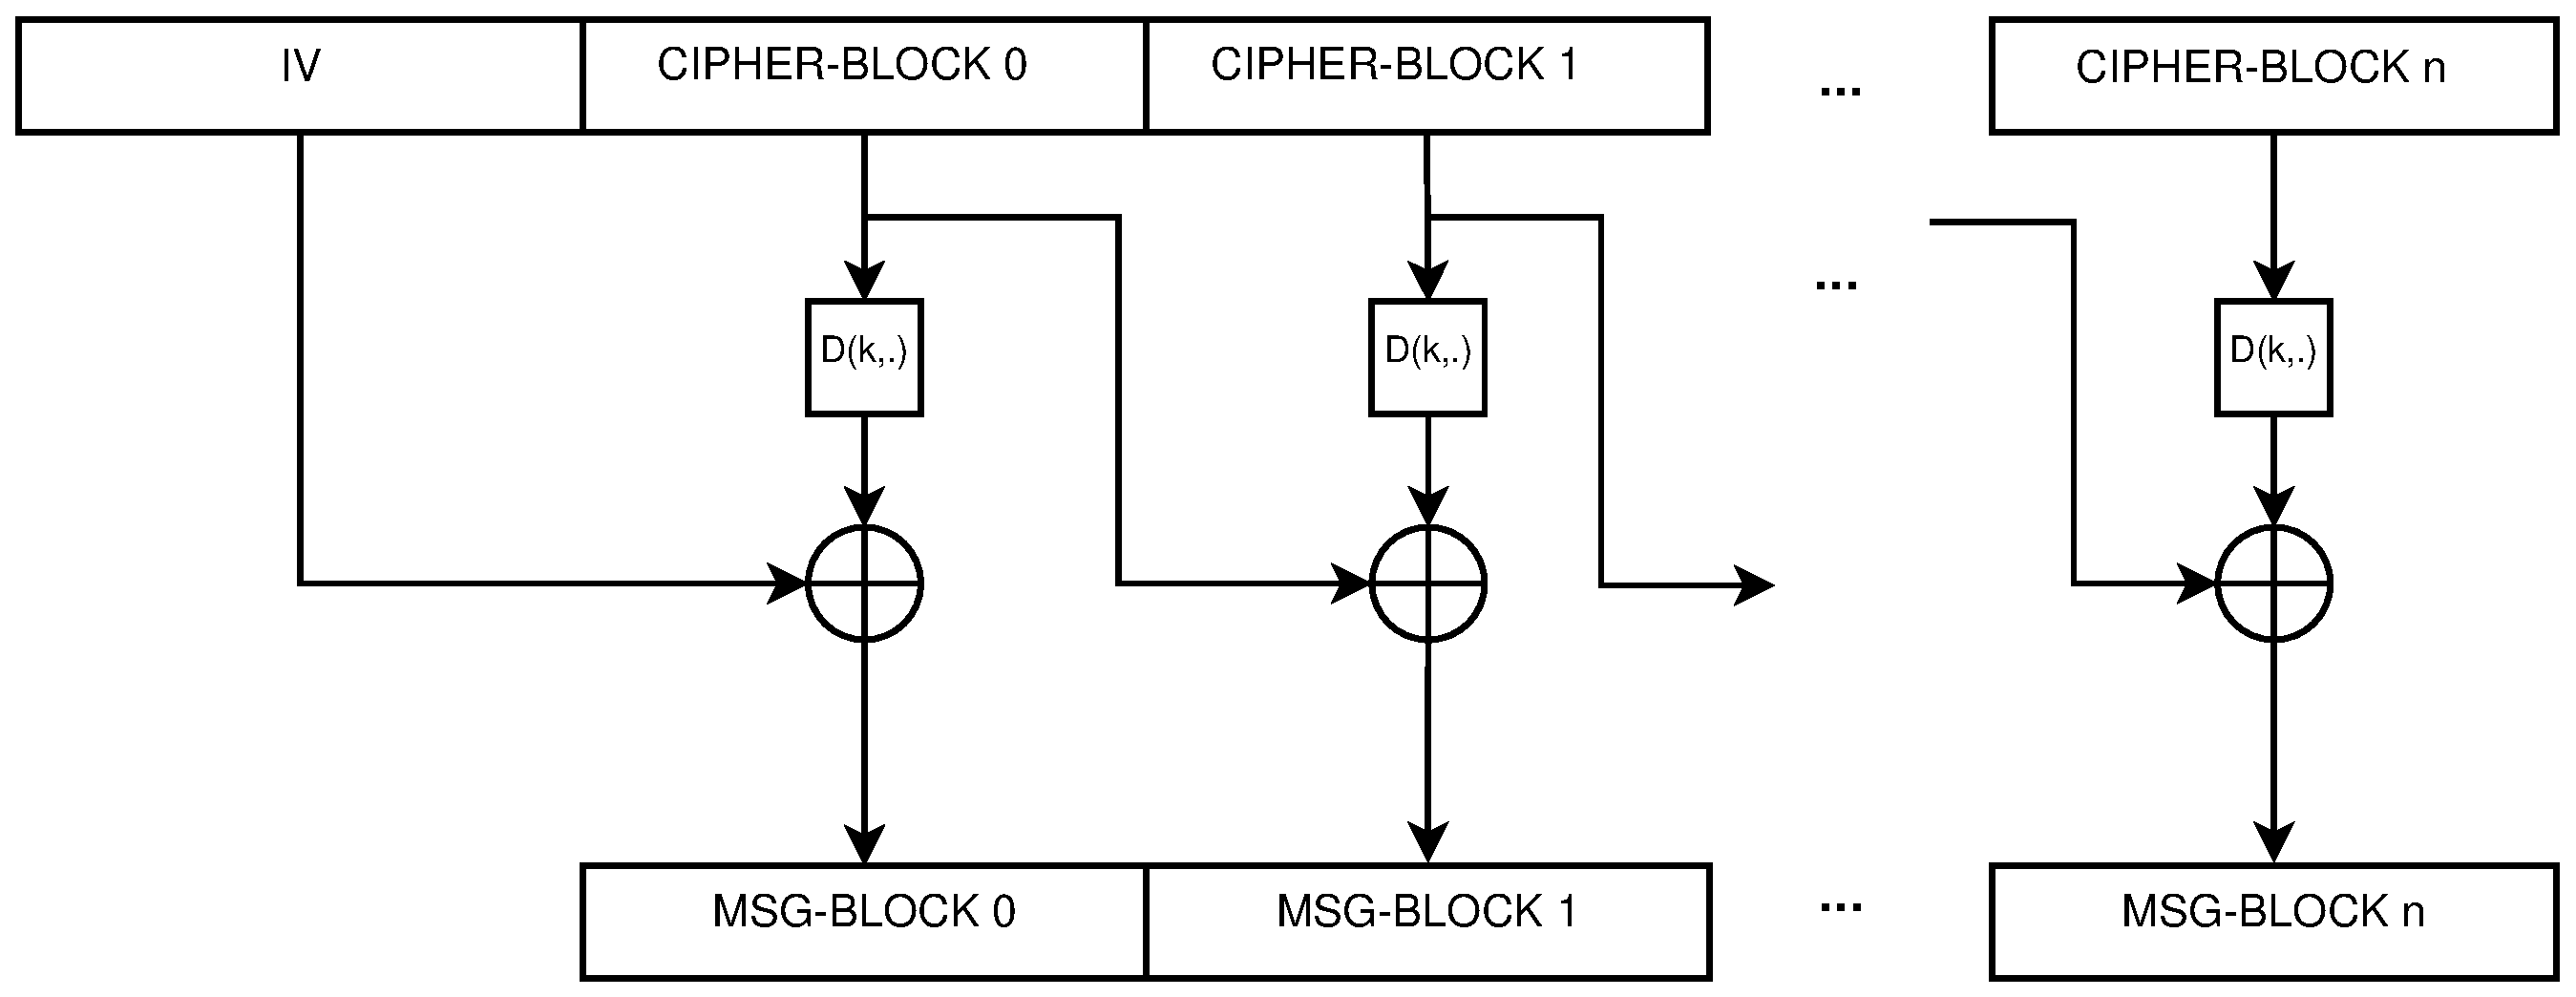
\includegraphics[width=1\textwidth]{figures/CBCdecrypt.eps}
    \caption{Cipher Block Chaining for decrypting messages}
    \label{fig:cbc_decrypt}
\end{figure}

\subsubsection{\gls{ctr}}

This confidentiality mode generates a key stream by encrypting a counter value with a block cipher. The key stream is then applied to the cleartext
blocks with the \gls{xor} operation, as shown in figure \ref{fig:ctr}. For the last block, the key stream is truncated to match the size of the cleartext block.

Decryption works by generating the same key stream on the receiver's side, and applying the \gls{xor} operation to the ciphertext blocks, similar to the
decryption process used in the Vernam cipher.

\begin{figure}
    \centering
    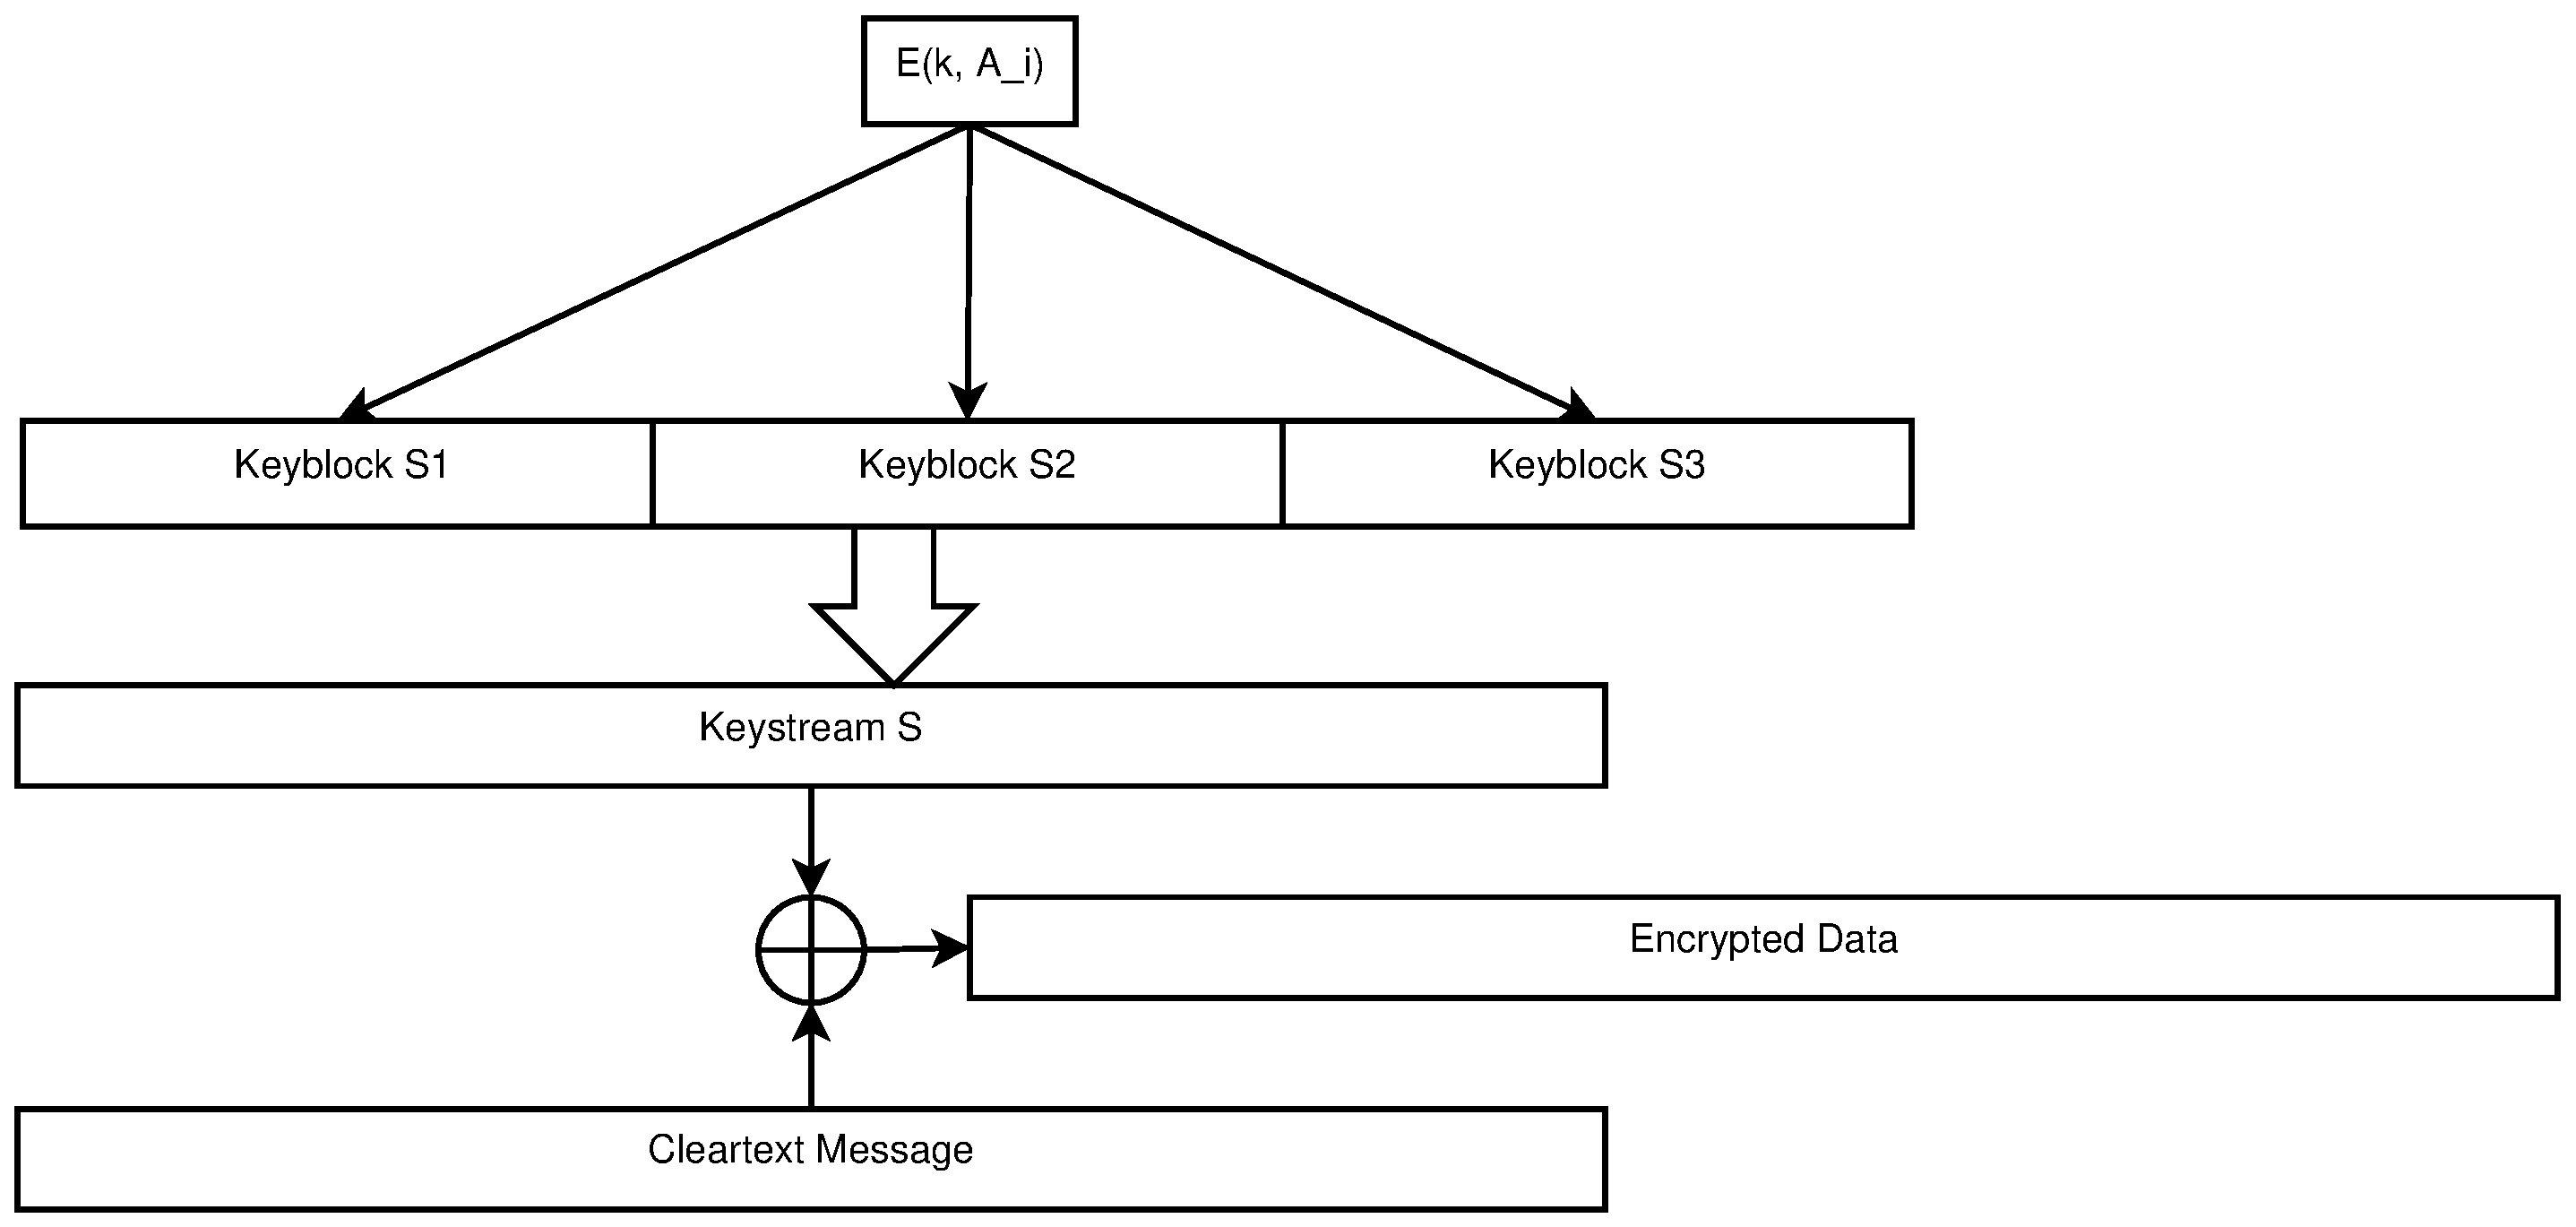
\includegraphics[width=1\textwidth]{figures/CTR.eps}
    \caption{CTR Encryption}
    \label{fig:ctr}
\end{figure}

To avoid the duplicate usage of the same counter value in bidirectional communication, the counter can be combined with a sender-dependent nonce by
concatenation before encrypting the counter:

\begin{center}
 $K_{0} = E(k, nonce || Ctr_0)$\\
 $K_{1} = E(k, nonce || Ctr_1)$\\
 ...\\
 $K_{i} = E(k, nonce || Ctr_i)$\\
 $C_i = K_i \bigoplus M_i$
\end{center}
 
\subsubsection{\gls{cfb}}

\gls{cfb} can be used to turn a block cipher into a stream cipher. Beside the block size $b$, another parameter $s$ determines the operation. $s$ corresponds
to the size of one transmission unit. For initialization, an unpredictable \gls{iv} is set as input for the underlying block cipher. Then, in every
processing step a new transmission unit is generated by \gls{xor}ing the $s$ most significant bits
of the output of the encryption function with the $s$ bit message unit. After that, the \gls{iv} is shifted to the left and the gap is filled
by the newly generated character, as shown in figure \ref{fig:cfb}:
\\
\\
 $C[0] = E(k, IV[0:b-1])[b-1:b-s-1] \bigoplus M[0]$\\
 $C[1] = E(k, IV[0:b-s-1] || C[0])[b-1:b-s-1] \bigoplus M[1]$\\
 ... \\
 $C[n] = E(k, IV[0:b-ns-1] || C[0] || C[1] || .. || C[n-1])[b-1:b-s-1] \bigoplus M[n-1]$\\
\\

To decrypt, the same encryption function, \gls{iv} and key is used to retrieve one transmission unit at a time.
 
\begin{figure}
    \centering
    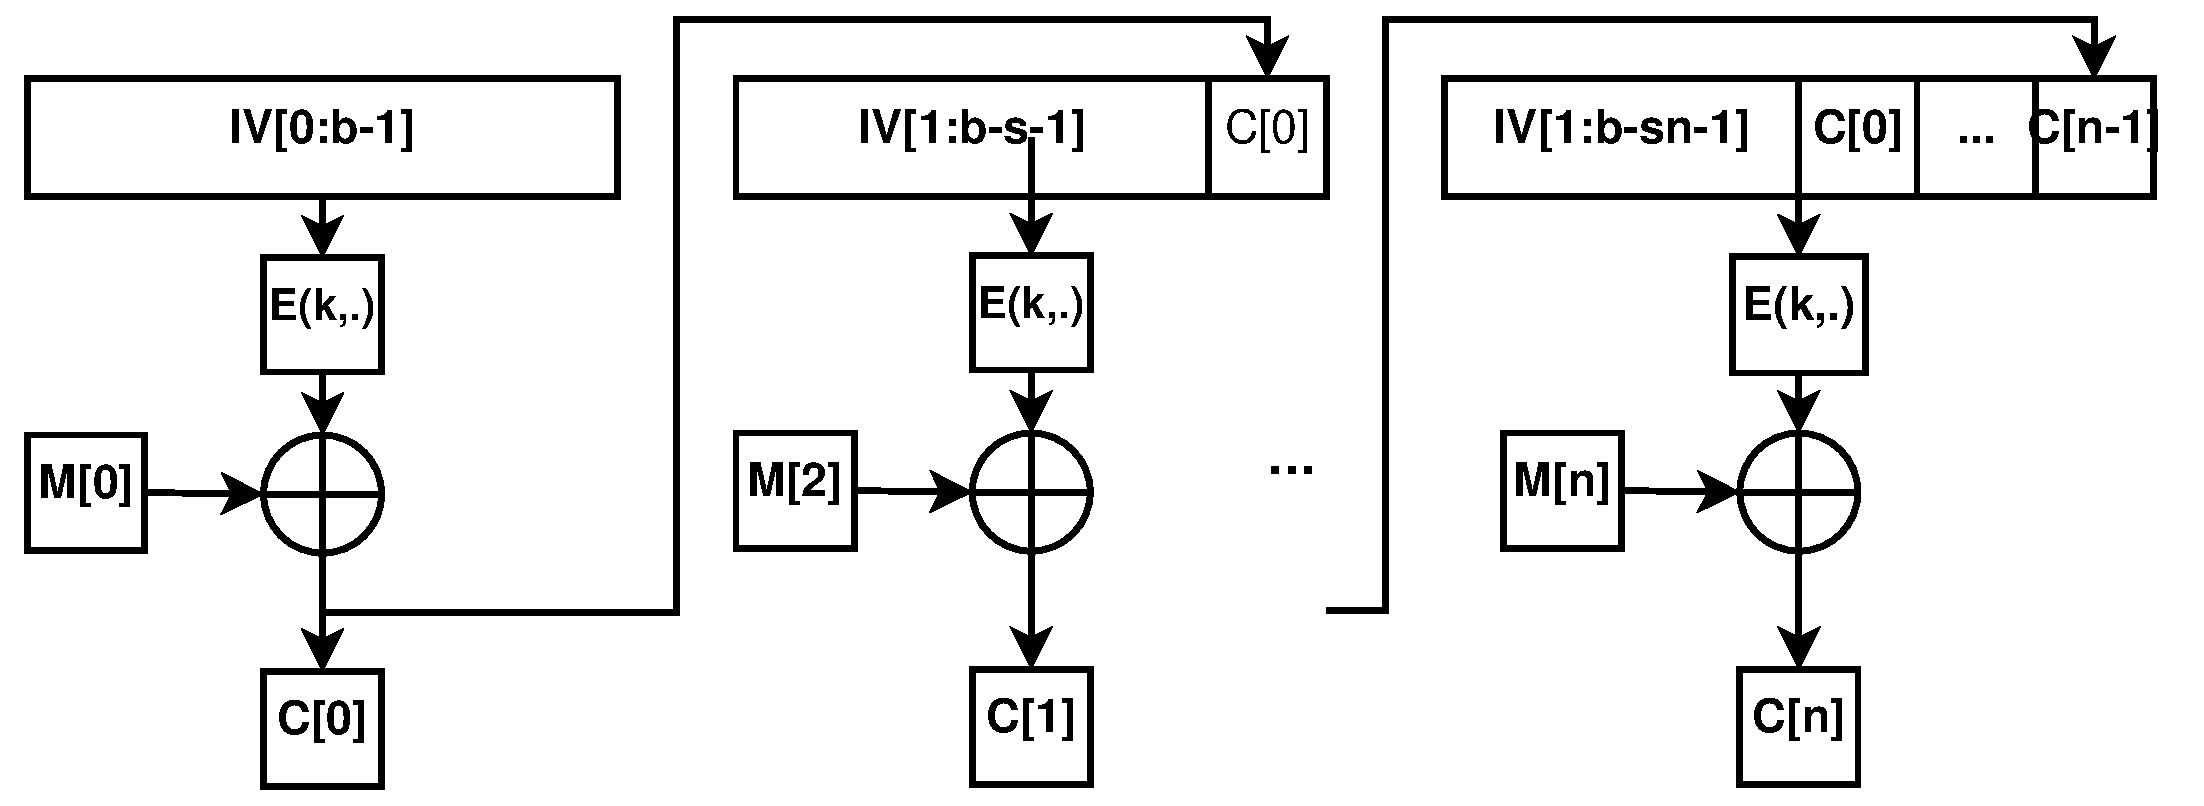
\includegraphics[width=1\textwidth]{figures/CFB.eps}
    \caption{CFB Encryption}
    \label{fig:cfb}
\end{figure}

\subsubsection{\gls{ofb}}

This mode is very similar to \gls{cfb}, but here the $s$ bit output from the encryption function is used directly to update the space caused by the \gls{iv} 
left shift. This avoids error propagation in case a transmission unit was damaged on transmit and thus a bit changed its value:
for \gls{ofb} encryption systems, one or more bit errors in one ciphertext character only affects the decryption of this character. In contrast, one bit error in \gls{cfb} affects
decryption of all following characters.
\\
\\
$O_0 = E(k, IV[0:b-1])[0:s-1]$\\
$C[0] = O_0 \bigoplus M[0]$\\
 $O_1 = E(k, IV[0:b-1] || O_0)[0:s-1]$\\
 $C[1] = O_1 \bigoplus M[1]$\\
 ... \\
 \\
 $0_n = E(k, IV[0:ns-1] || O_0 || O_1 || O_{n-1})[0:s-1]$\\
 $C[n] = O_n \bigoplus M[n]$\\

\begin{figure}
    \centering
    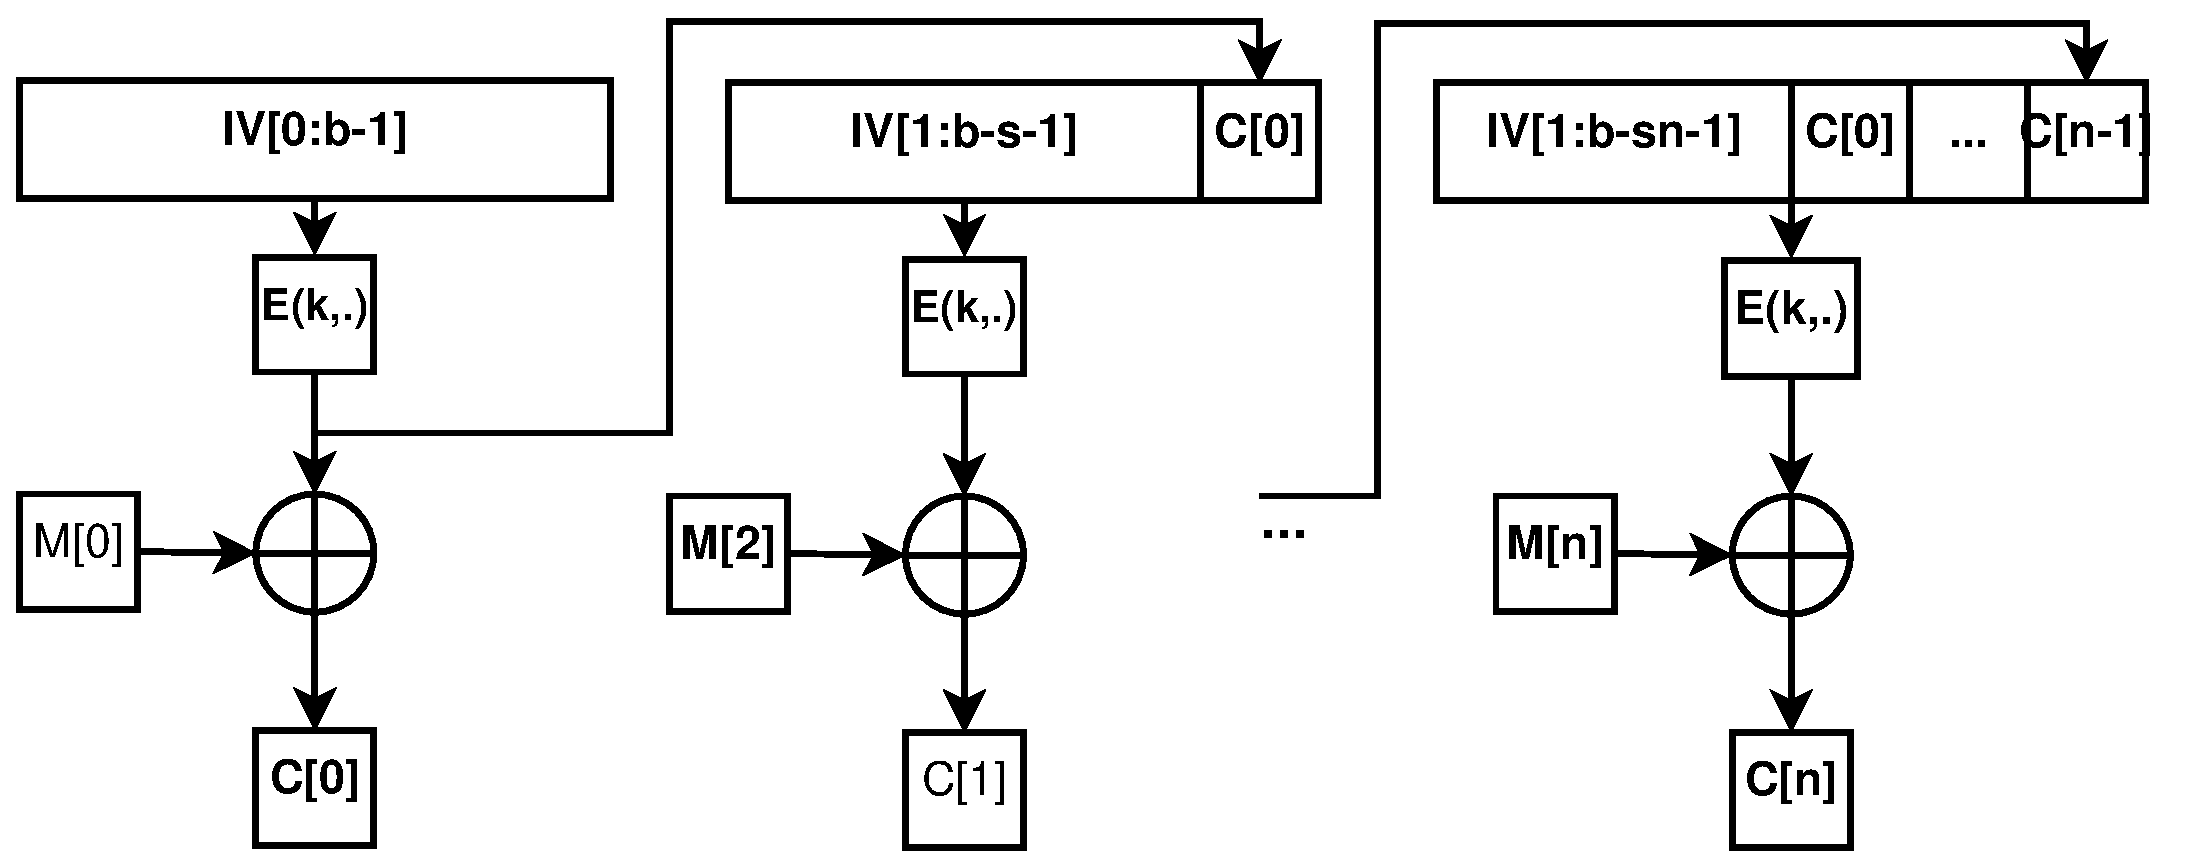
\includegraphics[width=1\textwidth]{figures/OFB.eps}
    \caption{OFB Encryption}
    \label{fig:ofb}
\end{figure}

\subsubsection{Integrity}\label{Integrity}

All modes of operation introduced so far are used to provide confidentiality only. To provide the second column of information security, i.e. integrity, in general
\glspl{mac2} or digital signatures are used.
Digital signatures are based on public key cryptography and are introduced in section \ref{digitalSignatures}. In contrast, \glspl{mac2} use symmetric keys,
providing integrity and authenticity. Integrity means that a data unit is 
protected from tampering by third parties in a way that such a modification by an unauthorized entity is detectable. Authenticity means that the receiver of
a message can verify that the message really was sent from the sender and not by an illegitimate third entity. Obviously, this two concepts are semantically
related: checking the integrity implicitly checks authenticity.
Vice versa, authenticating the sender of a message is only useful if the message itself cannot be modified by an adversary, i.e. integrity is guaranteed. To
avoid confusion, the term integrity is used if the meaning is clear from the context.
\\
\\
In contrast to confidentiality modes, which should always be combined with a method to guarantee integrity (as shown in FIXME), 
integrity-only modes do have a right to exist. For example, archives containing source code for open source project, available from the internet, must not be
encrypted but should be secured against modification. For example, the UNIX based operating system "FreeBSD" uses asymmetric keys to protect it's package
management system from adversary modification.
\\
\\
Combining integrity and confidentiality in a security scheme called \gls{ae} will be handled in section \ref{authEncrypt}.
\\
\\
The basic way to protect a data unit - be it a message traveling from sender to recipient or a file saved for later usage - from modification by a third party is to
generate a tag $t$, also called \gls{mac2}, and concatenating this tag to the message, as shown in figure \ref{fig:tag}.
Verifying the integrity is done by re-generating the tag and comparing it to the saved on. 
\\
\\
As tag generation and tag verification algorithms, keyed or unkeyed cryptographic secure hash functions are used.
For integrity-only, keyed hash functions must be used, or
otherwise an arbitrary entity can modify the message undetectable by regenerating the correct tag. Therefor, a simple checksum like a \gls{crc} or an unkeyed 
hash function can not provide integrity only, simply because the function value can be re-generated by an adversary modifying the message, allowing to mount
an attacker called \gls{mac2} forgery.
Nevertheless, in combination with a confidentiality mode such an unkeyed function \textit{may} be secure, although it's use is discouraged because many applications operating
this way are broken and can be attacked (i.e. \gls{ssh} version 1 \cite{zalewskissh}).
\\
\\
A hash functions takes as input an arbitrary large message $\mathcal{M}$ and generates a hash value $t = h(\mathcal{M})$ of fixed size, therefor $|M| >> |t|$. This many-to-one
mapping implies the existence of collisions, i.e. the existence of distinct messages $m_1, m_2$ which are mapped to the same tag $t$.
\begin{figure}
    \centering
    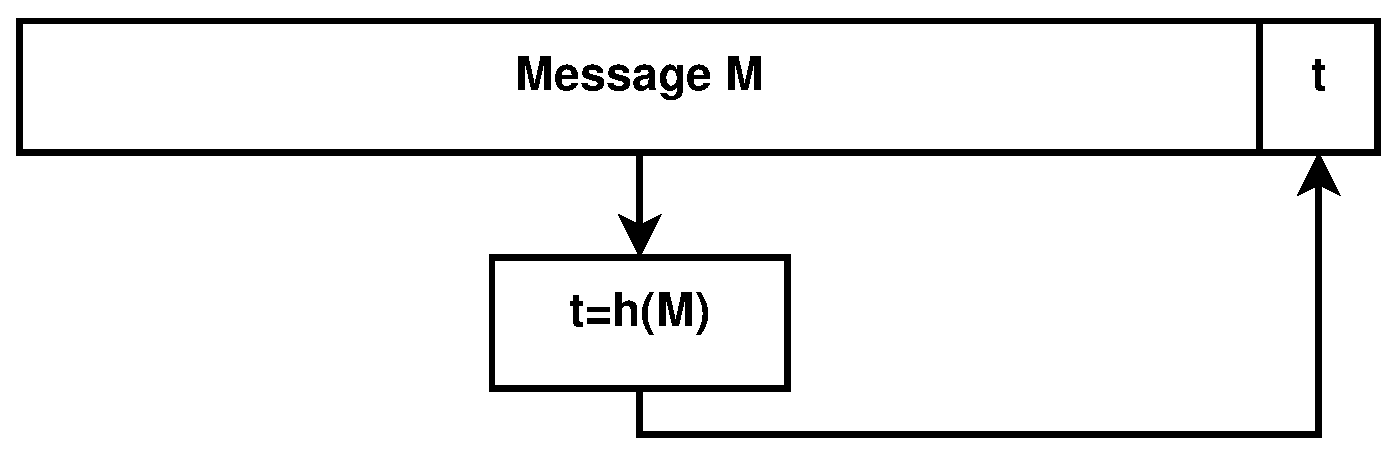
\includegraphics[width=0.5\textwidth]{figures/tag.eps}
    \caption{Tag generation}
    \label{fig:tag}
\end{figure}
\\
To be cryptographically secure, a hash function must fulfill specific properties \cite{6732428}: firstly, while it should be easy to generate the tag
by calculating $t = h(m)$, reversing the process to get $m$ by executing $h(t)^{-1}$ should be hard, a property called \textit{preimage resistance}. 
Additionally, \textit{2nd-preimage resistance} assures that for any given message $m$ and corresponding tag $t$, it must be infeasible to find a second message
that maps to the same tag. Finally, \textit{(strong) collision resistance} states that it also must be infeasible to find any two messages generating
the same tag, therefore collision resistance implies 2nd-preimage resistance \cite{handbookCR}.
\\
Important representatives of cryptographically secure hash functions are the family of \glspl{sha}, with variants providing hashes of 128, 256, 384 or 512 bit 
length, defined by \gls{nist} \cite{nistSHA}.
\\
Because these hash functions lack a secret key and therefor would allow \gls{mac2} forgery, a construction called \gls{hmac} can be used, which takes 
additionally to the message $m$ as input a key $k$, and $ipad$ and $opad$ being constant values \cite{hmac}.

\begin{align}
 t = S(k, m) = h((k \bigoplus opad) || h((k \bigoplus ipad) || m)) 
\end{align}
\\
\\
A different way for tag-generation, called \gls{cbc}-\gls{mac2}, is based on block ciphers, utilizing a construction similar to \gls{cbc} mode encryption,
shown in figure \ref{fig:cbc_MAC}.

\begin{figure}\label{cbcMAC}
    \centering
    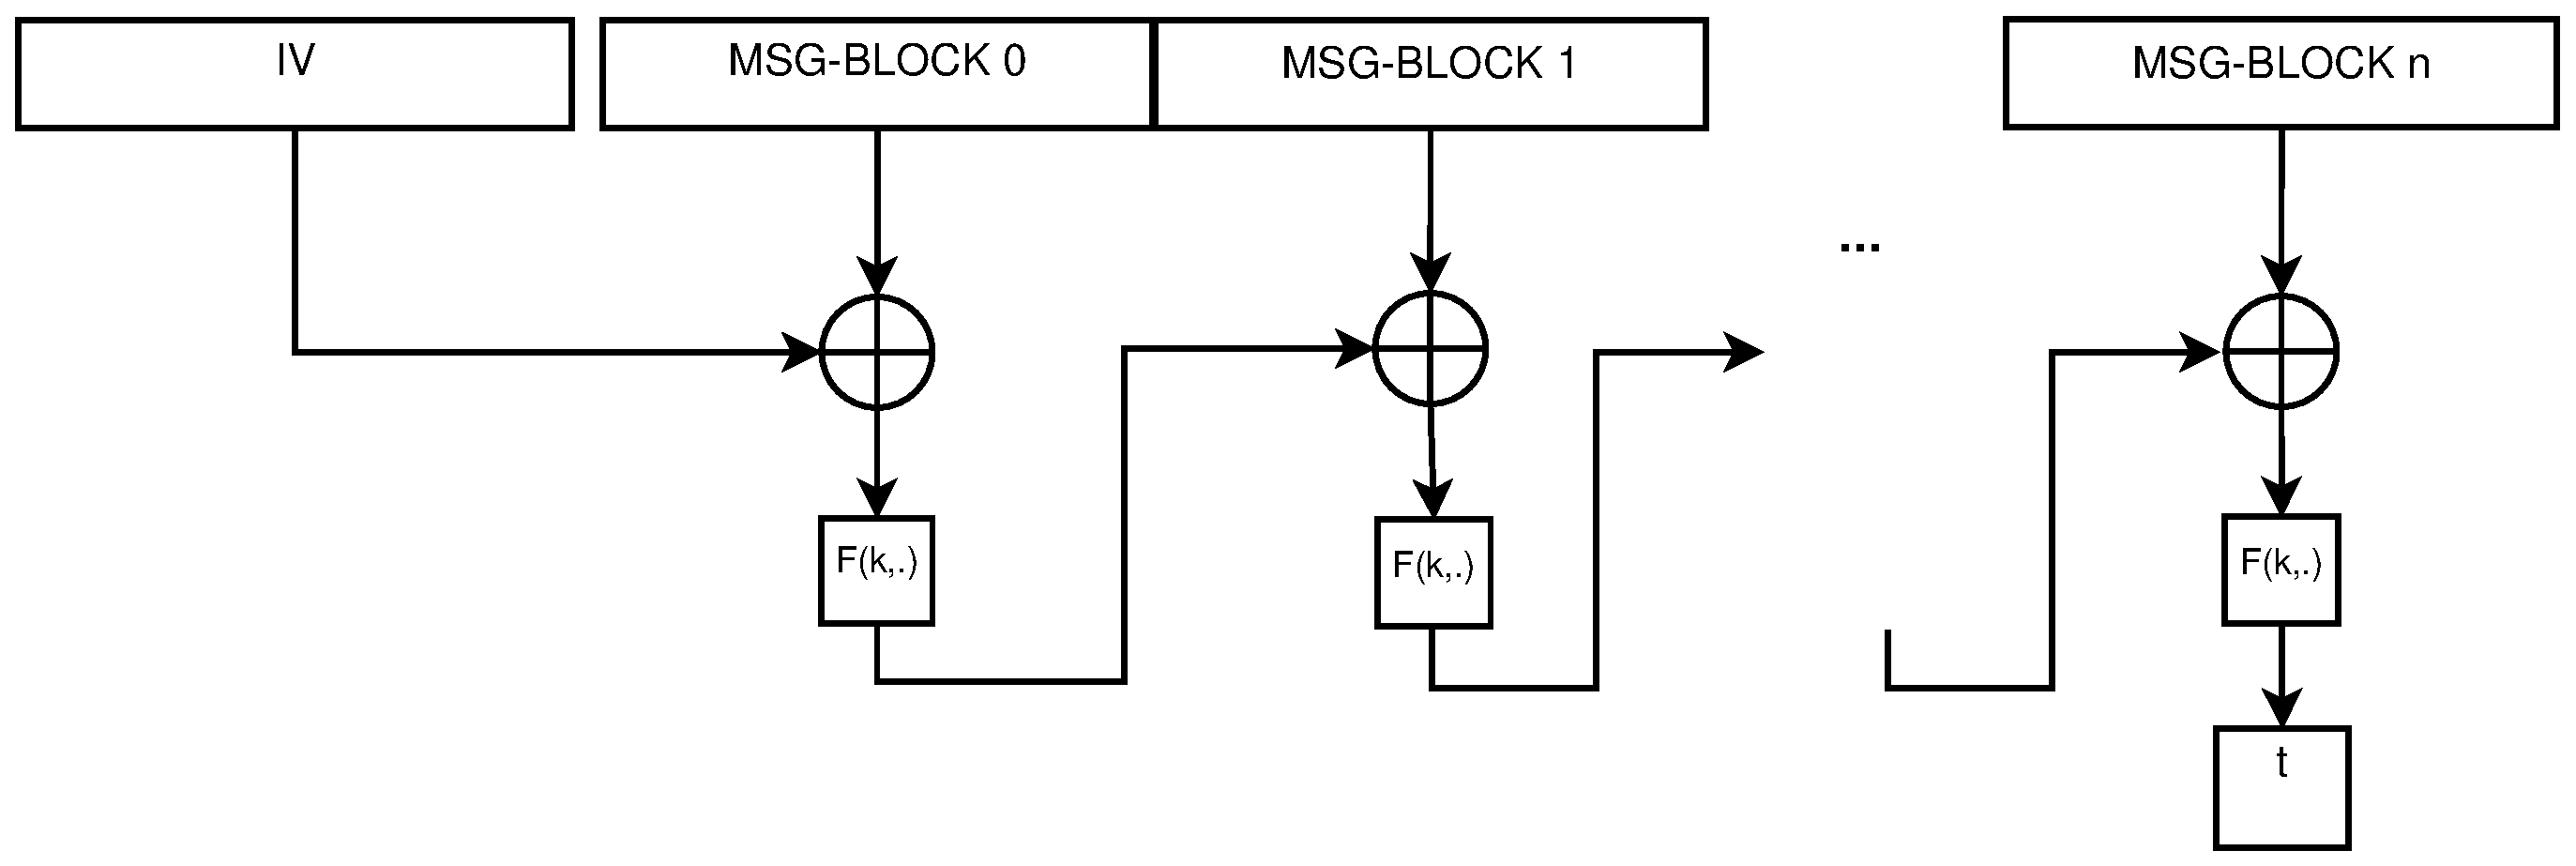
\includegraphics[width=1\textwidth]{figures/CBCMac.eps}
    \caption{Cipher Block Chaining for generating a MAC}
    \label{fig:cbc_MAC}
\end{figure}

\begin{figure}\label{cbcMACFlags}
    \centering
    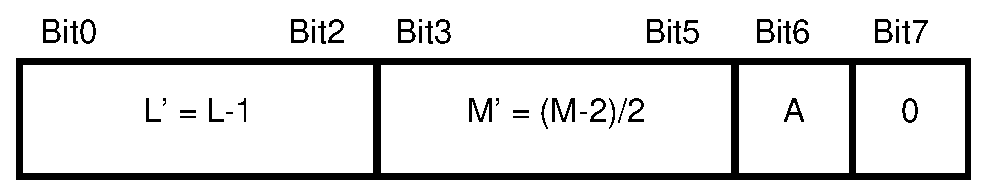
\includegraphics[width=0.5\textwidth]{figures/CBCIVFlags.eps}
    \caption{Flag Field of CBC IV}
    \label{fig:cbc_Flags}
\end{figure}

\subsection{Key lenghts}

\cite{Lenstra04keylength}

\section{Authenticated Encryption}\label{authEncrypt}

\subsection{CCM}

CCM\footnote{http://tools.ietf.org/html/rfc3610}, short for \textit{Counter with CBC-MAC} combines CBC for authentication and CTR mode for encryption.
CBC generates the MAC for the message first, appends this MAC to the cleartext data and afterwards encrypts data + MAC with counter mode, thus using a
\textit{MAC-then-Encrypt} scheme. The only
supported block size is 128-bit blocks, so it is possible, but not mandatory, to use 128-bit AES as underlying block cipher.
\\
Two application dependent parameters have to be fixed first: 
\begin{itemize}
 \item M: Number of octets in the MAC field. A shorter MAC obviously means less overhead, but it also makes it easier for an adversary to guess the correct
 value of a MAC, so valid values are $M \in \{4, 6, 8, 10, 12, 14, 16\}$. FIXME: shorter MACs insecure, border=4 ? 
 \item L: Number of octets in the length field. This is a trade-off between the maximum message size and the size of the nonce. Valid values are $2 \leq L \leq 18$.
 For example, when setting $L = 2$, 2 bytes are reserved for the length field, which means that the biggest message that can be encrypted is of size 64kB. The actual
 length of the message is filled into the field named 'length(msg)', as shown in figure \ref{fig:cbc_MAC}.
\end{itemize}

Both parameters are encoded in the very first byte of the first message block, thus reducing the possible maxium size of the nounce, as shown in figure \ref{fig:cbc_Flags}.
Bit 6 of the length field is set to 1 if additional authenicated data(FIXME) are sent, and bit 7 is reserved and set to 0.


\subsubsection{Generating the MAC}

As shown in chapter \ref{authenticity} in figure\ref{fig:cbc_MAC}, the first message block $M_0$ is \gls{xor}'d with a nonce or initialization vector(IV, see figure
\ref{fig:ccrMacIV}), which \textbf{must be unique per key}.FIXME
The result of the \gls{xor} operation is then feed to the block-cipher to get the first cipherblock $C_0$. The encrypted data $C_0$ gets \gls{xor}'d with the next message block $M_1$, and this
result becomes the input for the block cipher, and so on, iterating over all $n$ message blocks to determine the tag $t$:

\begin{figure}
    \centering
    \includegraphics[width=0.5\textwidth]{figures/"CCM CBC IV".png}
    \caption{IV for CBC MAC}
    \label{fig:ccrMacIV}
\end{figure}


\begin{center}
 $C_0 = F(k, M_0 \bigoplus IV )$
 \\
 $C_1 = F(k, M_1 \bigoplus C_1) $
 \\
 $...$
 \\
 $C_n = F(k, M_n \bigoplus C_{(n-1)})$
 \\
\end{center}

The resulting tag $t$ can be truncated, corresponding to the chosen MAC size $M$:
\begin{center}
  $t = C_n[M:0]$, with $M \in \{4, 6, 8, 10, 12, 14, 16\}$
\end{center}
which means that the tag $t$ consists of the least significant $M$ bytes of the output of the last encryption block.

\subsubsection{Encrypting Data and MAC}

Counter-mode is used for encrypting the actual payload and the concatenated, CBC mode generated MAC.
Thus, authenticated encryption is achieved in a manner also called 'mac-then-encrypt'. While authenticated
encryption modes implementing this ordering(generate mac first, then encrypt data and mac) \textit{may}
be vulnerable to padding oracle attacks(FIXME), counter mode effectively avoids these simply because
there is no padding needed, as will be shown.

Counter mode implements a weaker form of the one time pad by generating a keystream of sufficient
length, and then applying the \gls{xor} operation to the keystream and the data, as shown in figure \ref{fig:ctr}.


First, keyblocks with 16 byte length each are generated by encrypting the nounce, a flag and a counter with the key. These 
keyblocks are then concatenated and trimmed to the proper length(=length of the message to encrypt). This obtained keystream
is then bitwise \gls{xor}'ed with the cleartextmessage(which consists of the data and the MAC), yielding the final encryption.


\section{Public Key Cryptography}

Public Key Cryptography solves the problem of establishing a secure channel by using an insecure one.
Here sender and recipient use two different keys: one for encryption, called \textit{public key}, the other
for decryption, called \textit{private key}. This key pair belongs together, hence this scheme is also called \textit{asymmetric} encryption. A fundamental requirement
is that it must be hard
to derive the decryption key from the encryption key. This behavior is achieved by some kind of public known one-way function where it is computationally
easy to calculate the result of $f(x) = y$, but only given $y$, it is computationally - in the domain of processing power and/or memory - hard
to reverse this function to get $x$.
The basic idea for such a one-way function was formulated for the first time in the year 1874 by William Stanley Jevons stating:
\\
\\
\textit{"Can the reader say what two numbers multiplied together will produce the number 8616460799? I think it unlikely that anyone but myself will
ever know."} \cite{wStanley} 
\\
\\
Although his statement was not related to cryptography at all, and of course factoring of much bigger numbers is doable nowadays, this statement exactly describes
the spirit of public key systems, and the security of RSA, introduced below, is directly connected to the inability to factor large numbers in reasonable time.

Because disclosure of the public key does not affect the security of the scheme, the public key can be published in some sort of dictionary.
An entity wanting to send an encrypted message to a receiver can then look up the receiver's public key, encrypt the message and send the resulting
ciphertext to the recipient, who then can decrypt the message. 
\\
\\
It is remarkable that any algorithm establishing public keys must authenticate it's  participants, or it will be vulnerable to man-in-the-middle attacks.

\subsection{Merkle Puzzles}

In \cite{Merkle}, Ralph C. Merkle developed an algorithm for key exchange between two parties. While the algorithm is based on symmetric ciphers and is
not practicable, it motivates the usage of public key systems based on algebraic structures and is therefor introduced.
\\
\\
The key idea is that the necessary work by the two legitimate parties when negotiating a key is bounded by $O(n)$, while an adversary must spend $O(n^2)$ to 
also calculate the key, thus generating a quadratic gap. 
Merkle defines a puzzle as cipher text that is supposed to be broken. This can be achieved by restricting the size of the symmetric key used such that an
exhaustive search can be finished in feasible time. Every puzzle contains an id and a session key, booth chosen randomly, as well as a static string,
known to all participants.

The party initiating the key exchange, called $X$, generates $n$ such puzzles and sends all of them to the receiver $Y$. $Y$ picks one puzzle at random and
decrypts it by trying all possible keys. Because of the static string inside the puzzle, $Y$ knows for sure when the correct key has been tried.
$Y$ then extracts the session key and sends the corresponding id back to $X$. Subsequently, booth parties can use the session key referenced by the id for encryption.
An eavesdropper $Z$, monitoring all puzzles, cannot directly determine which of them is containing the returned id and therefor does not know the session key the 
two parties agreed on - the only possibility for $Z$ is to attack \textbf{all} puzzles, squaring the effort spent by $X$ and $Y$.
\\

If, for example, every puzzle can be broken by $2^{32}$ computations, and $2^{32}$ different puzzles are used, $X$ must prepare, save and send $2^{32}$ puzzles
to $Y$, who in turn must try $2^{32}$ different keys. $Z$ must crack all $2^{32}$ puzzles, each with effort $2^{32}$, thus resulting in $2^{64}$ processing steps.
\\

While this algorithm is very wasteful in regards of processing power, memory and communication capacity, such a protocol would be useful if a more-than-quadratic
blowup could be achieved, but unfortunately, for all algorithms based on symmetric ciphers, this quadratic gap is the best that can be achieved,
as shown in \cite{Barak09merklepuzzles}.   
\\
 
To further increase the effort an attacker has to spend a different approach has to be found. It turns out that hard mathematical problems exist that are 
suitable for such a purpose. 
Therefor, in the next sections three important public key algorithms are introduced: \gls{dh} key exchange, based on prime fields, \gls{ecc}, and RSA.
The former 2 of them are based on finite fields, therefore a short mathematical introduction is given first.

\subsubsection{Finite Fields}\label{finiteFields}

A field consists of a set $\mathcal{F}$ together with two operations $\cdot$, namely addition "+" and multiplication "*", satisfying the following properties:

\begin{itemize}
 \item  Closure: for all elements from $\mathcal{F}$, the set is closed under the defined operations, i.e. applying an operator $\cdot$ to two elements from the set results in an
element also belonging to the set.
 \item Associativity and Commutativity hold, i.e. $a \cdot (b \cdot c) = (a \cdot b) \cdot c$ and $a \cdot b = b \cdot a$
 \item For both operations and all elements from the set $\mathcal{F}$ an identity element $e$ exists s.t. $a\cdot e = a$
 \item For both operations and all elements from the set $\mathcal{F} \backslash \{0\}$ an inverse element exists s.t. $a\cdot a^{-1} = e$
 \item Distributivity holds: $(a+b) \cdot c = a \cdot c + b \cdot c$ for all elements 
\end{itemize}

For a finite field, the size of the set 
$\mathcal{F}$ is finite and called \textit{order} of the field, with the identities "0" for addition and "1" for
multiplication. Inverses can be found to for all
elements regarding addition s.t. $a + (-a) = e = 0$ and regarding multiplication for all elements except ${0}$ s.t. $a * a^{-1} = e = 1$.
\\
\\
A specific example of a finite field is a prime file, which can be constructed by taking the set of integers $\mathbb{Z}\pmod p$, with $p \in \mathbb{P}$, thus
restricting the set of all integers to the set $\mathbb{Z}_p = \{0, 1, ..., p-1\}$.
By choosing $p$ as prime it is ensured that for any element $a \in \mathcal{F} \backslash\{0\}$, a multiplicative inverse exists: $ a * a^{-1} = 1 \pmod p$.
The set of numbers for which multiplicative inverses exist is called $\mathbb{Z}{_p}^*$, so for $p$ being prime, $\mathbb{Z}_p \backslash \{0\} = \mathbb{Z}{_p}^*$.
\\

By raising an element $a \in \mathbb{Z}_p$ to different powers, a subgroup of $\mathbb{Z}{_p}^*$
is generated, a fact that follows from Fermat's little theorem stating that for $p$ being prime and raising $a$ to the power $p-1$, the outcome is congruent 1
modulo p:
\begin{center}
 $a^{p-1} \equiv 1 \pmod p $ \\
\end{center}
Raising $a$ to higher powers results in:
\\
\\
 $a^{p} \equiv a*a^{p-1} \equiv a \pmod p$ \\
 ... \\
 $a^{2p} \equiv a^2 * a^{p-1} * a^{p-1} \equiv a^2 \pmod p$ 
\\
\\
Thus, generating higher powers than $(p-1)$ does not yield different outcomes. If by raising $a$ to $(p-1)$ different powers all elements from $\mathbb{Z}{_p}^*$ can
be generated, $a$ is called \textit{primitive root} or \textit{generator}, generating a cyclic group.
If $p$ is prime it can be shown that at least one such generator $g$ must exist and can be found efficiently \cite{primitiveRoot}.
Conversely this means that for all elements from  $\mathbb{Z}{_p}^*$ a unique exponent in the interval $[0, p-1]$ exists,
called the \textit{discrete logarithm for the base $ g \pmod p$}.

To find
the discrete logarithm, several algorithms exist. The most naive method conducts an exhaustive search, so for a prime of $n$ bits length, $2^n$ search operations
are necessary. More efficient algorithms exist, with the best methods finishing after about $2^{\frac{n}{2}}$ steps \cite{5199978}. 
Therefore, by choosing a sufficient large prime, finding the discrete logarithm is considered a hard problem, a fact
that is exploited by the \gls{dh} key exchange algorithm.

\subsection{\gls{dh} Key-Exchange}

Whitfield Diffie and Martin Hellman proposed a way to solve the problem for key-exchange based on finite fields
when they published their paper \textit{New Directions in Cryptography} in the year 1976 \cite{1055638}. The algorithm enables two entities to agree on a 
shared secret which never has to be transmitted between them. The security of their original algorithm
is based on the hardness of the \textit{Discrete Logarithm Problem}.

With the original \gls{dh} algorithm, 2 entities - $A$ and $B$ - use exponentiation over finite fields to agree on a shared secret, which
then can be used parametrize a block or stream cipher. The first step for booth entities is to agree on the set of parameters $\{p, q, g\}$, where $p$ is a 
large prime, $q$ is a prime divisor of $p-1$, and $g$ is a generator of the cyclic group ${Z_p}^*$ in the range $[1, p-1]$. These parameters are not secret and
can thus be sent over an unsecured channel.
Additionally, each entity randomly chooses an integer $x$ from the interval $[1, q-2]$, and calculates the value $y = g^x \pmod p$. $x$ is the private key,
$y$, which is computationally easy to calculate, is the public key. $A$ sends its public key $y_A \equiv g^{x_A} \pmod p$ to $B$, and $B$ its public key
$y_B \equiv g^{x_B} \pmod p$ to $A$. Due to the characteristics of exponentiation, $A$ and $B$ can now easily derive the shared secret by using its counterpart's
public key and raising it to the power of it's own private key in the domain of ${Z_p}^*$:

\begin{center}
 $k_B \equiv {y_A}^{x_B} \equiv (g^{x_A})^{x_B} \equiv g^{x_A*x_B} \pmod p $\\
 $ = $ \\
 $ k_A \equiv {y_B}^{x_A} \equiv g(^{x_B})^{x_A} \equiv g^{x_B*x_A} \pmod p $
\end{center}
An eavesdropper that intercepts the initially sent parameter set $\{p, g, q\}$ and the public keys $y_A$ and $y_B$ and that wants to calculate the shared secret
$k_A = K_B$  must therefore calculate the discrete logarithm of $y_A$ or $y_B$ to the base $p$, i.e. must solve the \gls{dlp}, a hard problem as shown in
section \ref{finiteFields}.
\\

% FIXME: EL GAMAL scheme vorstellen??


\subsection{\gls{ecdh}}

The \gls{dh} protocol can be based on different kinds of cyclic groups. Koblitz and Miller independently proposed the usage of cyclic groups based on
\glspl{ec} \cite{eccKoblitz} \cite{eccMiller}.
This cyclic groups are receiving increased importance in cryptography because they allow the usage
of shorter keys compared to \gls{dh} over prime fields or RSA, while providing the same level of secrecy.

An \gls{ec} is basically the set of all points
satisfying an equation with the form as shown in \ref{basicEC}:

\begin{align}\label{basicEC}
 y^2 = x^3 + ax +b
\end{align}

\begin{minipage}{\linewidth}
 %     \centering
      \begin{minipage}{0.5\linewidth}
          \begin{figure}[H]
              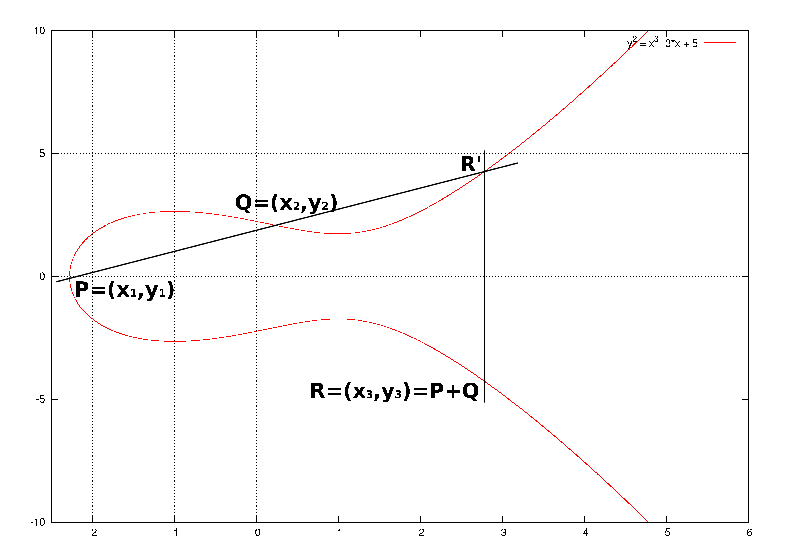
\includegraphics[width=\linewidth]{figures/ecAdd.eps}
              \caption{Adding two points}
              \label{fig:ecAdd}
          \end{figure}
      \end{minipage}
     % \hspace{0.05\linewidth}
      \begin{minipage}{0.5\linewidth}
          \begin{figure}[H]
              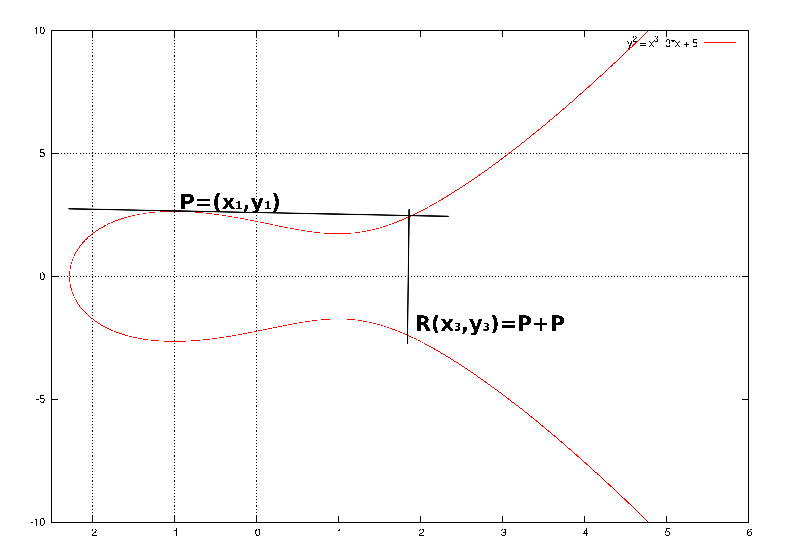
\includegraphics[width=\linewidth]{figures/doubleEC.eps}
              \caption{Doubling a point}
              \label{fig:ecDouble}
          \end{figure}
      \end{minipage}
  \end{minipage}

By defining an \gls{ec} over $\mathbb{Z}_p$, with $a, b \in \mathbb{Z}_p$, a cyclic group can be generated. The addition operation that "adds" two points on
this curve is defined by a "chord-and-tangent" rule. Figure \ref{fig:ecAdd}
shows addition of two points, while \ref{fig:ecDouble} shows adding a point to itself. It is important to note that this representation is shown in the domain
$\mathbb{R}$ for visualization - in real \gls{ec} cryptography, only elements from $\mathbb{Z}_p$ are allowed. Addition is defined as connecting points $A$ and 
$Q$, finding the intersection of the line with the \gls{ec} ($R'$) and reflecting that point across the x-axis to obtain the result $R$.
Point-doubling of $P$ is achieved in a similar way by determining the tangent of $P$, finding the intersection and reflection. Formulae to calculate x- and y-coordinates for the resulting points
for point addition $R=P+Q$ and point doubling $R=P+P$ are shown in equations \ref{adding} and \ref{doubling} respectively:

\begin{align}\label{adding}
 x_3 = (\frac{y_2-y_1}{x_2-x_1})^2-x_1-x_2, y_3=\frac{y_2-y_1}{x_2-x_1}(x_1-x_3)-y_1
\end{align}

\begin{align}\label{doubling}
 x_3 = (\frac{3x_1^2 +a}{2y_1})^2 - 2x_1, y_3=\frac{3x_1^2+a}{2y_1}(x_1-x_3)-y_1
\end{align}

Multiplication is defined as successive addition of a point to it self in the way

\begin{center}
 $kP = \underbrace{P+P+...+P}_{k-times}$
\end{center}

An imaginary point "in infinity", denoted $\infty$, serves as additive neutral element, and also belongs to the \gls{ec} by definition:

\begin{center}
 $P + \infty = \infty + P = P$
\end{center}

Negatives can be calculated easily due to the symmetric nature of the curves by swapping the sign of the y-coordinate of the point. For point $P$ with coordinates $(x, y)$, $-P$ is defined as
$(x,-y)$, thus satisfying $P + (-P) = \infty$.
\\
\\
With these prerequisites, the \gls{ecdlp} \cite{ecdlp} can be defined as following: given an \gls{ec} $E$ over the finite field $\mathcal{F}_p$ and 2 points $P,Q$ on this curve, %FIXME: "P of order n...???"
find the integer $k$ s.t. $Q = kP$. $k$ is called the discrete logarithm of $Q$ to the base $P$.
\\
To build a public key system, two users $A$ and $B$ initially agree on a set of public parameters, called \textit{domain parameters}, including a representation
of the curve and a point $P$ belonging to the curve, called \textit{base point}. Then $A$ selects a randomly chosen integer $k_A$, calculates $P_A = k_A*P$ and sends
this point to $B$, who in turn randomly chooses $k_B$ and sends $P_B = k_B*P$ to $A$. Subsequently, booth can calculate the point $k_A*k_B*P$, which can be used
to derive a key.

\subsection{RSA}

RSA, published in 1977 by Ron Rivest, Adi Shamir, and Leonard Adleman \cite{RSA} and formalized in \cite{pkcs1},
relies on the hardness of finding the prime factors of a big composite number.
In contrast to \gls{dh}, RSA is not directly connected to key negotiation, but can instead be used to encrypt \textit{and} sign messages. 

For key generation, 
two large primes $p, q$, which should be of about same size, are chosen randomly, with $N = pq$. Additionally, a public exponent $e$ and a private exponent
$d$ are chosen s.t. they are multiplicative inverses to each other in $\pmod{\varphi(N)}$:
\begin{align}\label{ed}
 e * d \equiv 1 \pmod {\varphi(N)}
\end{align}
$\varphi(N)$, Euler's totient function, counts the number of integers in the interval $[1, N]$ which are relatively prime to $N$.
For a prime $p$, $\varphi(p) = (p-1)$, therefore for the product
$p*q$ of two different primes, $\varphi(p*q) = (p-1) * (q-1)$.
Additionally, Euler's theorem is used:
\begin{align}\label{euler}
a^{\varphi(N)} \equiv 1 \pmod N
\end{align}
The public key consists of the pair
\begin{center}
 $(N, e)$
\end{center}
and the private key of the pair
\begin{center}
 $(N, d)$
\end{center}

In practice, for the public exponent $e$ the numbers 3, 5, 17, 257 or 65537 are suggested \cite{891000}, a suitable $d$ satisfying \ref{ed} can then be found
by using the extended Euclidean algorithm.

\subsubsection{Encrypting of messages}

To encrypt, the message $M$ must be converted to an integer. Then, the sender uses the recipients public key and raises $M$ to the power of $e \pmod N$:
\begin{center}
 $C \equiv M^e \pmod N$
\end{center}
To decrypt, the receiver uses his own private key to raise $C$ to the power of $d \pmod N$:
\begin{align}\label{decrypt}
 M' \equiv C^d \equiv M^{d*e} \bmod N
\end{align}
From the way $e$ and $d$ have been chosen in \ref{ed} it follows that 
\begin{align}\label{ed2}
 e*d = k * \varphi(N) + 1, k \in \mathbb{Z} 
\end{align}
Inserting \ref{ed2} in equation \ref{decrypt} yields:
\begin{align}\label{cong}
  M' \equiv M^{k * \varphi(N) + 1} \equiv M* M^{k * \varphi(N)} \pmod N
\end{align}
By using Euler's theorem \ref{euler}, expression \ref{cong} shows that $M=M'$, i.e. decryption yields the correct value because
\begin{align*}
 M' \equiv M* M^{k * \varphi(N)} \equiv M* (M^{ \varphi(N)})^k \equiv M * 1^k \equiv M \pmod N
\end{align*} 

\subsection{Digital Signatures}\label{digitalSignatures}

Digital signatures can also, in contrast to its symmetric-key \glspl{mac2} counterparts
additionally to integrity and authenticity, provide non-repudiation. This property allows to 
convince an unbiased "judge" that a message, signed by the sender, was indeed sent by this sender, i.e. the message was not forged by a third party.
 

\subsubsection{RSA - Signing of messages}

With the same set of keys it is also possible to generate signatures of a message, providing the authenticity of the message.
This is achieved by generating a hash value of the message and \textit{encrypting} that hash with the \textit{private} key. The signature is then attached to the
message. Afterwards, every entity can verify the authenticity by \textit{decrypting} the signature with the \textit{public} key of the sender, calculating of
the hash of the message and comparing it to the decrypted hash.

%\subsubsection{Security of RSA}



\subsubsection{Decryption and Authenticity Check}

\subsubsection{Attacks on CCM}

FIXME: meet in the middle attack, siehe rfc 3610


\section{Attacks on Ciphers}

ciphertext-only

known-plaintext

chosen plaintext

chosen ciphertext

\subsection{Passive Attacks}

timing attacks - constant time computation

\subsection{Active Attacks}


BLABLA:
\\

Such a cipher as defined above provides confidentiality, i.e. it ensures that only authorized parties are able to decrypt the message. This leads to other
problems, namely how to determine who is authorized, i.e. how to provide authenticity, and how to assure that the message was not altered when, i.e. how to 
provide integrity. It turns out that such a cipher is suitable for these purposes

A system is an entity that interacts with other entities, which constitute the environment for the system and
can be other systems, humans or the physical world \cite{1335465}. Fundamental properties of communication systems
are \textit{functionality, performance, security and dependability}. The system provides services to the user(s) 
of the system through it's service interface, described by the functional specification. Whenever the provided service
deviates from correct service a system failure occurs. 
An informal definition of a dependable system is a system which delivers a service that can be justifiable trusted. More formally,
dependability consists of the following attributes:
\textit{Availability}, which means that the system is ready for correct service, \textit{reliability}, the continuity of correct service,
\textit{safety}, i.e. the avoidance of catastrophic consequences \textit{integrity}, s.t. the system cannot be modified in an unwanted manner
and \textit{maintainability}, so that the system can be repaired in the case of a failure.

In case of a secure system, another important property is \textit{confidentiality}, which means that no information is disclosed to unauthorized 
entities.
To achieve 

%%%%%%%%%%%%%%%%%%%%%%%%%%%%%%%%%%%%%%%%%

%%%%%%%%%%%%%%%%%%%%%%%%%%%%%%%%%%%%%%%%%
\chapter{Security Concept}
\label{ch:security}
\section{Basic Assumptions}

The aim of this work is to propose a \gls{knx} prototype, applicable for environments with increased availability demands.
The prototype should be designed in a transparent way, utilizing a "plug and play" functionality to build a secure \gls{knx} network.
This means that a device outside of this network, unaware of
the secured \gls{knx} network, should be able to deliver through and receive messages from such a secured network without any prerequisites. 
Every device with one connection to an unsecured \gls{knx} network (called cleartext \gls{knx} line) and two distinct connections to a secured \gls{knx}
network (called secure lines, running the master daemon, will work
as a security gateway. Thus, the presence of at least 2 of these security gateways connected to each other by two secure lines will constitute a 
secured \gls{knx} area, bridging between areas with increased security demands, as shown in figure \ref{fig:secArea}.
\\
\\
The basic tasks of such security gateways consist of:
\begin{itemize}
 \item establishing keys with it's communication partners within the secured \gls{knx} network (the security gateways)
% \item maintaining some kind of synchronization token between all security gateways
 \item providing redundant communication lines, achieving improved availability by encrypting and authenticating all messages which are received on the unsecured line, and delivering them to the proper security gateways which act as
 border device for the given group address, using booth secure lines
 \item checking all messages which are received on the secured lines for integrity and authenticity, removing duplicates, unwrapping and delivering them to
 the unsecured area
\end{itemize}

\subsection{Security Related Architectural Overview}

As stated in chapter \ref{ch:knx}, 3 different possibilities for communication within a \gls{knx} network are possible: point to point, multicast and broadcast.
To introduce as little additional traffic into the network as possible, a sound concept for translating clear- to secure-\gls{knx} address (and vice versa) has to
be defined. While in principle it would be possible to use the communication modes in a transparent way (i.e., point-to-point in unsecured \gls{knx} translates
to point-to-point in secured \gls{knx}, and vice versa, and so on), this approach leads to some serious problems, rendering this solution impracticable:
due to the topology of \gls{knx}, it is impossible to know a priori the exact physical location of a device (i.e., its \gls{ia}). Additionally,
every device can be member of an arbitrary number of group addresses (bounded by the maximum number of group addresses), which also is not known in advance.
Group-membership is also subject to change and therefore complicates the situation. Finally, devices can leave or join the network at every moment by powering the
device up or down.
\\
Therefore, a device which receives a message on its unsecured \gls{knx} line, examining the destination address, simply does
not know which device(s), if any, will be the gateway(s) responsible for delivering this datagram one hop toward its final destination,
regardless if the destination address is a \glspl{ia} or a \gls{ga}.
\begin{figure}
    \centering
    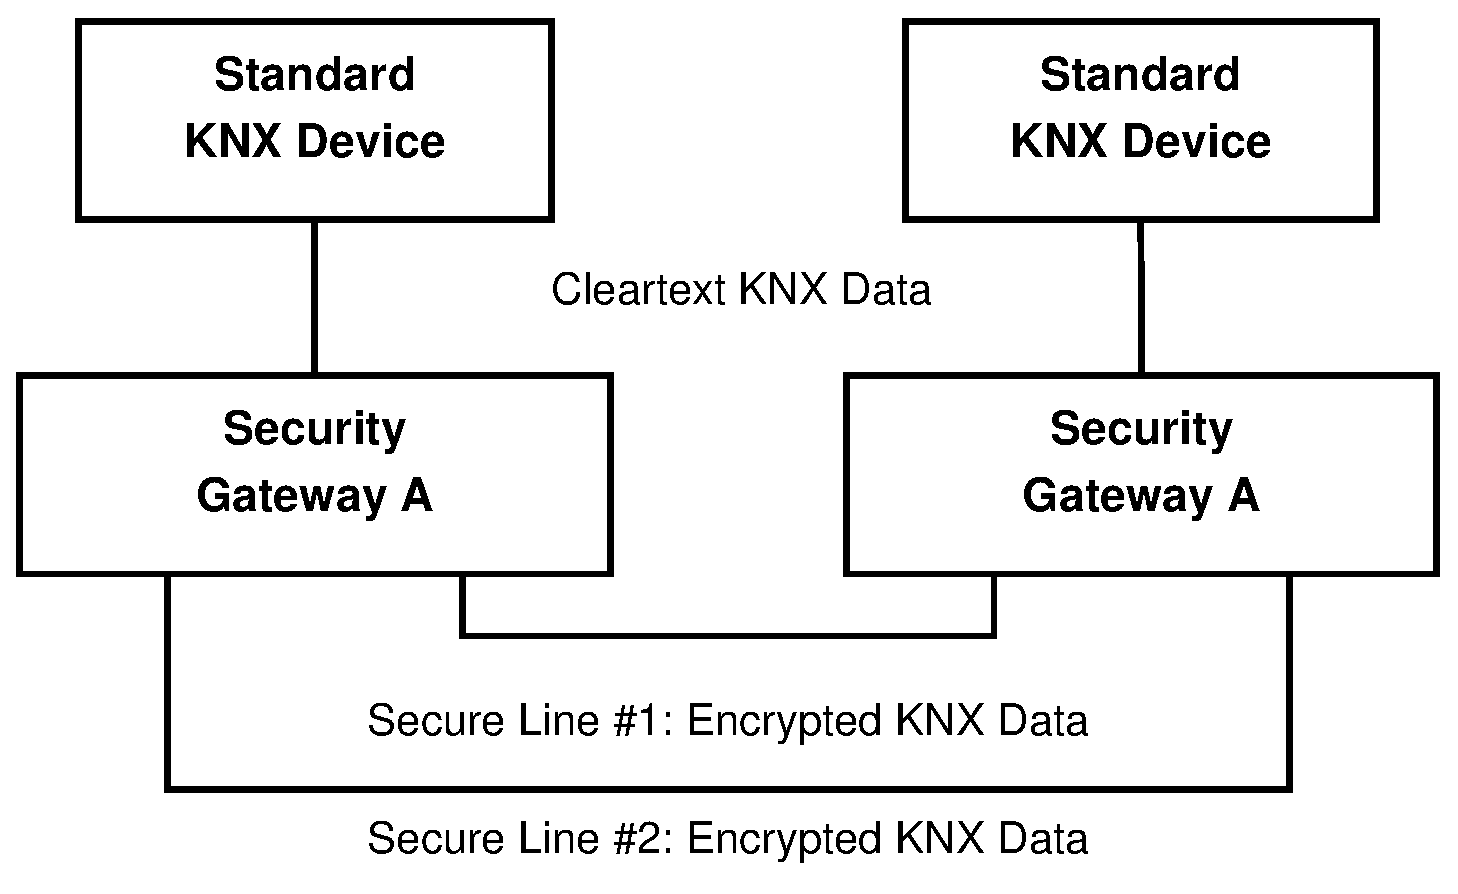
\includegraphics[width=1\textwidth]{figures/SecureArea.eps}
    \caption{Secure Area}
    \label{fig:secArea}
\end{figure}
\\
\\
A straightforward solution to this problem would be to wrap every datagram which enters the secured \gls{knx} network via a security gateway into a new, properly secured
broadcast datagram, and delivering this new package to the secured \gls{knx} network. Then, the package would be available to all other security gateways, which
will unwrap it and forward the resulting inner datagram to its unsecured \gls{knx} line. If the destination address (group or individual) of the actual payload
is assigned to a device connected
to the unsecured \gls{knx} network, the device holding this \gls{ia} or \gls{ga} will recognize it and the package will reach its destination. 
Otherwise it will simply be discarded.
\\
A serious constraint rising from this broadcast approach is that a single,
global network key must be used, because every security gateway must be able to decrypt and check every package which it receives on it's secured lines,
even if it does not serve as gateway to the wanted group address. 
The key of course can be renegotiated among the security gateways at every time, but this approach is considered
unsafe because an attacker can target \textit{any} of the security gateways constituting the secure network. An adversary breaking one single device gains
access to the network traffic of all devices. This could be achieved by physical access to any of the security gateways, for example by reading out the
memory of the device, and thus obtaining the globally used network key. This way, the network traffic can be decrypted by the adversary as long as no new
key is renegotiated. Another problem is that multi-party key negotiation is a costly task if a public-private key scheme
is to be used: as shown in figures \ref{fig:dh1} and \ref{fig:dh2}, a lot of messages have to be exchanged before actual an encryption can be done. 
\\
\\
To encounter this problems, different keys must be used, thus achieving pairwise end-to-end encryption between all devices. 
%This way it is also possible to achieve different security levels, depending on the function a 
%particular unsecured \gls{knx} device fulfills. It would be possible, for example, to distinguish between 'normal' gateways and 'hardened'
%gateways which are specially guarded against physical access, for example by applying physical intrusion detection. Thus,
%the risk of breaking the whole system is reduced, because breaking a device in one security level does not affect the security of the devices with other
%security levels.
%So, for breaking all $n$ security levels of a system, at least $n$ devices, all belonging to different levels must be broken.
%As a motivating example, imagine a setup which consists of window controls in an upper floor, and door controls in the
%base level. Obviously, the security constraints for the latter one would be higher. By using normal devices for window control, and hardened devices for
%door control, a security firewall can be deployed, thus containing the damage an adversary can do to the whole system.
Figure \ref{fig:firewall} shows the logical connections within an \gls{knx} network using end-to-end encryption. An 
attack of node $A$ can only compromise keys known to the device, thus effectively separating communication between the nodes $B$, $C$, and $D$ from
the attacker. 
\begin{figure}
  \centering
    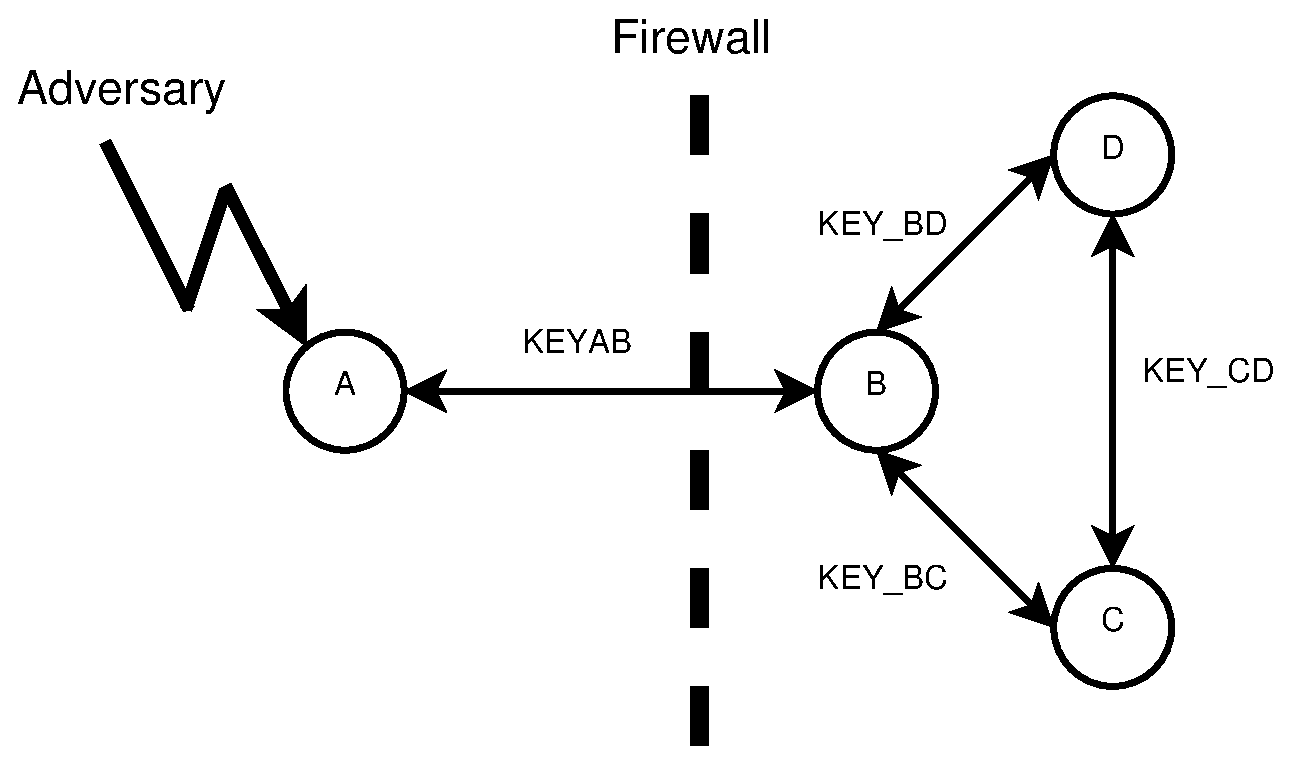
\includegraphics[width=0.8\textwidth]{figures/firewall2.eps}
% % Graphic for TeX using PGF
% Title: /home/hglanzer/ownCloud/Diplomarbeit/MasterThesisTemplate/figures/firewall.dia
% Creator: Dia v0.97.2
% CreationDate: Fri Dec  5 19:14:47 2014
% For: hglanzer
% \usepackage{tikz}
% The following commands are not supported in PSTricks at present
% We define them conditionally, so when they are implemented,
% this pgf file will use them.
\ifx\du\undefined
  \newlength{\du}
\fi
\setlength{\du}{15\unitlength}
\begin{tikzpicture}
\pgftransformxscale{1.000000}
\pgftransformyscale{-1.000000}
\definecolor{dialinecolor}{rgb}{0.000000, 0.000000, 0.000000}
\pgfsetstrokecolor{dialinecolor}
\definecolor{dialinecolor}{rgb}{1.000000, 1.000000, 1.000000}
\pgfsetfillcolor{dialinecolor}
\pgfsetlinewidth{0.100000\du}
\pgfsetdash{}{0pt}
\pgfsetdash{}{0pt}
\pgfsetbuttcap
\pgfsetmiterjoin
\pgfsetlinewidth{0.100000\du}
\pgfsetbuttcap
\pgfsetmiterjoin
\pgfsetdash{}{0pt}
\definecolor{dialinecolor}{rgb}{1.000000, 1.000000, 1.000000}
\pgfsetfillcolor{dialinecolor}
\pgfpathellipse{\pgfpoint{12.000000\du}{5.000000\du}}{\pgfpoint{1.000000\du}{0\du}}{\pgfpoint{0\du}{1.000000\du}}
\pgfusepath{fill}
\definecolor{dialinecolor}{rgb}{0.000000, 0.000000, 0.000000}
\pgfsetstrokecolor{dialinecolor}
\pgfpathellipse{\pgfpoint{12.000000\du}{5.000000\du}}{\pgfpoint{1.000000\du}{0\du}}{\pgfpoint{0\du}{1.000000\du}}
\pgfusepath{stroke}
\pgfsetbuttcap
\pgfsetmiterjoin
\pgfsetdash{}{0pt}
\definecolor{dialinecolor}{rgb}{0.000000, 0.000000, 0.000000}
\pgfsetstrokecolor{dialinecolor}
\pgfpathellipse{\pgfpoint{12.000000\du}{5.000000\du}}{\pgfpoint{1.000000\du}{0\du}}{\pgfpoint{0\du}{1.000000\du}}
\pgfusepath{stroke}
\pgfsetlinewidth{0.100000\du}
\pgfsetdash{}{0pt}
\pgfsetdash{}{0pt}
\pgfsetbuttcap
\pgfsetmiterjoin
\pgfsetlinewidth{0.100000\du}
\pgfsetbuttcap
\pgfsetmiterjoin
\pgfsetdash{}{0pt}
\definecolor{dialinecolor}{rgb}{1.000000, 1.000000, 1.000000}
\pgfsetfillcolor{dialinecolor}
\pgfpathellipse{\pgfpoint{18.000000\du}{1.000000\du}}{\pgfpoint{1.000000\du}{0\du}}{\pgfpoint{0\du}{1.000000\du}}
\pgfusepath{fill}
\definecolor{dialinecolor}{rgb}{0.000000, 0.000000, 0.000000}
\pgfsetstrokecolor{dialinecolor}
\pgfpathellipse{\pgfpoint{18.000000\du}{1.000000\du}}{\pgfpoint{1.000000\du}{0\du}}{\pgfpoint{0\du}{1.000000\du}}
\pgfusepath{stroke}
\pgfsetbuttcap
\pgfsetmiterjoin
\pgfsetdash{}{0pt}
\definecolor{dialinecolor}{rgb}{0.000000, 0.000000, 0.000000}
\pgfsetstrokecolor{dialinecolor}
\pgfpathellipse{\pgfpoint{18.000000\du}{1.000000\du}}{\pgfpoint{1.000000\du}{0\du}}{\pgfpoint{0\du}{1.000000\du}}
\pgfusepath{stroke}
\pgfsetlinewidth{0.100000\du}
\pgfsetdash{}{0pt}
\pgfsetdash{}{0pt}
\pgfsetbuttcap
\pgfsetmiterjoin
\pgfsetlinewidth{0.100000\du}
\pgfsetbuttcap
\pgfsetmiterjoin
\pgfsetdash{}{0pt}
\definecolor{dialinecolor}{rgb}{1.000000, 1.000000, 1.000000}
\pgfsetfillcolor{dialinecolor}
\pgfpathellipse{\pgfpoint{18.000000\du}{9.000000\du}}{\pgfpoint{1.000000\du}{0\du}}{\pgfpoint{0\du}{1.000000\du}}
\pgfusepath{fill}
\definecolor{dialinecolor}{rgb}{0.000000, 0.000000, 0.000000}
\pgfsetstrokecolor{dialinecolor}
\pgfpathellipse{\pgfpoint{18.000000\du}{9.000000\du}}{\pgfpoint{1.000000\du}{0\du}}{\pgfpoint{0\du}{1.000000\du}}
\pgfusepath{stroke}
\pgfsetbuttcap
\pgfsetmiterjoin
\pgfsetdash{}{0pt}
\definecolor{dialinecolor}{rgb}{0.000000, 0.000000, 0.000000}
\pgfsetstrokecolor{dialinecolor}
\pgfpathellipse{\pgfpoint{18.000000\du}{9.000000\du}}{\pgfpoint{1.000000\du}{0\du}}{\pgfpoint{0\du}{1.000000\du}}
\pgfusepath{stroke}
\pgfsetlinewidth{0.100000\du}
\pgfsetdash{}{0pt}
\pgfsetdash{}{0pt}
\pgfsetbuttcap
\pgfsetmiterjoin
\pgfsetlinewidth{0.100000\du}
\pgfsetbuttcap
\pgfsetmiterjoin
\pgfsetdash{}{0pt}
\definecolor{dialinecolor}{rgb}{1.000000, 1.000000, 1.000000}
\pgfsetfillcolor{dialinecolor}
\pgfpathellipse{\pgfpoint{24.000000\du}{5.000000\du}}{\pgfpoint{1.000000\du}{0\du}}{\pgfpoint{0\du}{1.000000\du}}
\pgfusepath{fill}
\definecolor{dialinecolor}{rgb}{0.000000, 0.000000, 0.000000}
\pgfsetstrokecolor{dialinecolor}
\pgfpathellipse{\pgfpoint{24.000000\du}{5.000000\du}}{\pgfpoint{1.000000\du}{0\du}}{\pgfpoint{0\du}{1.000000\du}}
\pgfusepath{stroke}
\pgfsetbuttcap
\pgfsetmiterjoin
\pgfsetdash{}{0pt}
\definecolor{dialinecolor}{rgb}{0.000000, 0.000000, 0.000000}
\pgfsetstrokecolor{dialinecolor}
\pgfpathellipse{\pgfpoint{24.000000\du}{5.000000\du}}{\pgfpoint{1.000000\du}{0\du}}{\pgfpoint{0\du}{1.000000\du}}
\pgfusepath{stroke}
\pgfsetlinewidth{0.100000\du}
\pgfsetdash{}{0pt}
\pgfsetdash{}{0pt}
\pgfsetbuttcap
{
\definecolor{dialinecolor}{rgb}{0.000000, 0.000000, 0.000000}
\pgfsetfillcolor{dialinecolor}
% was here!!!
\pgfsetarrowsstart{stealth}
\pgfsetarrowsend{stealth}
\definecolor{dialinecolor}{rgb}{0.000000, 0.000000, 0.000000}
\pgfsetstrokecolor{dialinecolor}
\draw (17.000000\du,1.000000\du)--(12.000000\du,4.000000\du);
}
\pgfsetlinewidth{0.100000\du}
\pgfsetdash{}{0pt}
\pgfsetdash{}{0pt}
\pgfsetbuttcap
{
\definecolor{dialinecolor}{rgb}{0.000000, 0.000000, 0.000000}
\pgfsetfillcolor{dialinecolor}
% was here!!!
\pgfsetarrowsstart{stealth}
\pgfsetarrowsend{stealth}
\definecolor{dialinecolor}{rgb}{0.000000, 0.000000, 0.000000}
\pgfsetstrokecolor{dialinecolor}
\draw (12.000000\du,6.000000\du)--(17.000000\du,9.000000\du);
}
\pgfsetlinewidth{0.100000\du}
\pgfsetdash{}{0pt}
\pgfsetdash{}{0pt}
\pgfsetbuttcap
{
\definecolor{dialinecolor}{rgb}{0.000000, 0.000000, 0.000000}
\pgfsetfillcolor{dialinecolor}
% was here!!!
\pgfsetarrowsstart{stealth}
\pgfsetarrowsend{stealth}
\definecolor{dialinecolor}{rgb}{0.000000, 0.000000, 0.000000}
\pgfsetstrokecolor{dialinecolor}
\draw (19.000000\du,9.000000\du)--(24.000000\du,6.000000\du);
}
\pgfsetlinewidth{0.100000\du}
\pgfsetdash{}{0pt}
\pgfsetdash{}{0pt}
\pgfsetbuttcap
{
\definecolor{dialinecolor}{rgb}{0.000000, 0.000000, 0.000000}
\pgfsetfillcolor{dialinecolor}
% was here!!!
\pgfsetarrowsstart{stealth}
\pgfsetarrowsend{stealth}
\definecolor{dialinecolor}{rgb}{0.000000, 0.000000, 0.000000}
\pgfsetstrokecolor{dialinecolor}
\draw (19.000000\du,1.000000\du)--(24.000000\du,4.000000\du);
}
\pgfsetlinewidth{0.100000\du}
\pgfsetdash{}{0pt}
\pgfsetdash{}{0pt}
\pgfsetbuttcap
{
\definecolor{dialinecolor}{rgb}{0.000000, 0.000000, 0.000000}
\pgfsetfillcolor{dialinecolor}
% was here!!!
\pgfsetarrowsstart{stealth}
\pgfsetarrowsend{stealth}
\definecolor{dialinecolor}{rgb}{0.000000, 0.000000, 0.000000}
\pgfsetstrokecolor{dialinecolor}
\draw (18.000000\du,2.000000\du)--(18.000000\du,8.000000\du);
}
\pgfsetlinewidth{0.300000\du}
\pgfsetdash{{1.000000\du}{1.000000\du}}{0\du}
\pgfsetdash{{1.000000\du}{1.000000\du}}{0\du}
\pgfsetbuttcap
{
\definecolor{dialinecolor}{rgb}{0.000000, 0.000000, 0.000000}
\pgfsetfillcolor{dialinecolor}
% was here!!!
\definecolor{dialinecolor}{rgb}{0.000000, 0.000000, 0.000000}
\pgfsetstrokecolor{dialinecolor}
\draw (15.707107\du,-1.388909\du)--(15.707107\du,11.611091\du);
}
% setfont left to latex
\definecolor{dialinecolor}{rgb}{0.000000, 0.000000, 0.000000}
\pgfsetstrokecolor{dialinecolor}
\node[anchor=west] at (18.292893\du,5.000000\du){$Key_{BC}$};
% setfont left to latex
\definecolor{dialinecolor}{rgb}{0.000000, 0.000000, 0.000000}
\pgfsetstrokecolor{dialinecolor}
\node[anchor=west] at (11.469670\du,4.893934\du){A};
% setfont left to latex
\definecolor{dialinecolor}{rgb}{0.000000, 0.000000, 0.000000}
\pgfsetstrokecolor{dialinecolor}
\node[anchor=west] at (17.505025\du,1.000000\du){B};
% setfont left to latex
\definecolor{dialinecolor}{rgb}{0.000000, 0.000000, 0.000000}
\pgfsetstrokecolor{dialinecolor}
\node[anchor=west] at (17.505025\du,9.000000\du){C};
% setfont left to latex
\definecolor{dialinecolor}{rgb}{0.000000, 0.000000, 0.000000}
\pgfsetstrokecolor{dialinecolor}
\node[anchor=west] at (23.505025\du,5.000000\du){D};
% setfont left to latex
\definecolor{dialinecolor}{rgb}{0.000000, 0.000000, 0.000000}
\pgfsetstrokecolor{dialinecolor}
\node[anchor=west] at (12.000000\du,2.000000\du){$Key_{AB}$};
% setfont left to latex
\definecolor{dialinecolor}{rgb}{0.000000, 0.000000, 0.000000}
\pgfsetstrokecolor{dialinecolor}
\node[anchor=west] at (12.000000\du,9.000000\du){$Key_{AC}$};
% setfont left to latex
\definecolor{dialinecolor}{rgb}{0.000000, 0.000000, 0.000000}
\pgfsetstrokecolor{dialinecolor}
\node[anchor=west] at (22.000000\du,2.000000\du){$Key_{BD}$};
% setfont left to latex
\definecolor{dialinecolor}{rgb}{0.000000, 0.000000, 0.000000}
\pgfsetstrokecolor{dialinecolor}
\node[anchor=west] at (22.000000\du,9.000000\du){$Key_{CD}$};
% setfont left to latex
\definecolor{dialinecolor}{rgb}{0.000000, 0.000000, 0.000000}
\pgfsetstrokecolor{dialinecolor}
\node[anchor=west] at (14.000000\du,9.000000\du){};
\pgfsetlinewidth{0.200000\du}
\pgfsetdash{}{0pt}
\pgfsetdash{}{0pt}
\pgfsetbuttcap
{
\definecolor{dialinecolor}{rgb}{0.000000, 0.000000, 0.000000}
\pgfsetfillcolor{dialinecolor}
% was here!!!
\definecolor{dialinecolor}{rgb}{0.000000, 0.000000, 0.000000}
\pgfsetstrokecolor{dialinecolor}
\draw (7.939094\du,0.782827\du)--(9.353307\du,3.611255\du);
}
\pgfsetlinewidth{0.200000\du}
\pgfsetdash{}{0pt}
\pgfsetdash{}{0pt}
\pgfsetbuttcap
{
\definecolor{dialinecolor}{rgb}{0.000000, 0.000000, 0.000000}
\pgfsetfillcolor{dialinecolor}
% was here!!!
\definecolor{dialinecolor}{rgb}{0.000000, 0.000000, 0.000000}
\pgfsetstrokecolor{dialinecolor}
\draw (9.303307\du,3.611255\du)--(9.975059\du,1.596000\du);
}
\pgfsetlinewidth{0.200000\du}
\pgfsetdash{}{0pt}
\pgfsetdash{}{0pt}
\pgfsetbuttcap
{
\definecolor{dialinecolor}{rgb}{0.000000, 0.000000, 0.000000}
\pgfsetfillcolor{dialinecolor}
% was here!!!
\pgfsetarrowsend{stealth}
\definecolor{dialinecolor}{rgb}{0.000000, 0.000000, 0.000000}
\pgfsetstrokecolor{dialinecolor}
\draw (9.975059\du,1.525290\du)--(11.353917\du,4.247651\du);
}
% setfont left to latex
\definecolor{dialinecolor}{rgb}{0.000000, 0.000000, 0.000000}
\pgfsetstrokecolor{dialinecolor}
\node[anchor=west] at (6.439525\du,0.358563\du){Adversary};
\end{tikzpicture}

 \caption{Firewall}
 \label{fig:firewall}
\end{figure}
As stated above, to be able to use different keys every security gateway has to know how to reach a given address so that the data can be encrypted
exclusively for the responsible gateway. The solution to this problem is to maintain some kind of routing table, mapping \glspl{ga} and \glspl{ia} of unsecured
\gls{knx} devices to \glspl{ia} of responsible security gateways	.
Such a routing table can be built statically at setup time, with the obvious disadvantage
that the exact topology of the to be applied network has to be known in advance, thus reducing the flexibility. Here, every security gateway holds a static 
table which consists of mappings between \glspl{ia} or \glspl{ga} of unsecured \gls{knx} devices and \glspl{ia} of security gateways at the border
between the secured and the unsecured \gls{knx} network, as well as all keys used for the particular security level the gateway belongs to.
This table would be generated once, after the topology of the network has been fixed, and must be equipped with the proper keys and can then
be copied to the security gateways constituting the secured \gls{knx} area. New security gateways can be deployed as long as they only introduce sending 
unsecured \gls{knx} devices, whose recipients are already mapped, known group addresses. A new group address, introduced by a newly installed device behind
an already existing security gateway, will not be reachable, simply because the routing information is not available. 
Another disadvantage is that the deployment of new
security gateways, connecting devices with new or already known \glspl{ga}, is impossible as the \gls{ia} of the new gateway - which of
course must be unique - is unknown to the existing setup, thus making the new unsecured \gls{knx} devices unreachable.
\\
To tackle this problem, another approach would be to build this mapping table dynamically. Therefore, every security gateway must periodically poll
on it's unsecured lines for \gls{knx} devices, thus populating a list of reachable \gls{knx} devices. Whenever a 
device wants to send data to a group address, it has to do a lookup first to obtain the \glspl{ia} of the responsible security gateways: the lookup
must contain the wanted group address, as well as the senders public key.
Every 
gateway which finds the wanted group address in its group list must reply with an according message to the requester, thus announcing that it is responsible
for delivering data to the wanted group address, and must also publish it's own public key, thus allowing pairwise end-to-end encryption.
This procedure requires no a priori knowledge of
the network topology, so security gateways can be added to the network as well as unsecured \gls{knx} devices behind new or existing gateways at any time. This
flexibility of course has to be purchased with increased complexity as well as additional traffic introduced into the network.
\\
\\
A middle course is chosen: the reachable group address list is generated whenever a new security gateway is added to the network,
 handling discovery of this group addresses as described
above. This allows to deploy new security gateways with connected unsecured devices, thus achieving a comprise between flexibility and complexity. 
\\
Sending data to a group address therefor follows the triad discovery request, discovery response and actual data transfer, shown in figure \ref{fig:prot1}. Broadcast
messages are depicted as solid end of the arrow, the rest denoting unicast messages.
\begin{figure}
  \centering
    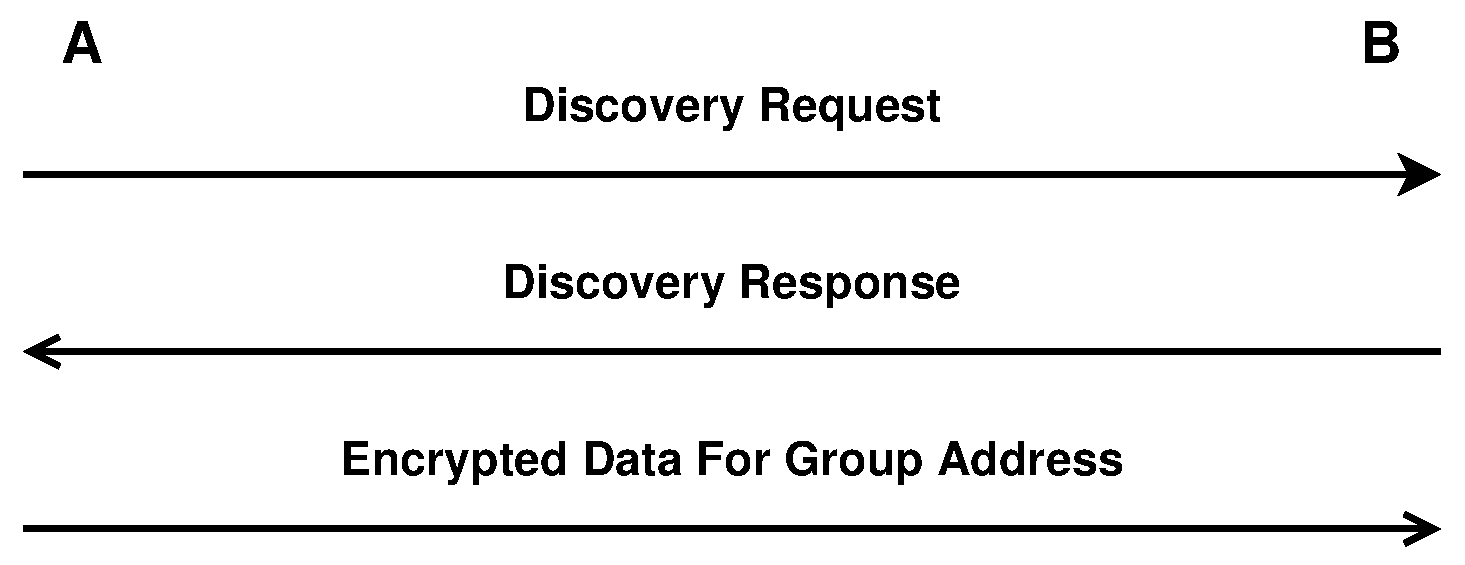
\includegraphics[width=0.8\textwidth]{figures/protokoll1.eps}
 \caption{Communication schema}
 \label{fig:prot1}
\end{figure}
To enable multiple devices to announce responsibility for a group address, the device wanting to transmit data to this group address must accept discovery responses
following it's request message for a short time window.
\\
\\
The discovery messages generated by security gateways should be encrypted too. Although these datagrams don't contain \gls{knx} data per se, they allow
a listening adversary to learn the topology of the network, knowledge which can be valuable for developing an attack strategy, as well as generating meta data.
For example, if an attacker learns that a particular security gateway is responsible for only one group address and further gets knowledge that this 
group address is responsible for switching a light (i.e. by visual observation), the attacker afterwards may be able to derive a personal profile just by seeing
packages for this group address, although the payload of the datagrams to the responsible security gateway are encrypted.
If the discovery messages are encrypted too the adversary doesn't know how many and what
group addresses are behind a specif gateway, and it will be harder to derive personal profiles or to gather knowledge of the network topology.
\\
Discovery request messages must be broadcast messages, readable by all security gateways. To limit the protocol overhead, a global network key is used here.
\\
\\
To provide authenticity, all datagrams passing the secured \gls{knx} network must contain a \gls{mac2} to prevent modification of them.
\\
Defense against replay attacks is achieved by counters.These must be strictly monotonically
increasing and must not overflow. The counters can be compared to an initialization vector that prevents the mapping of same cleartext messages to same ciphertext messages
under the same encryption key.
\\
Two different types of counters are used: one global counter $Ctr_{global}$, used for avoiding replay attacks against discovery messages. A second kind of counter
is used for the actual data transfer. Beside avoiding replay attacks, this counter is necessary to detect and delete duplicates, caused by the redundant network, 
see \ref{ctrAvail} for details.
\\
Usage of the global counter $Ctr_{global}$ raises another question, namely how a new device gets knowledge of the actual value of $Ctr_{global}$.
Therefor, a synchronization service must be defined, allowing a newly powered up device to synchronize with the rest of the network \ref{fig:syncProt}.
\begin{figure}
  \centering
    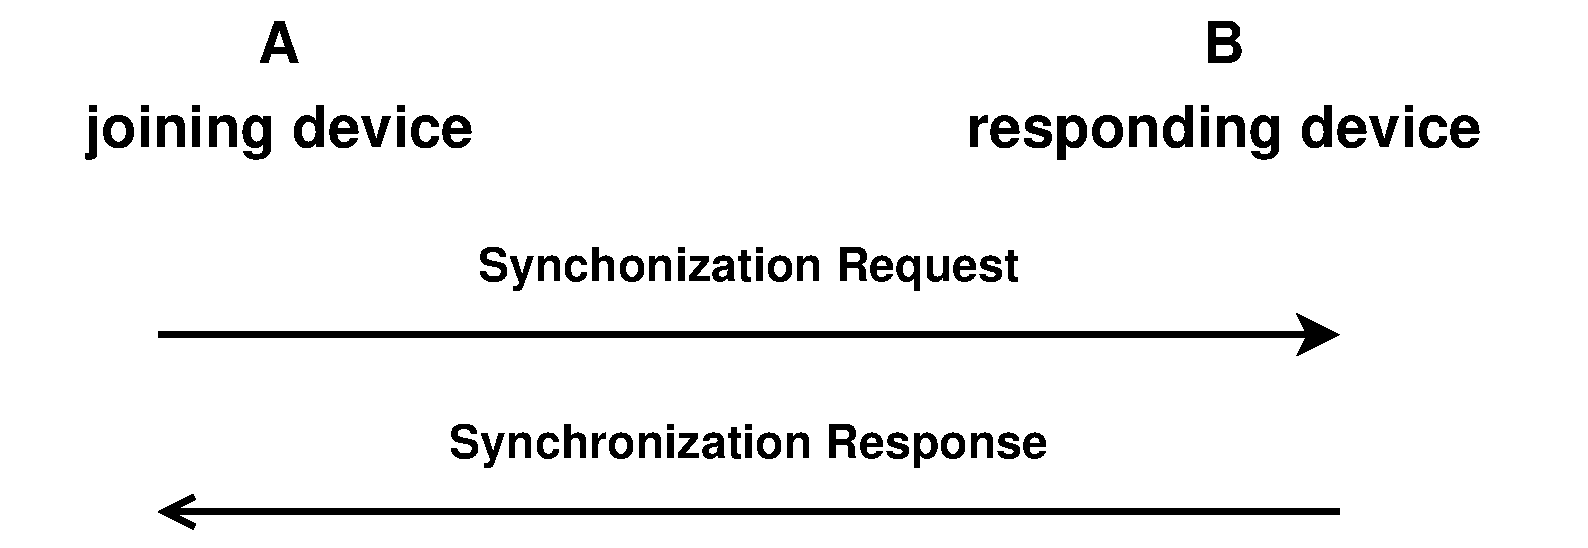
\includegraphics[width=0.8\textwidth]{figures/protSync.eps}
 \caption{Synchronization service}
 \label{fig:syncProt}
\end{figure}
Replay attacks are mitigated by including the actual time into \gls{mac2} calculation. Low temporal resolution relaxes time-synchronization issues between
different devices.

\subsubsection{Key Management}

While it would be possible to use a centralized concept, no trusted on-line party is used in this work. A centralized approach would need fall-back key servers
which inherit the task of generating and distributing keys and parameters in case of a master key server failure. Otherwise, the network would suffer from a
single point of failure in case no such fall-back mechanism is applied, an assumption that would clearly disqualify the design as highly available.
\\
The following keys are used:

\begin{itemize}
 \item A long-term key known to all security gateways is used. As already stated, this key must be copied to every device at setup time. 
This pre-shared key $k_{psk}$ is used for symmetric encryption and serves different purposes: first, it is used to authenticate synchronization messages.
Secondly, this key $k_{psk}$ is used to encrypt discovery requests and discovery responses.
 %\item $k_{global}$ is used to authenticate and encrypt locally generated and decrypt received discovery requests, as well as to authenticate and encrypt
 %locally generated discovery responses and decrypt received ones. These discovery service datagrams securely transport the third type of keys:
 \item Asymmetric keys are used for end-to-end encryption of the actual data packages between 2 security gateways. \gls{ecdh} serves as key negotiation algorithm.
 To protect against man-in-the-middle attacks, authenticity of the \gls{dh} parameters must be assured.
 \item This is the task of the third kind of keys: another pre-shared key is used to authenticate the \gls{dh} parameters.
\end{itemize}


\subsection{Redundancy Related Architectural Overview}\label{ctrAvail}
 
Whenever a \gls{knx} package is
generated by a device on an unsecured line (called client), the connected security gateway will read, duplicate and encapsulate it into another \gls{knx} frame 
and then send over booth lines. If booth lines are available, i.e. there is, for example, no shortcut, the security gateway responsible for forwarding the frame
will receive 2 different \gls{knx} frames encapsulating the same
payload, which itself is the \gls{knx} frame generated by the \gls{knx} client device in the first place. 
One message must be discarded to avoid duplicates. 
This is achieved with a monotonically increasing counter that also guards against replay attacks: whenever a package, generated by a client, enters the
network, a counter for outgoing packages is incremented, called $Ctr_{out}$, and is sent along the message. 
This counter must be unambiguously referenced by the origin cleartext message. 
The receiving side must maintain a counter for incoming packets, called $Ctr_{in}$, which will be updated by the received counter value
as soon as the first frame is received if the received value is higher than the saved one.
Subsequent delivery of the duplicate can be detected because the containing counter value equals the saved counter value.
\\
\\
To identify duplicate frames, basically various possibilities exist:
\\
Referencing booth $Ctr_{out}$ and $Ctr_{in}$ by the \gls{ga} of the origin cleartext message does only work if for every destination
 \gls{ga} in the network, at most one sending client device exists. Assuming client device $A$ and afterwards client device $B$ want to send the first message to
 the same destination \gls{ga}, the delivery of the message
 originating from device $A$ will trigger an update of the corresponding counter $Ctr_{in}$ at the responsible gateway, but device $B$ will use it's own counter
 for the outgoing message. Because device's $B$ outgoing counter is less than the gateway's actual incoming counter, both frames will be discarded by the gateway.
Therefor, this is no viable solution.
\\
\\
It shows that the easiest way to unambiguously identify duplicates is by referencing booth $Ctr_{out}$ and $Ctr_{in}$ by the \gls{ia} of the origin
cleartext message. This solution works despite potential network failures on one or booth secure lines, provided that each client device posses a unique
\gls{ia}. This is argued as follows:
\\
For simplicity, assume that 3 security gateways $A$, $B$ and $C$ are connected to each other by two distinct \gls{knx} lines, and each of them is connected
to an arbitrary number of client devices through their cleartext lines, each with an unique \gls{ia}.
Additionally, each client device is destination for an arbitrary number of \glspl{ga}.
If a security gateway receives a cleartext message, it will at first check the counter value $Ctr_{out}$ for the \gls{ia} and increment it. After that, the 
discovery phase takes place. This discovery request can be answered by zero, one or two other security gateways. If at least one reply is received, the package
is duplicated, encrypted, fitted into a unicast data frame together with $Ctr_{out}$ and sent on booth lines.
\\
Every gateway answering the discovery request will be sent 2 duplicate messages, one on each secure line. Now, there are 3 possibilities:
\begin{itemize}
 \item If booth secure lines are available, one data frame will be handled first and the contained counter will be saved as actual $Ctr_{in}$ for the \gls{ia}
 of the inner frame. When handling the second frame, the contained counter will be equal the saved counter, and thus the frame can be discarded.
 \item If only one secure line is available, no duplicate will arrive, but the receiving gateway(s) will nevertheless update the received counter value for the
 \gls{ia}
 \item If booth lines are unavailable, the responsible gateways cannot update the corresponding value for $Ctr_{in}$. Nevertheless, the sending side must update
 the outgoing counter $Ctr_{out}$. As soon as the responsible gateways are reachable again, new data frames will bear an even higher counter than saved on the
 receiving side, thus allowing data transfer to the \gls{ga} again.
\end{itemize}


%If booth lines are available, one message will be handled first and trigger an
%incrementation of the corresponding source address counter (i.e. the \gls{ga}).
%The duplicated message, which is handled after that, can safely be discarded because the corresponding counter value will be less than the saved value.

% Nevertheless which package from which secure line is forwarded to the unsecured line, each line must acknowledge
% every received package: this is done by generating a special acknowledge frame which is sent back to the sending gateway. The payload of this package must
% allow the sending gateway to unambiguously identify the acknowledged package, i.e. it must bear source and destination address of the package generated
% by the client, as well as the used counter value. As a consequence, these acknowledgement frames must be encrypted and authenticated as well.
% If no acknowledgement frame is received within time $t_{ACK}$, a retransmission is done on booth lines. This retransmission simply re-submits the same
% package with the same counter value again. Regarding the security this is no problem because a passive attacker can not learn anything from such a repeated
% package.


\subsection{Operational Constraints}

The introduction of encapsulating security gateways implicates that some timing constraints, defined by \gls{knx}, cannot be met:

\begin{itemize}
 \item Acknowledge frames, as defined in \gls{knx} and introduced in chapter \ref{ch:knx}, cannot be guaranteed to be delivered within the specified deadlines: whenever
 a new \gls{knx} datagram is generated by a client, at first the discovery phase has to occur. Only after that the to-acknowledged frame is sent. So there are
 multiple delays introduced, stalling the delivery: the first delay is caused by sending of the discovery package.
 After that, a second delay occurs because the security gateway must wait for the discovery response(s), possibly retransmitting the discovery request
 in case of a timeout. After receiving discovery responses, the third delay is caused by sending the actual, encapsulated
 client package to the responsible security gateway(s), which then must check the datagram, unpack it and forward it on it's unsecured line.
 Only after that, all addressed, unsecured clients would be able to acknowledge the received frames
 to their local security gateways,
 which must forwarded the acknowledgement frame to the origin security gateway, causing another delay. Finally, the acknowledgement frame must be forwarded to the sender of
 the origin data frame, causing another delay.
 These delays will always occur, and most of them cannot be restricted, thus destroying the tight timing constraints for acknowledgement frames, as defined
 by the \gls{knx} standard. This
 will most likely result in multiple retransmissions of the same \gls{knx} packages
 by the client because the client's timer will generate a timeout. The only way to solve this is to immediately acknowledge a client frame by the security
 gateway that it is connected to. On the receiving side, the client will generate an acknowledge
 frame, which must be discarded by it's security gateway.
 \item Similar arguments avoid the processing of Poll-Data Frames. Here, event more stringent timing constraints are to be met, see chapter \ref{ch:knx}. 
\end{itemize}

\section{Services}

Apart from the data service, handling the actual data transfer of the \gls{knx} payloads, 2 additional services are necessary, following the assumptions above.
These two services, handling synchronization and discovery, are defined as following and are summarized as management services. To distinguish the different
frame formats, a 8 bit \textit{secure header} field uniquely identifies every frame - see section \ref{secHdr} for details.

\begin{figure}
\begin{tikzpicture}[scale=0.2]
\tikzstyle{every node}+=[inner sep=2pt]
\tikzstyle{arrow}=[draw, -latex] 
\tikzset{
    pil/.style={
           ->,
           thick,
           shorten <=1pt,
           shorten >=1pt,}
}

\usetikzlibrary{automata,positioning}
\usetikzlibrary{positioning}

\node[state,initial]												at (45,35)			(init)		{Init}; 
\node[state, text width=2cm,align=center] 	at (60,35)		(sync)	{Send Sync Request};
\node[state, text width=1.5cm,align=center] 	at (45,20)	(fail)	{Failure}; 
\draw [black]	(45,20) circle (4);
\node[state, text width=1.5cm,align=center] 	at (85,25)		(res)	{Reset Counter};
\node[state, text width=1.8cm,align=center] 	at (60,15)		(chkFresh)	{Check Freshness};
\node[state, text width=1.8cm,align=center] 	at (85,10)		(rcv)	{Receive};
\node[state, text width=1.8cm,align=center] 	at (50,-15)		(chkMAC)	{Check MAC, Decrypt};
\node[state, text width=1.8cm,align=center] 	at (100,-15)		(discReq)	{Send Disc Request};
\node[state, text width=1.8cm,align=center] 	at (50,-40)		(sendResp)	{Send Response};
\node[state, text width=1.8cm,align=center] 	at (70,-25)		(chkDup)	{check Counter};
\node[state, text width=1.8cm,align=center] 	at (80,-40)		(fwd)	{Forward Message};
\node[state, text width=1.8cm,align=center] 	at (95,-40)		(sendDup)	{Send Duplicate};

\path[pil,->] (init)  edge[above] node[text width=1cm,align=center] {ok} (sync); 
\path[pil,->] (init)  edge[right] node[text width=0.5cm,align=center] {not ok} (fail); 
\path[pil,->] (sync)  edge[right,out=40,in=90] node[text width=1cm,align=center] {timeout} (sync); 
\path[pil,->] (sync)  edge[above] node[text width=2cm,align=center] {max retries} (res); 
\path[pil,->] (sync)  edge[right] node[text width=2cm,align=center] {valid response} (chkFresh); 
\path[pil,->] (chkFresh)  edge[right,out=120, in=200] node[text width=0.6cm,align=center] {not ok} (sync); 
\path[pil,->] (res)  edge[above] node[text width=2cm,align=center] {} (rcv); 
\path[pil,->] (chkFresh)  edge[above] node[text width=2cm,align=center] {OK} (rcv); 
\path[pil,->] (rcv)  edge[left] node[text width=1cm,align=center] {secure line} (chkMAC); 
\path[pil,->] (chkMAC)  edge[out=90,in=210] node[text width=2cm,align=center] {MAC invalid} (rcv); 
\path[pil,->] (rcv)  edge[right] node[text width=1cm,align=center] {clearext line} (discReq); 
\path[pil,->] (discReq)  edge[above,out=50,in=90] node[text width=1.2cm,align=center] {timeout} (discReq);
\path[pil,->] (discReq)  edge[] node[text width=2cm,align=center] {valid Response} (sendDup); 
\path[pil,->] (discReq)  edge[out=20,in=-20] node[text width=1.5cm,align=center] {max retries} (rcv); 
\path[pil,->] (chkMAC)  edge[left] node[text width=2cm,align=center] {mgmt message} (sendResp); 
\path[pil,->] (sendResp)  edge[left] node[text width=2.5cm,align=center] {} (rcv); 
\path[pil,->] (fwd)  edge[left] node[text width=1cm,align=center] {} (rcv); 
\path[pil,->] (chkMAC)  edge[above] node[text width=1.4cm,align=center] {KNX payload} (chkDup); 
\path[pil,->] (chkDup)  edge[] node[text width=1.5cm,align=center] {duplicate} (rcv); 
\path[pil,->] (chkDup)  edge[left] node[text width=1.5cm,align=center] {new message} (fwd); 
\path[pil,->] (sendDup)  edge[] node[text width=2cm,align=left] {} (rcv); 

\end{tikzpicture}
\label{fig:mainStateMachine}
\caption{State machine of the program logic}
\end{figure}

\subsection{Synchronization service}

As stated, a new gateway, joining the network, must get knowledge of the actual value of $Ctr_{global}$. This is achieved by sending a broadcast message on
ever secure line, 
serving as synchronization request. The frame  contains the device's local time in seconds. The header flags in the secure header are set accordingly, identifying
the frame as synchronization request \ref{fig:syncReqFormat}.
\begin{figure}
  \centering
    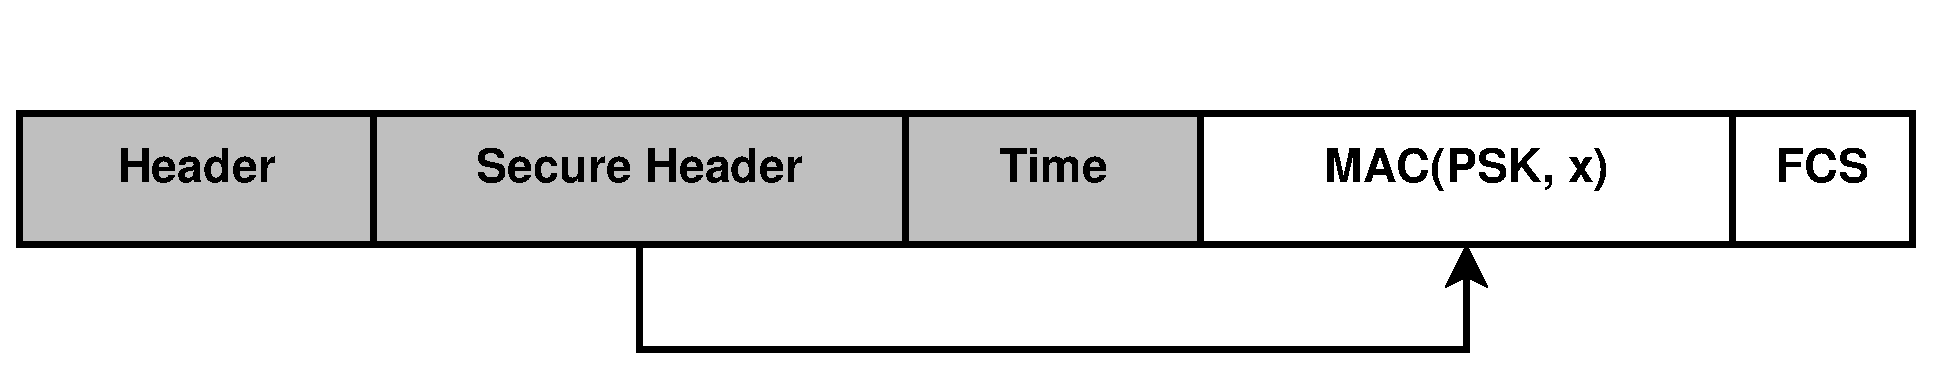
\includegraphics[width=1\textwidth]{figures/formatSyncReq.eps}
 \caption{Synchronization request frame layout}
 \label{fig:syncReqFormat}
\end{figure}
\\
\\
Every device receiving such a request checks the integrity of the message first by recalculating the \gls{mac2}. Afterwards, freshness is checked by comparing
the supplied time with it's local time. If the timing information equals the device's own local time, the device sends a unicast synchronization response
frame, containing it's local time and the actual counter value \ref{fig:syncResFormat}. The accuracy of the time comparison is deliberately reduced by defining
a window of allowed deviation. This allows a new device to join the network even it's local time and the local time of the answering device are not 
perfectly synchronized.
\begin{figure}
  \centering
    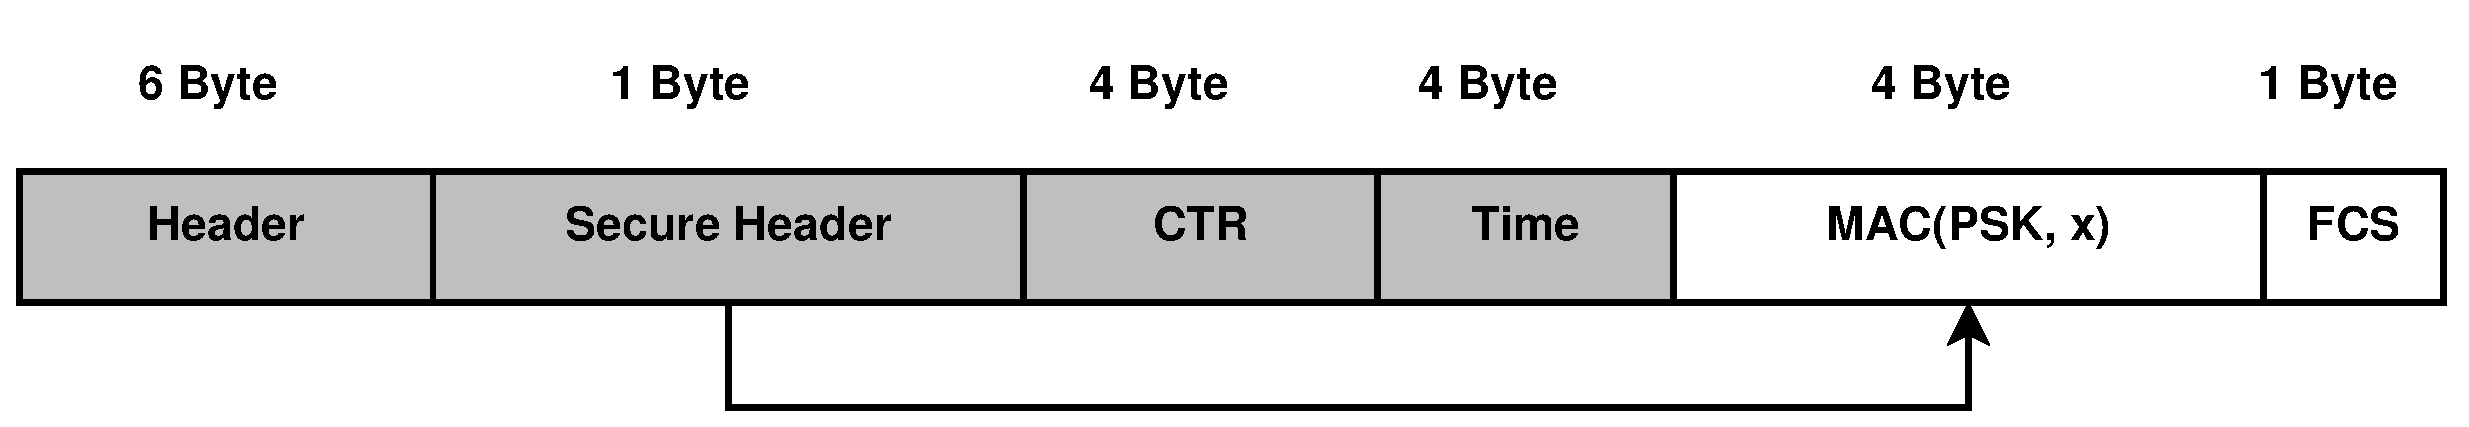
\includegraphics[width=1\textwidth]{figures/formatSyncRes.eps}
 \caption{Synchronization response frame layout}
 \label{fig:syncResFormat}
\end{figure}
If no synchronization response is received within 500ms, up to 2 retries are executed. After that, the device assumes that it is the first device in the
network and resets the global counter $Ctr_{global}$.
\\
\\
The \gls{mac2} is calculated over all frame fields except the trailing frame check fields and parts of the \textit{Header} field. 

\subsection{Discovery service}
Whenever a gateway receives a message on it's cleartext line, 2 distinct discovery broadcast messages are sent, one for each secured line. 
The frame format is shown in 
figure \ref{fig:discReqFormat}. \textit{DH-A} is the newly chosen \gls{ecdh} - parameter of the requesting device.
The \gls{psk} encrypted field contains the group address, CTR contains the incremented global counter $Ctr_{global}$.
\begin{figure}
  \centering
    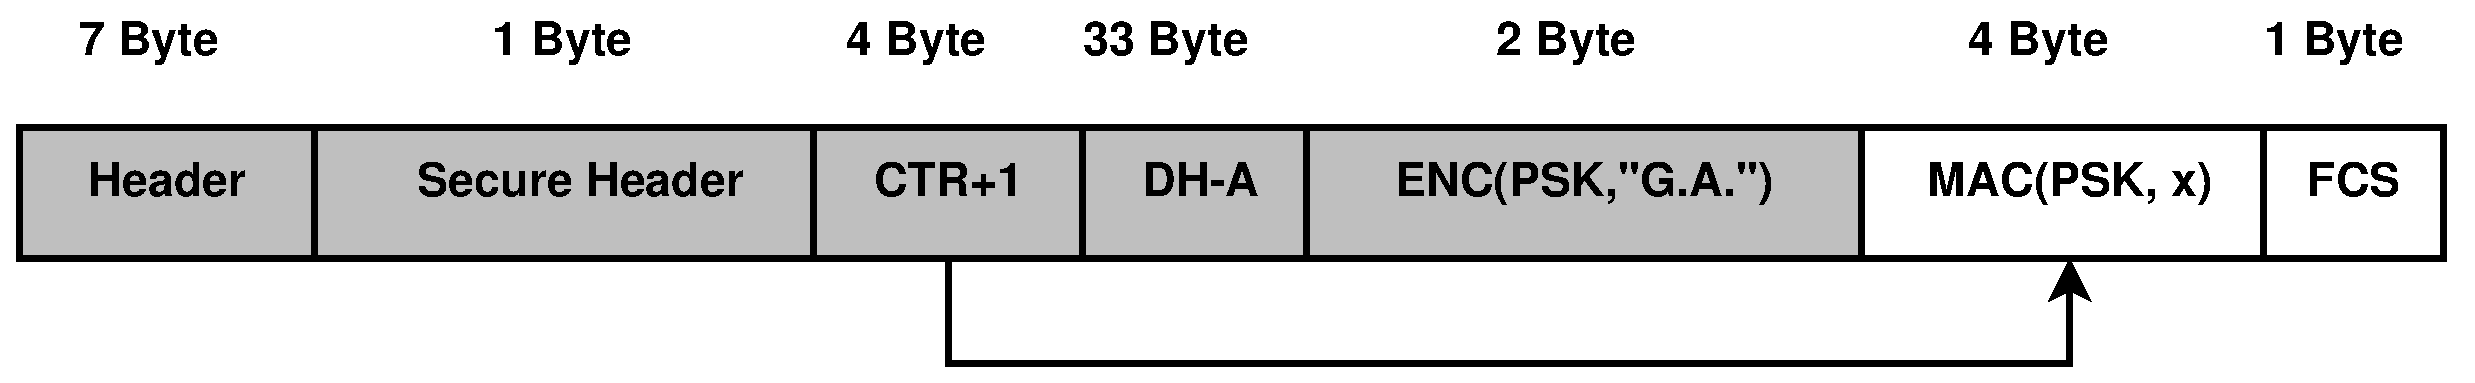
\includegraphics[width=1\textwidth]{figures/formatDiscReq.eps}
 \caption{Discovery request frame layout}
 \label{fig:discReqFormat}
\end{figure}
Every device in the network first checks the authenticity of the received frame by recalculating the \gls{mac2}. If the value differs the received one, the frame
is discarded. Otherwise, the requested group address is obtained by decrypting the corresponding field, and the device 
Every device recognizing the group address prepares a unicast response frame as shown in figure \ref{fig:discResFormat}, 
with \textit{DH-B} it's own newly chosen \gls{ecdh} parameter and the incremented global counter in the \textit{CTR} field. The wanted group address is also
sent, allowing the requester to identify the response message.
\begin{figure}
  \centering
    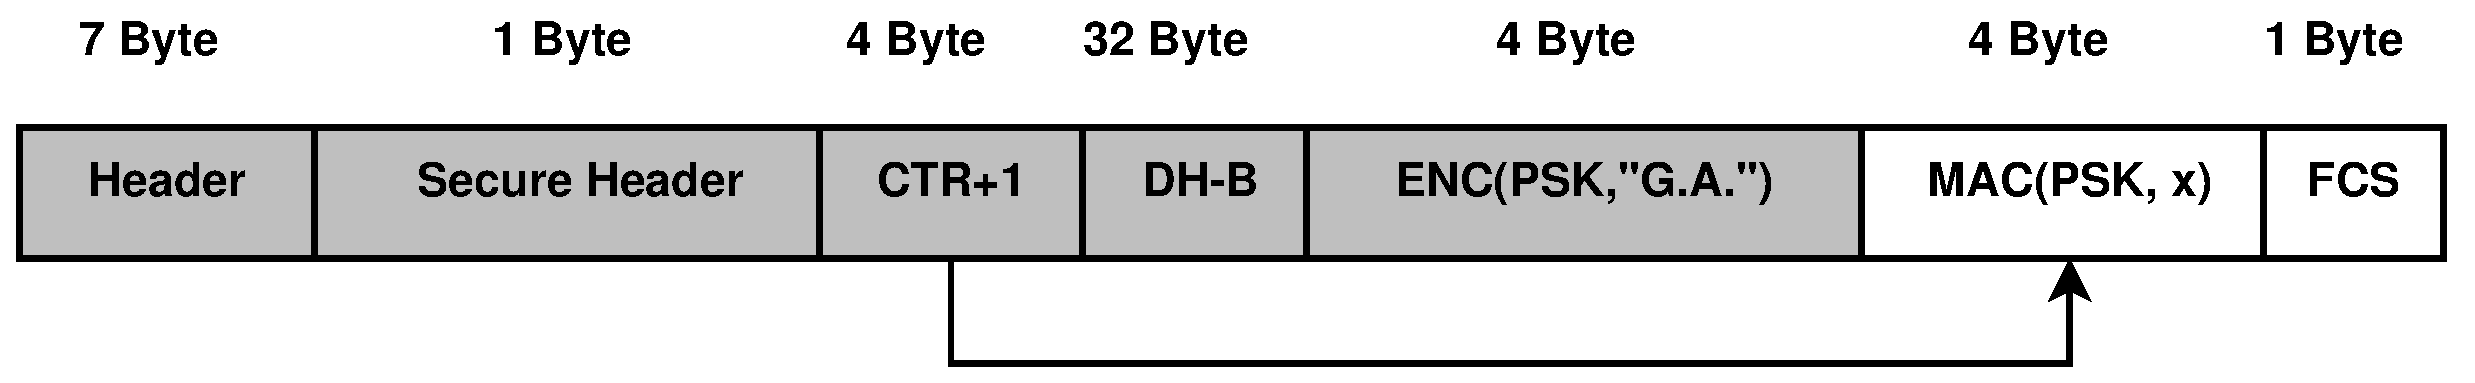
\includegraphics[width=1\textwidth]{figures/formatDiscResp.eps}
 \caption{Discovery response frame layout}
 \label{fig:discResFormat}
\end{figure}
\\
Integrity of the discovery messages is achieved by generating a \gls{mac2} over all frame fields except the frame check field and parts of the \textit{header}
field.
\\
The main logic from the discovery request receiver's point of view is shown in the state machine in \ref{fig:discRecv}

\begin{figure}
\centering
\begin{tikzpicture}[scale=0.2]
\tikzstyle{every node}+=[inner sep=4pt]
\tikzstyle{arrow}=[draw, -latex] 
\tikzset{
    pil/.style={
           ->,
           thick,
           shorten <=1pt,
           shorten >=1pt,}
}

\usetikzlibrary{automata,positioning}
\usetikzlibrary{positioning}

\node[state,initial]												at (15,0)			(rcv)		{Receive}; 
\node[state,text width=1.5cm,align=center]		at (0,-15)		(checkMAC) {Check MAC};
\node[state,text width=1.5cm,align=center]		at (-15,-30)		(discard) {Discard};
\node[state,text width=1.5cm,align=center]		at (15,-30)		(checkCtr) {Check Counter};
\node[state,text width=1.5cm,align=center]		at (0,-45)		(decrypt) {Decrypt};
\node[state,text width=1.5cm,align=center]		at (25,-45)		(sendReply) {Send Reply};

\path[pil,->] (rcv)  edge[] node[text width=1.5cm,align=center] {} (checkMAC); 
\path[pil,->] (discard)  edge[out=90,in=200] node[text width=1.5cm,align=center] {} (rcv); 
\path[pil,->] (checkMAC)  edge[] node[text width=1.5cm,align=left] {MAC invalid} (discard); 
\path[pil,->] (checkMAC)  edge[] node[text width=1.5cm,align=left] {MAC valid} (checkCtr); 
\path[pil,->] (checkCtr)  edge[] node[text width=1.5cm,align=center] {$\le Ctr_{global}$} (discard); 

\path[pil,->] (checkCtr)  edge[] node[text width=1.5cm,align=center] {$> Ctr_{global}$} (decrypt); 
\path[pil,->] (decrypt)  edge[] node[text width=1.5cm,align=center] {GA unknown} (discard); 
\path[pil,->] (decrypt)  edge[] node[text width=1.5cm,align=center] {GA known} (sendReply); 
\path[pil,->] (sendReply)  edge[out=90,in=300] node[text width=1cm,align=right] {} (rcv); 

\end{tikzpicture}
\caption{State machine for processing discovery requests}
\label{fig:discRecv}
\end{figure}

\subsection{Data service}
After receiving one or more discovery responses on one or booth secure line, the device which wants to send the \gls{knx} payload (called requester) now knows the
\glspl{ia} which are responsible for delivering messages to the wanted \gls{ga}. The requester can also derive a shared secret based on \gls{ecdh},
which is used to encrypt the origin \gls{knx} frame and inserted into the frame after the counter value. This counter $CTR-Ind$ is an individual counter, maintained
by the gateway forwarding the \gls{knx} frame received over the cleartext line - see \ref{ctrInd} for details.
\\
Authenticity is guaranteed by calculating a \gls{mac2} over all frame fields except the frame check field.
\\
\\
Figure \ref{fig:dataFormat} shows the layout of such a data frame.

\begin{figure}
  \centering
    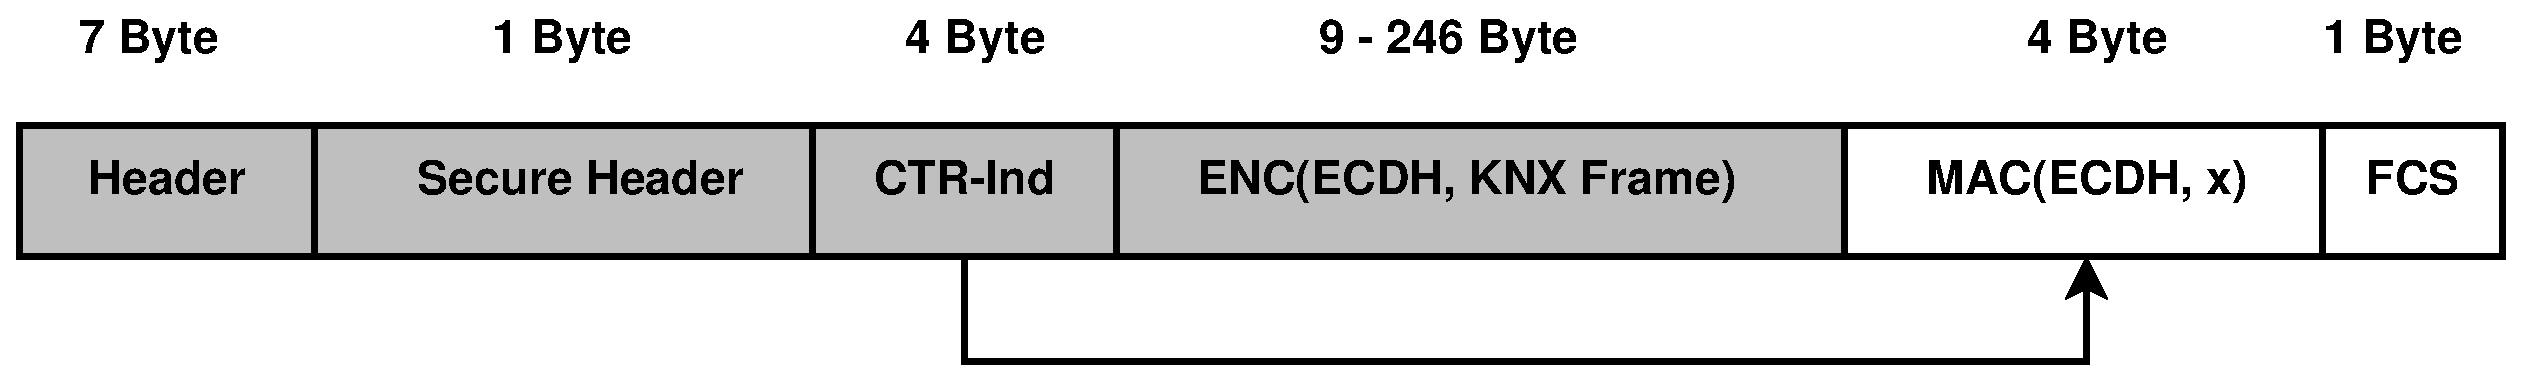
\includegraphics[width=1\textwidth]{figures/formatData.eps}
 \caption{Data  frame layout}
 \label{fig:dataFormat}
\end{figure}

\subsection{Data Structures}

The used data structures, referenced above, are introduced in more detail below.

\subsubsection{Secure header}\label{secHdr}
Every frame sent by a security gateway contains a 8 bit header, uniquely determining the type of the frame. Implicitly, this information also determines
the exact type of authentication, encryption or authenticated encryption mode used.

\begin{center}
\begin{tabular}{ c | c | c | c}
 \label{table:secHeader}
   bytevalue & frame type & encryption & authentication \\ \hline
   0000 0000 & invalid & x & x \\
   0000 0001 & invalid & x & x \\
   0000 0010 & synchronization request & no & yes \\
   0000 0011 & synchronization response & no & yes \\
   0000 0100 & discovery request & yes & yes \\
   0000 0101 & discovery response & yes & yes \\
   0000 1000 & data service & yes & yes \\
   0000 1001 & reserved & x & x \\
   ...  & ...  & ... & ... \\
   1111 1111 & reserved & x & x \\
\end{tabular}
\end{center}
Values 0x09 - 0xFF are not used - frames containing such values should be discarded.

\subsubsection{Global counter}\label{ctrInd}
The global counter $Ctr_{global}$ is a 4 byte integer, allowing $2^{32} \approx 4,3$ billion discovery request or response messages to be sent before overflowing,
an amount assumed sufficiently high, argued as follows:
each discovery messages consists of a frame containing 53 byte, sent with 9600 \gls{bps}, resulting in about 44 milliseconds transfer duration. Therefor,
the absolute lower bound of the duration after that $Ctr_{global}$ overflows, assumed the \gls{knx} network is occupied by discovery messages only,
is about 2 years, a very conservative estimate.

\subsubsection{Individual counter}\label{ctrInd}

Every individual counter is a 4 byte integer, responsible for duplicate detection. Two distinct types of individual counters are used: $Ctr_{out}$, referenced
by an \gls{ia}, and $Ctr_{in}$, also referenced by an \gls{ia}.
The main logic is shown in figure \ref{fig:dupSM}.
\\
Whenever a new \gls{knx} frame is received on the cleartext line and the gateway knows which gateway(s) are responsible for the
contained \gls{ga}, the sending gateway determines the outgoing counter value $Ctr_{out}[\gls{ia}]$. If an outgoing counter value for
this \gls{ia} exists 
this means that the device already sent at least one data frame to a \gls{ga}, otherwise this is the first frame. In both cases,
the counter value $Ctr_{out}[\gls{ia}]$ is incremented, saved and used as value for $Ctr_{ind}$. After that, the cleartext frame is
encrypted and inserted into a new unicast data frame, one for each secure line.
\\
\\
Upon reception (the green transition in \ref{fig:dupSM}), at first the validity of the \gls{mac2} is checked - if valid, the receiver checks it's incoming
individual counter value, referenced by the \gls{ia} of the inner frame. If the received counter value $Ctr_{ind}$ is smaller than $Ctr_{in}[\gls{ia}]$,
 $Ctr_{ind}$ is saved as $(Ctr_{in}[\gls{ia}]$ and the inner frame is forwarded. The second frame, which will be handled eventually 
afterwards will bear the counter value $Ctr_{ind} = Ctr_{in}[\gls{ia}]$ and will be discarded, thus eliminating the duplicate.

\begin{figure}
 \centering
\begin{tikzpicture}[scale=0.2]
\tikzstyle{every node}+=[inner sep=2pt]
\tikzstyle{arrow}=[draw, -latex] 
\tikzset{
    pil/.style={
           ->,
           thick,
           shorten <=1pt,
           shorten >=1pt,}
}

\usetikzlibrary{automata,positioning}
\usetikzlibrary{positioning}

\node[state,initial,text width=1cm,align=center]					at (0,-10)			(rcv)		{ rcv}; 
%\node[state,text width=2cm,align=center]					at (0,-15)			(chkCtr)		{Check Counter}; 
\node[state,text width=2.2cm,align=center]					at (-15,-30)			(ctrNew)		{$Ctr_{out}[IA] = 1$}; 
\node[state,text width=2.2cm,align=center]					at (15,-30)			(ctrKnown)	{ inc $Ctr_{out}[IA]$}; 
\node[state,text width=2.0cm,align=center]					at (0,-40)			(dup)		{duplicate, encrypt, send}; 
\node[state,text width=1.5cm,align=center]					at (-15,-55)			(rcv1)		{check MAC, decrypt}; 
\node[state,text width=1.5cm,align=center]					at (15,-55)			(rcv2)		{check MAC, decrypt}; 
\node[state,text width=1.4cm,align=center]					at (0,-70)			(discard)		{Discard}; 
\node[state,text width=1.5cm,align=center]					at (0,-90)			(chk)		{Check Counter}; 
\node[state,text width=1.4cm,align=center]					at (25,-90)			(fwd)		{Forward Frame}; 


\path[pil,->] (rcv)  edge[] node[text width=2cm,align=left] {$Ctr_{out}[IA]$ unknown} (ctrNew); 
\path[pil,->] (rcv)  edge[] node[text width=2cm,align=right] {$Ctr_{out}[IA]$ known} (ctrKnown); 
\path[pil,->] (ctrNew)  edge[] node[text width=1cm,align=right] {} (dup); 
\path[pil,->] (ctrKnown)  edge[] node[text width=3cm,align=right] {} (dup); 
\path[pil,->,color=green] (dup)  edge[out=200,in=90] node[text width=1cm,align=right] {} (rcv1); 
\path[pil,->,color=green] (dup)  edge[out=-20,in=90] node[text width=1cm,align=right] {} (rcv2); 
\path[pil,->] (rcv1)  edge[] node[text width=1.5cm] {MAC invalid} (discard); 
\path[pil,->] (rcv2)  edge[]   node[text width=1.5cm] {MAC invalid} (discard); 
\path[pil,->] (rcv1)  edge[out=270,in=135]   node[text width=1cm] {MAC valid} (chk); 
\path[pil,->] (rcv2)  edge[out=270,in=45]   node[text width=1cm] {MAC valid} (chk); 
\path[pil,->] (chk)  edge[]   node[text width=1cm] {$Ctr_{ind} \le Ctr_{in}[IA]$} (discard); 
\path[pil,->] (chk)  edge[]   node[text width=1cm] {$Ctr_{ind} > Ctr_{in}[IA]$} (fwd); 
% in / out dimension problem...
%\path[pil,->] (fwd)  edge[]   node[] {} (rcv); 

\end{tikzpicture}
\caption{State machine of the duplicate detection logic}
\label{fig:dupSM}
\end{figure}


%%%%%%%%%%%%%%%%%%%%%%%%%%%%%%%%%%%%%%%%%
%%% BACKMATTER %%%%%%%%%%%%%%%%%%%%%%%%%%
%%%%%%%%%%%%%%%%%%%%%%%%%%%%%%%%%%%%%%%%%

\appendix

%%%%%%%%%%%%%%%%%%%%%%%%%%%%%%%%%%%%%%%%%
\nocite{*}	% generate complete bibliography without corresponding \cites{}
\printbibliography

%%%%%%%%%%%%%%%%%%%%%%%%%%%%%%%%%%%%%%%%%

\printglossary

%%%%%%%%%%%%%%%%%%%%%%%%%%%%%%%%%%%%%%%%%
\chapter{Configuration Files}

\begin{lstlisting}[style=BashInputStyle,caption={Raspbian configuration for static ip address},label=lst:staticIP]
# device: eth0
  auto  eth0
  iface eth0 inet static
  address   192.168.0.2
  broadcast 192.168.0.255
  netmask   255.255.255.0
  gateway   192.168.0.1
\end{lstlisting}

\begin{lstlisting}[style=BashInputStyle,caption={Raspbian configuration for dynamic ip address},label=lst:dynamicIP]
# device: eth0
  iface eth0 inet dhcp
\end{lstlisting}

%\end{appendices}

\end{document}
